\chapter{Service work}
\clearpage

\section{HCAL logical map}
HCAL Logical map has been described in detail in the HCAL section in chapter 3. The HCAL map validation plots are listed here in different period and various sub-detectors. The FrontEnd electronics variables are the based coordinates that used in the validation plots. The validation plots are separated into 2 categories: BackEnd variables in FrontEnd coordinates and Geometry variables in FrontEnd coordinates. A complete FrontEnd coordinates set has 4 variables, RBX (readout box), RM (readout module), RM fibers and fiber channel for HB, HE and HO. HF is special since it does have RM (readout module). HF FrontEnd can be described by RBX, QIE10 slot, QIE10 fiber and fiber channel. BackEnd and Geometry variables will be described separately in the following sections.
\clearpage

\subsection{Remapped phase 1 HB in 2018}
The 2018 HB is still in HPD+QIE8 FrontEnd+uTCA BackEnd stage. We are in this hardware setting since 2016. However, HE will be upgraded to SiPM+QIE11 FrontEnd+uTCA BackEnd with more readout channels. Then the patch panels need to be reorganized since HB and HE share the same BackEnd electronics. The remapped 2018 HB is followed by the design from Richard Kellogg, coordinated with Jeremy Mans on the requirement of trigger sum algorithm in BackEnd firmware. 

The validation plots of remapped HB in 2018 are showed from Fig~\ref{fig:lmapHBPEtaFEC} to Fig~\ref{fig:lmapHBMuHTRFIFEC}. There are 2592 readout channels in total for remapped HB (same as 2016 HB, before remap). In order to satisfy the trigger latency requirement, the frontend channel permutation is applied in this map. HB BackEnd electronics are still in uTCA, 12 uHTR in one crate, 24 out going fibers per uHTR card, with 3 channels per fiber. 
\clearpage

\begin{figure}[htb]
 \begin{center}
  \begin{tabular}{cc}
   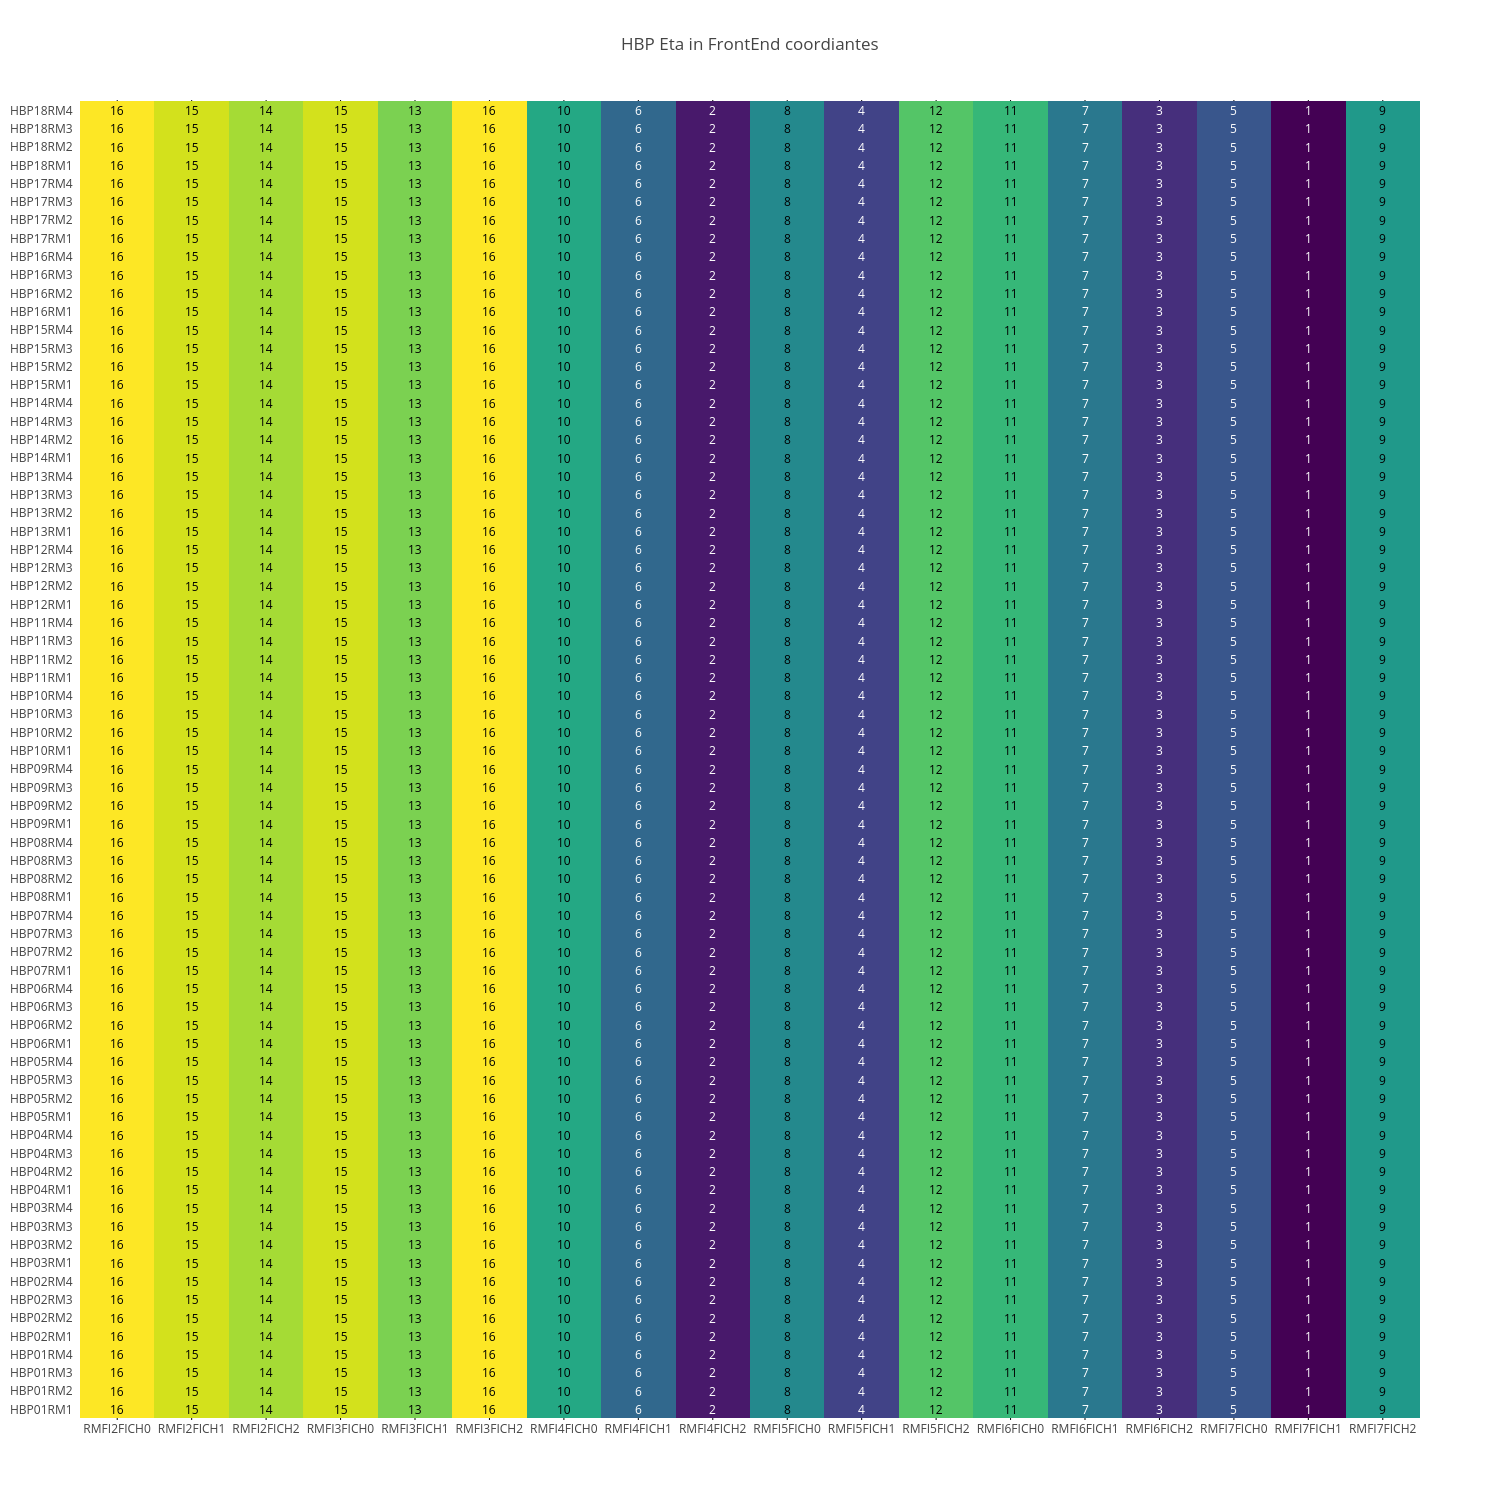
\includegraphics[angle=0,width=0.95\textwidth]{figures/appendix/HBP_Eta_in_FrontEnd.png}
  \end{tabular}
	\caption{HCAL (phase 1 HB, plus side) detector $\eta$ distribution in the frontend electronic coordinates.}
  \label{fig:lmapHBPEtaFEC}
 \end{center}
\end{figure}
\clearpage

\begin{figure}[htb]
 \begin{center}
  \begin{tabular}{cc}
   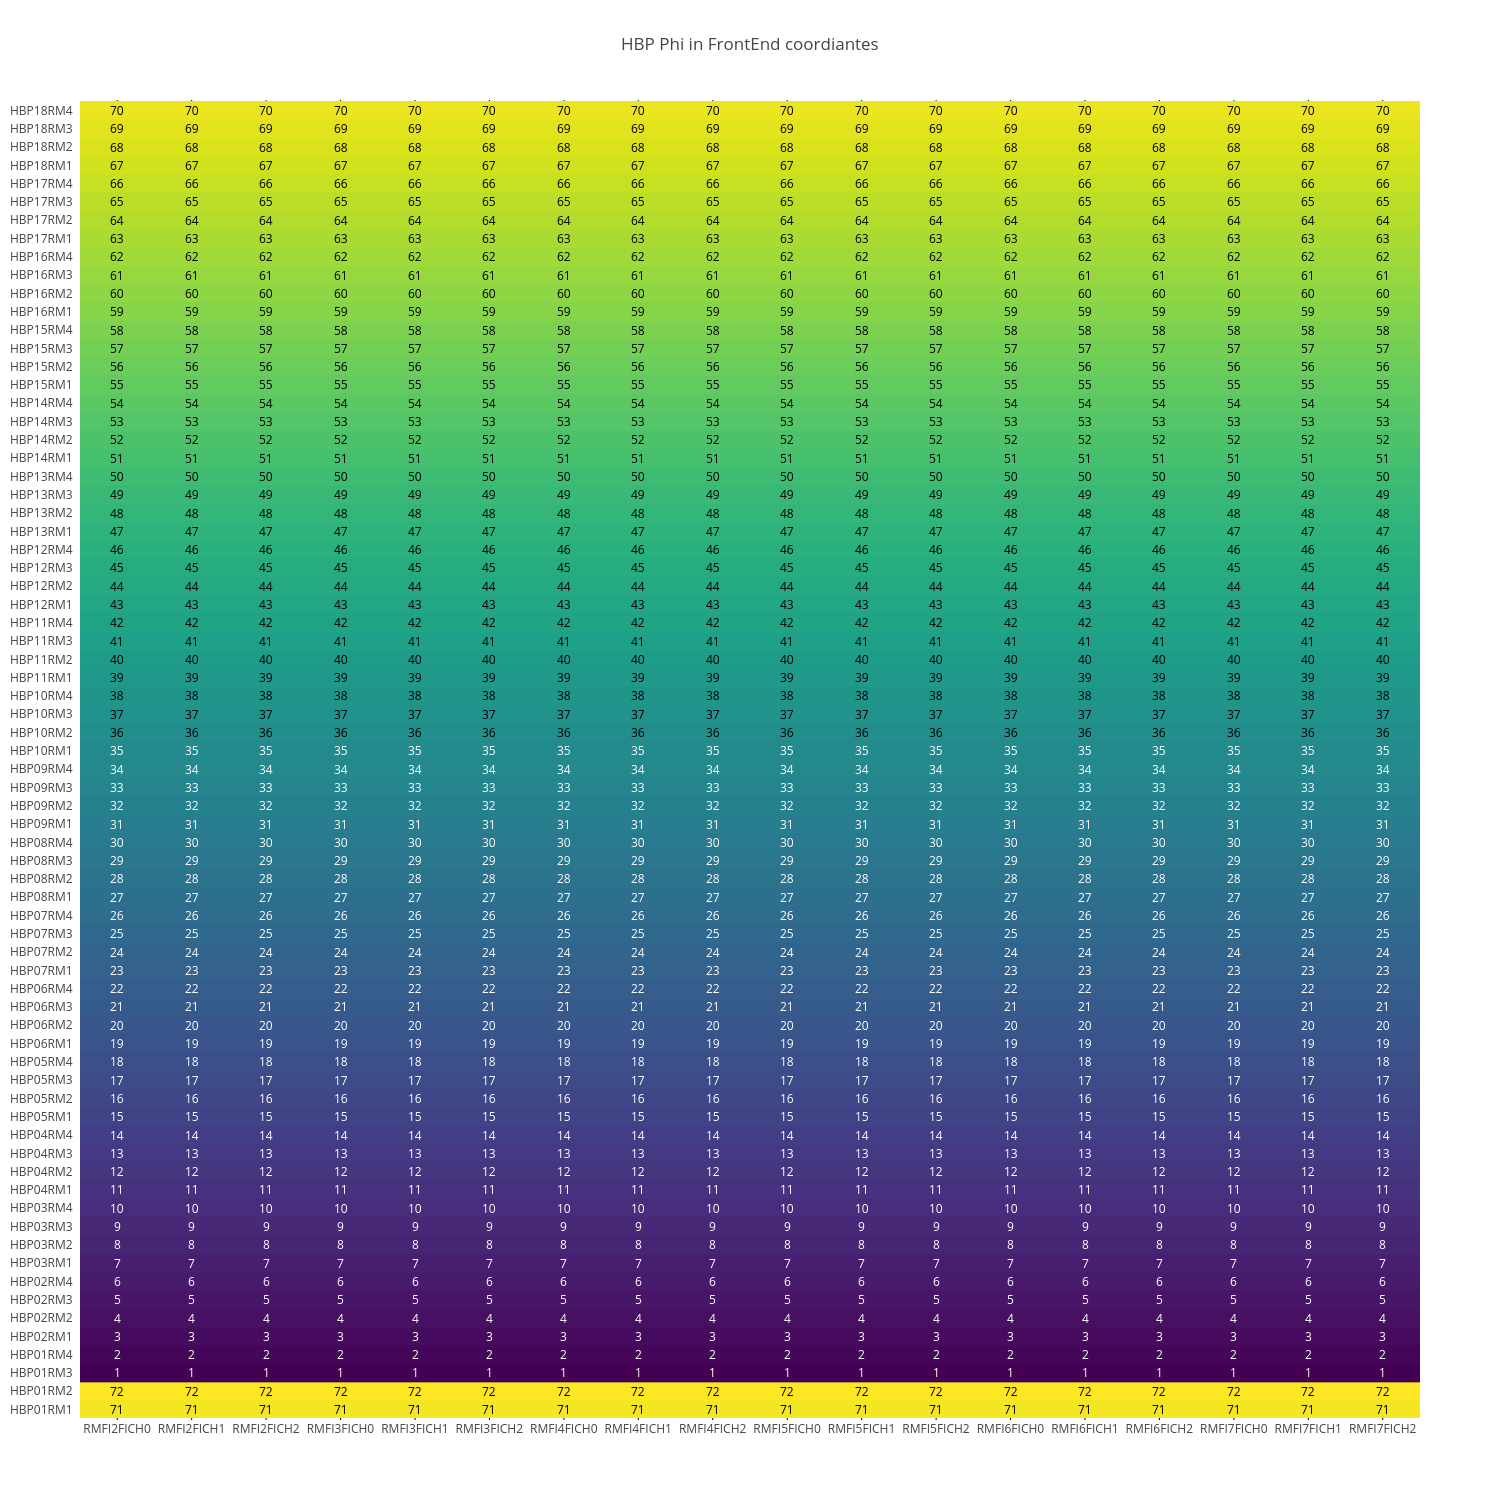
\includegraphics[angle=0,width=0.95\textwidth]{figures/appendix/HBP_Phi_in_FrontEnd.png}
  \end{tabular}
	\caption{HCAL (phase 1 HB, plus side) detector $\phi$ distribution in the frontend electronic coordinates.}
  \label{fig:lmapHBPPhiFEC}
 \end{center}
\end{figure}
\clearpage

\begin{figure}[htb]
 \begin{center}
  \begin{tabular}{cc}
   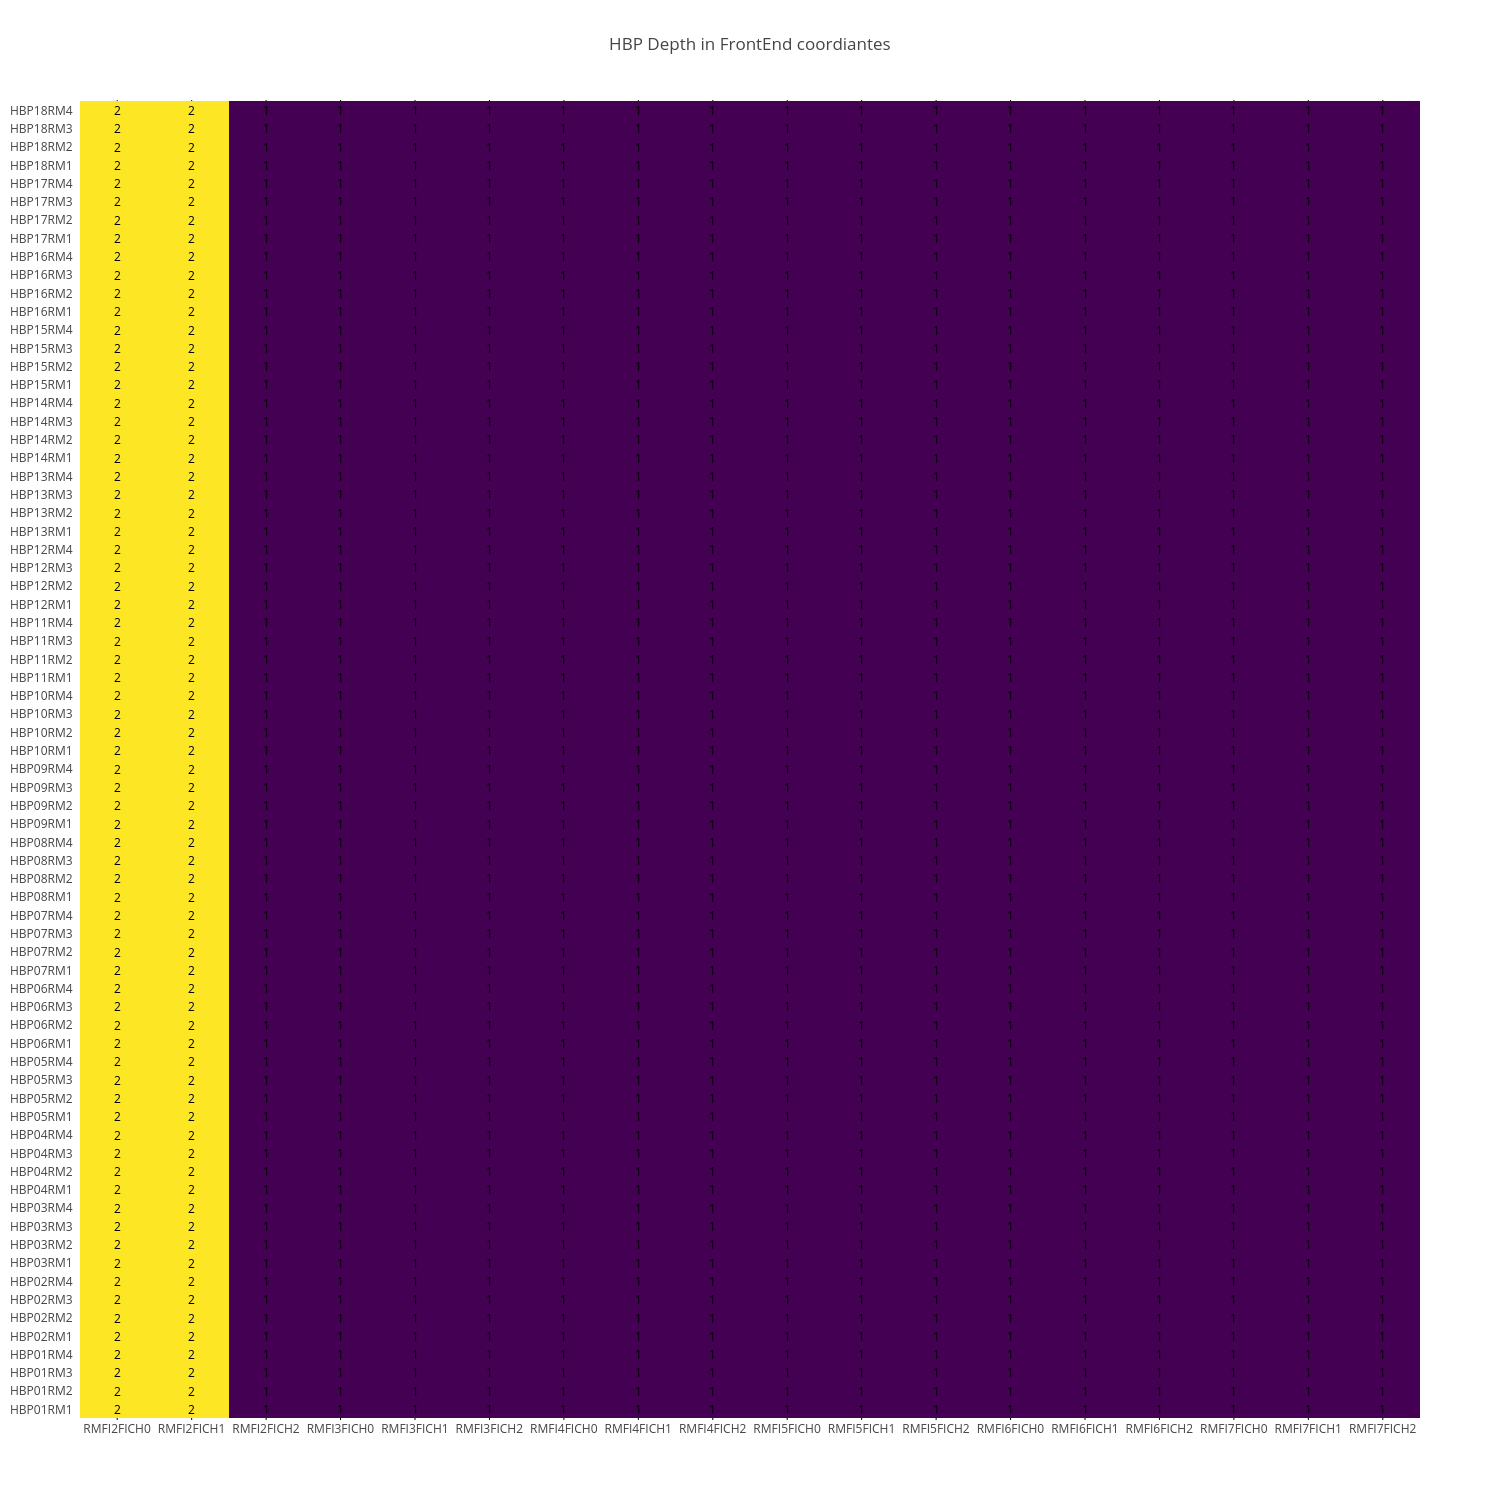
\includegraphics[angle=0,width=0.95\textwidth]{figures/appendix/HBP_Depth_in_FrontEnd.png}
  \end{tabular}
	\caption{HCAL (phase 1 HB, plus side) detector depth distribution in the frontend electronic coordinates.}
  \label{fig:lmapHBPDepthFEC}
 \end{center}
\end{figure}
\clearpage

\begin{figure}[htb]
 \begin{center}
  \begin{tabular}{cc}
   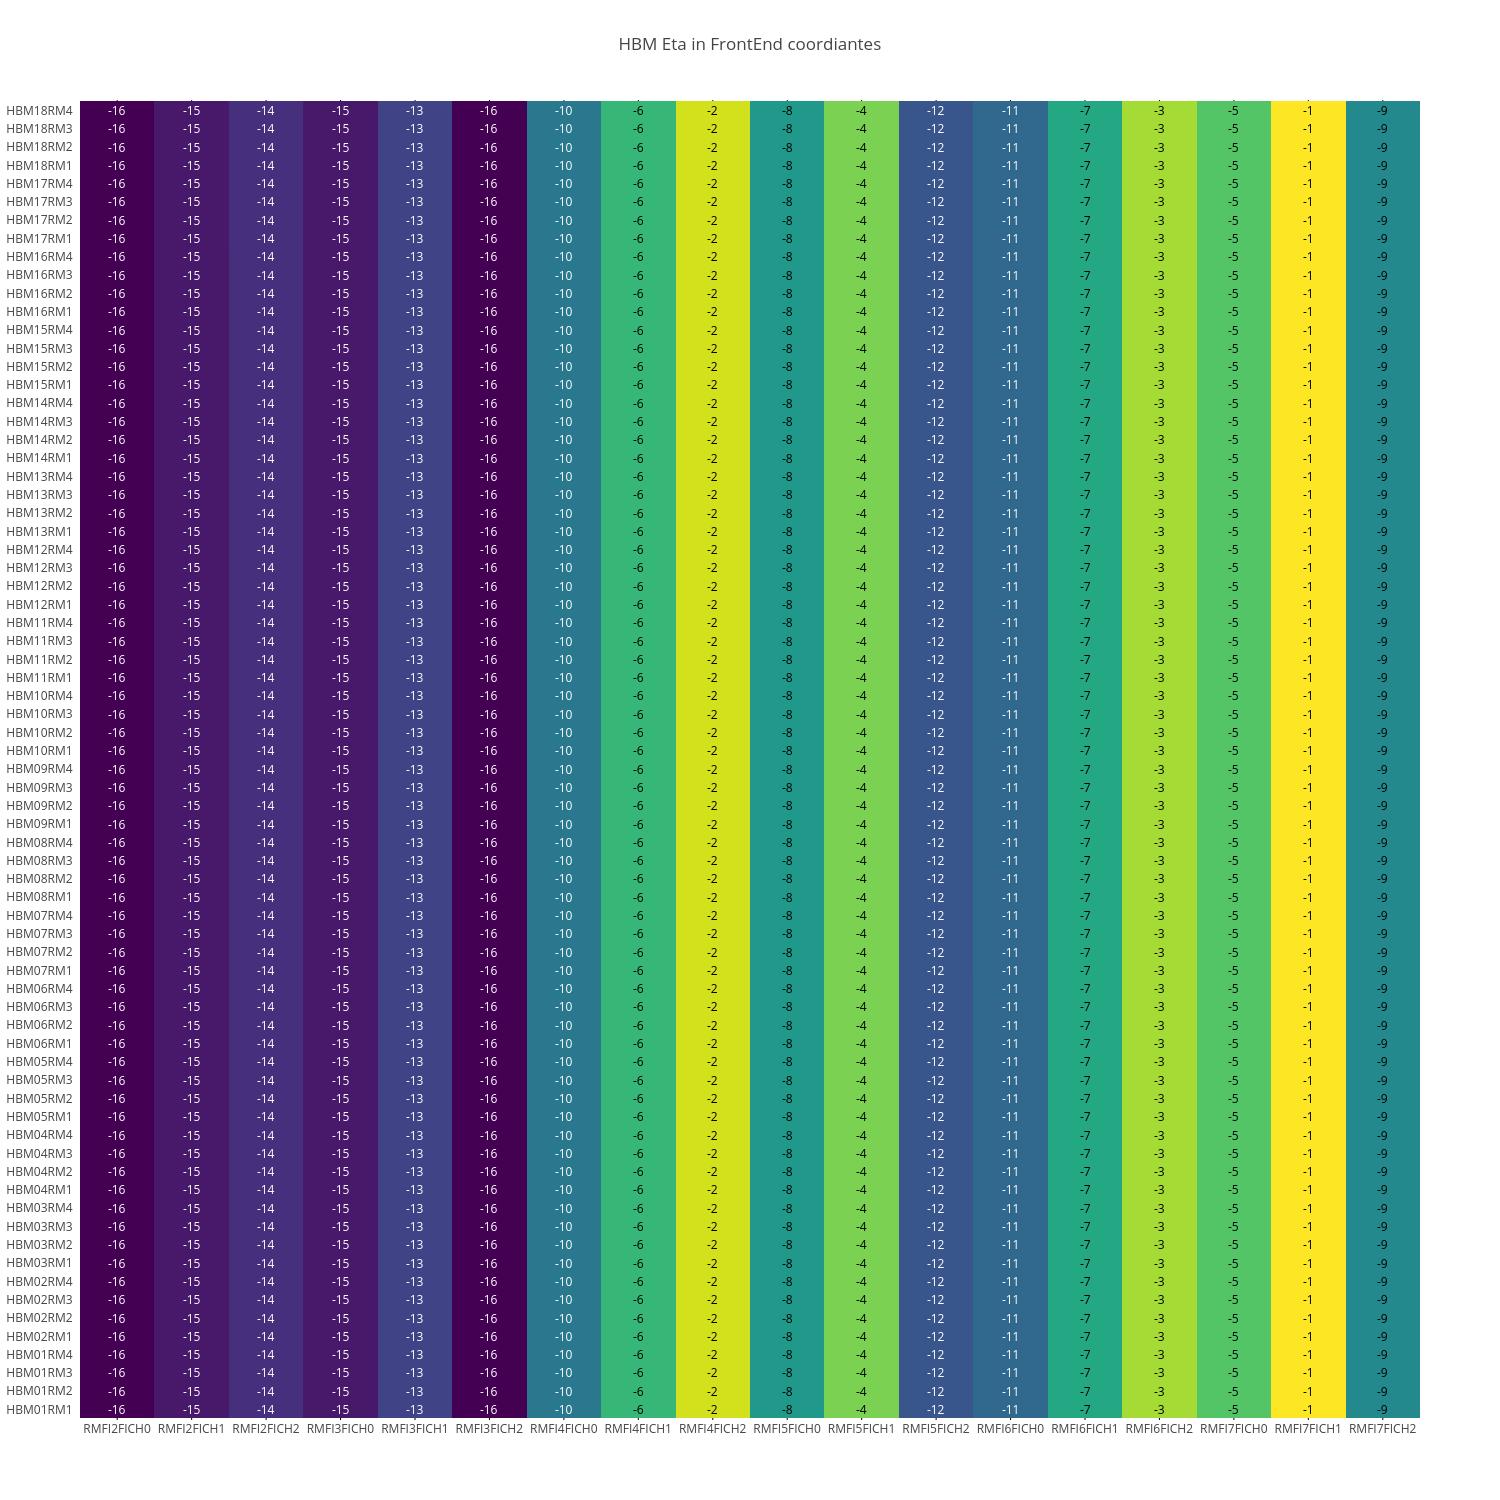
\includegraphics[angle=0,width=0.95\textwidth]{figures/appendix/HBM_Eta_in_FrontEnd.png}
  \end{tabular}
  \caption{HCAL (phase 1 HB, minus side) detector $\eta$ distribution in the frontend electronic coordinates.}
  \label{fig:lmapHBMEtaFEC}
 \end{center}
\end{figure}
\clearpage

\begin{figure}[htb]
 \begin{center}
  \begin{tabular}{cc}
   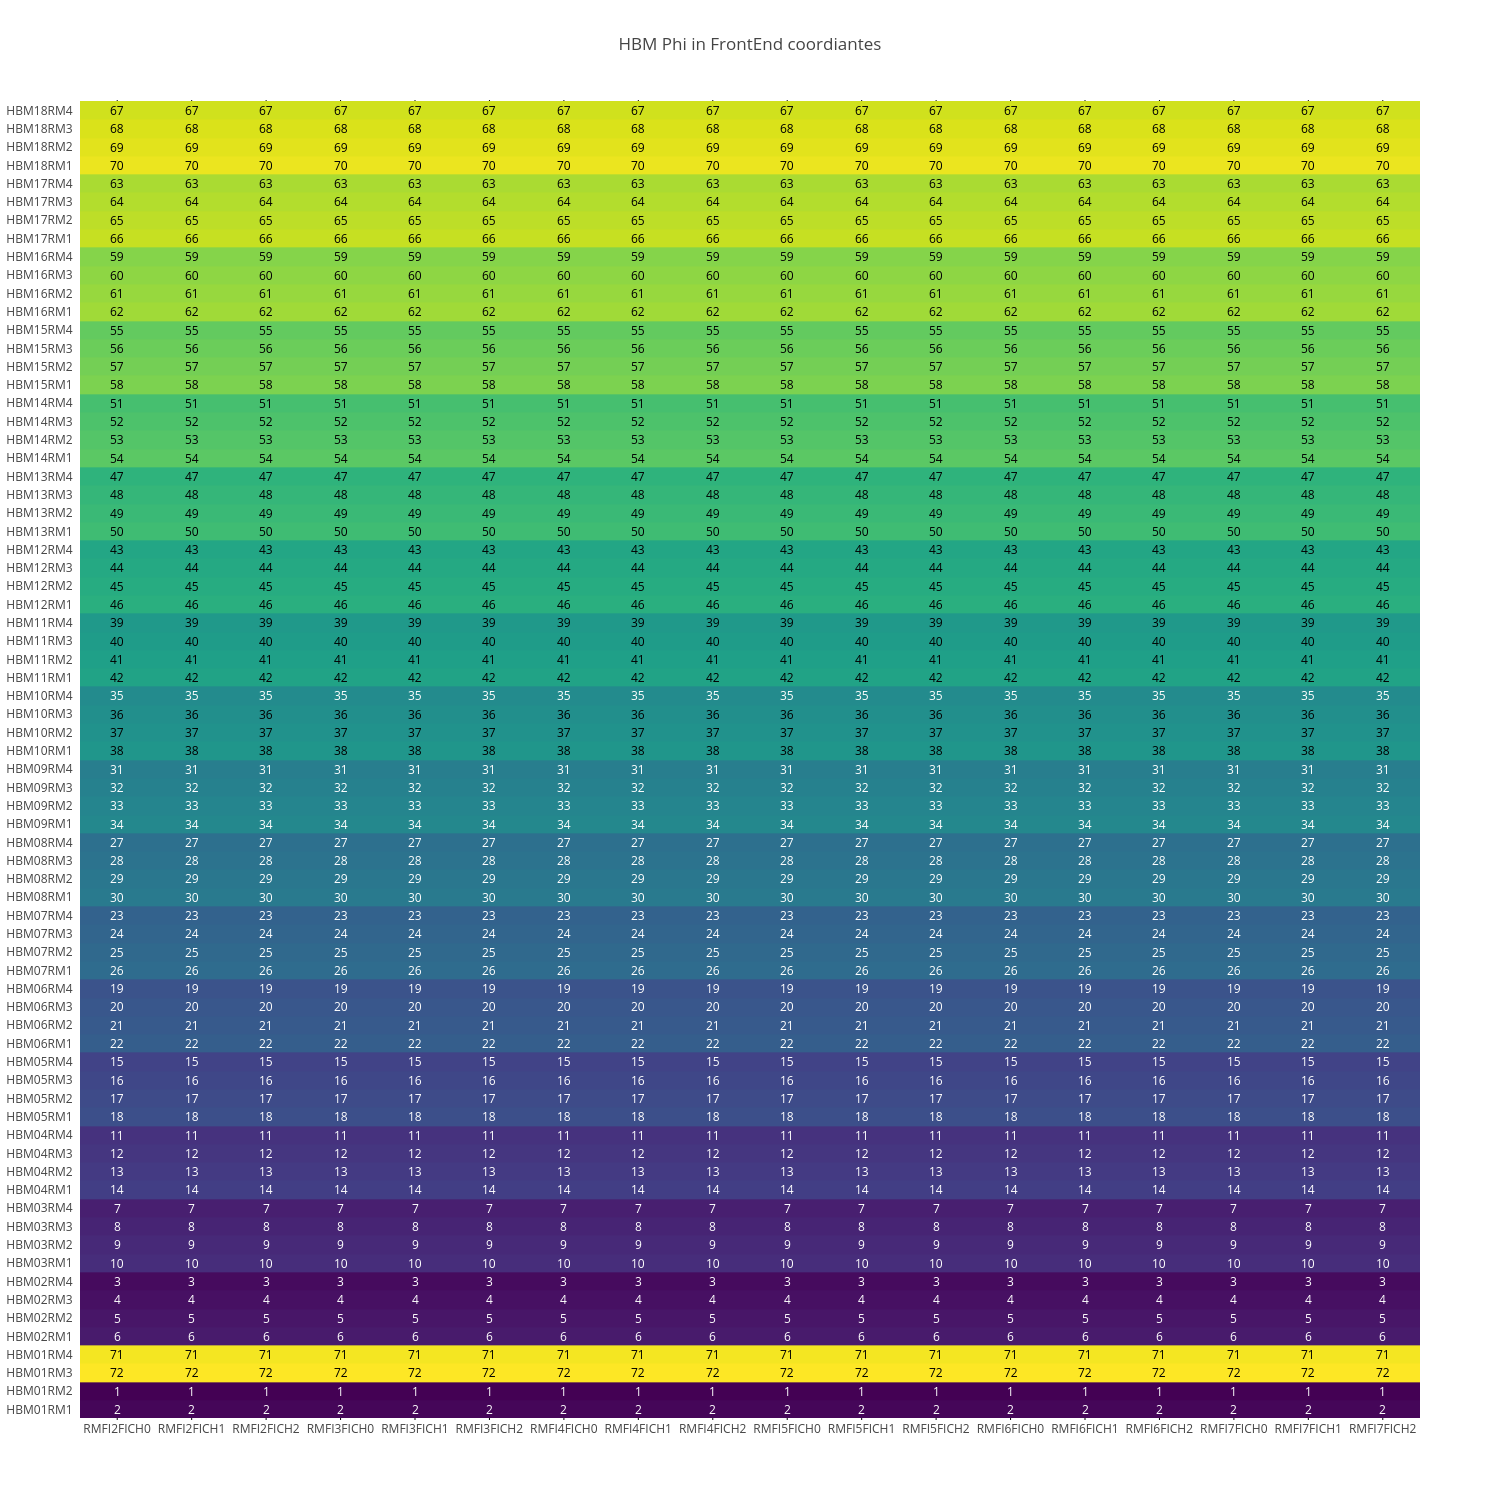
\includegraphics[angle=0,width=0.95\textwidth]{figures/appendix/HBM_Phi_in_FrontEnd.png}
  \end{tabular}
  \caption{HCAL (phase 1 HB, minus side) detector $\phi$ distribution in the frontend electronic coordinates.}
  \label{fig:lmapHBMPhiFEC}
 \end{center}
\end{figure}
\clearpage

\begin{figure}[htb]
 \begin{center}
  \begin{tabular}{cc}
   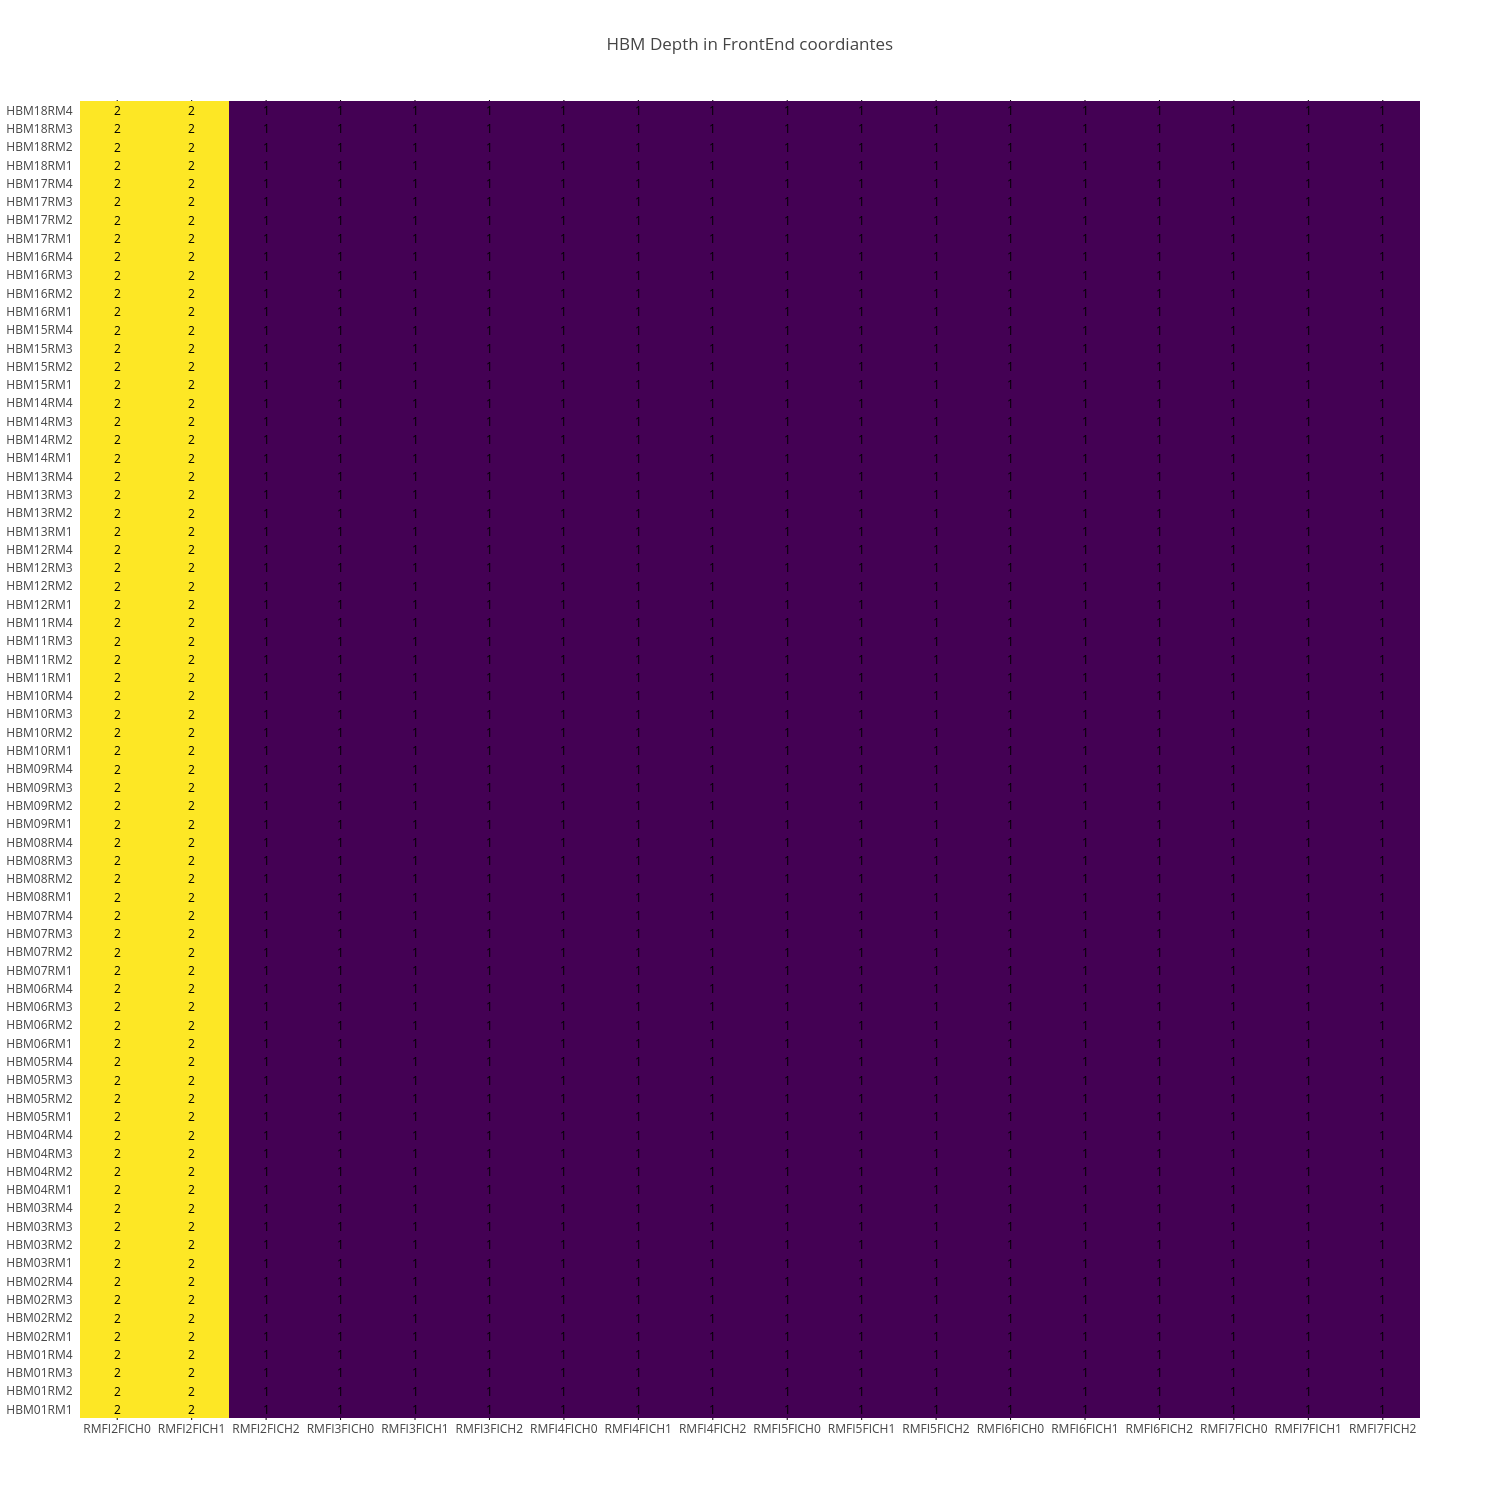
\includegraphics[angle=0,width=0.95\textwidth]{figures/appendix/HBM_Depth_in_FrontEnd.png}
  \end{tabular}
  \caption{HCAL (phase 1 HB, minus side) detector depth distribution in the frontend electronic coordinates.}
  \label{fig:lmapHBMDepthFEC}
 \end{center}
\end{figure}
\clearpage

\begin{figure}[htb]
 \begin{center}
  \begin{tabular}{cc}
   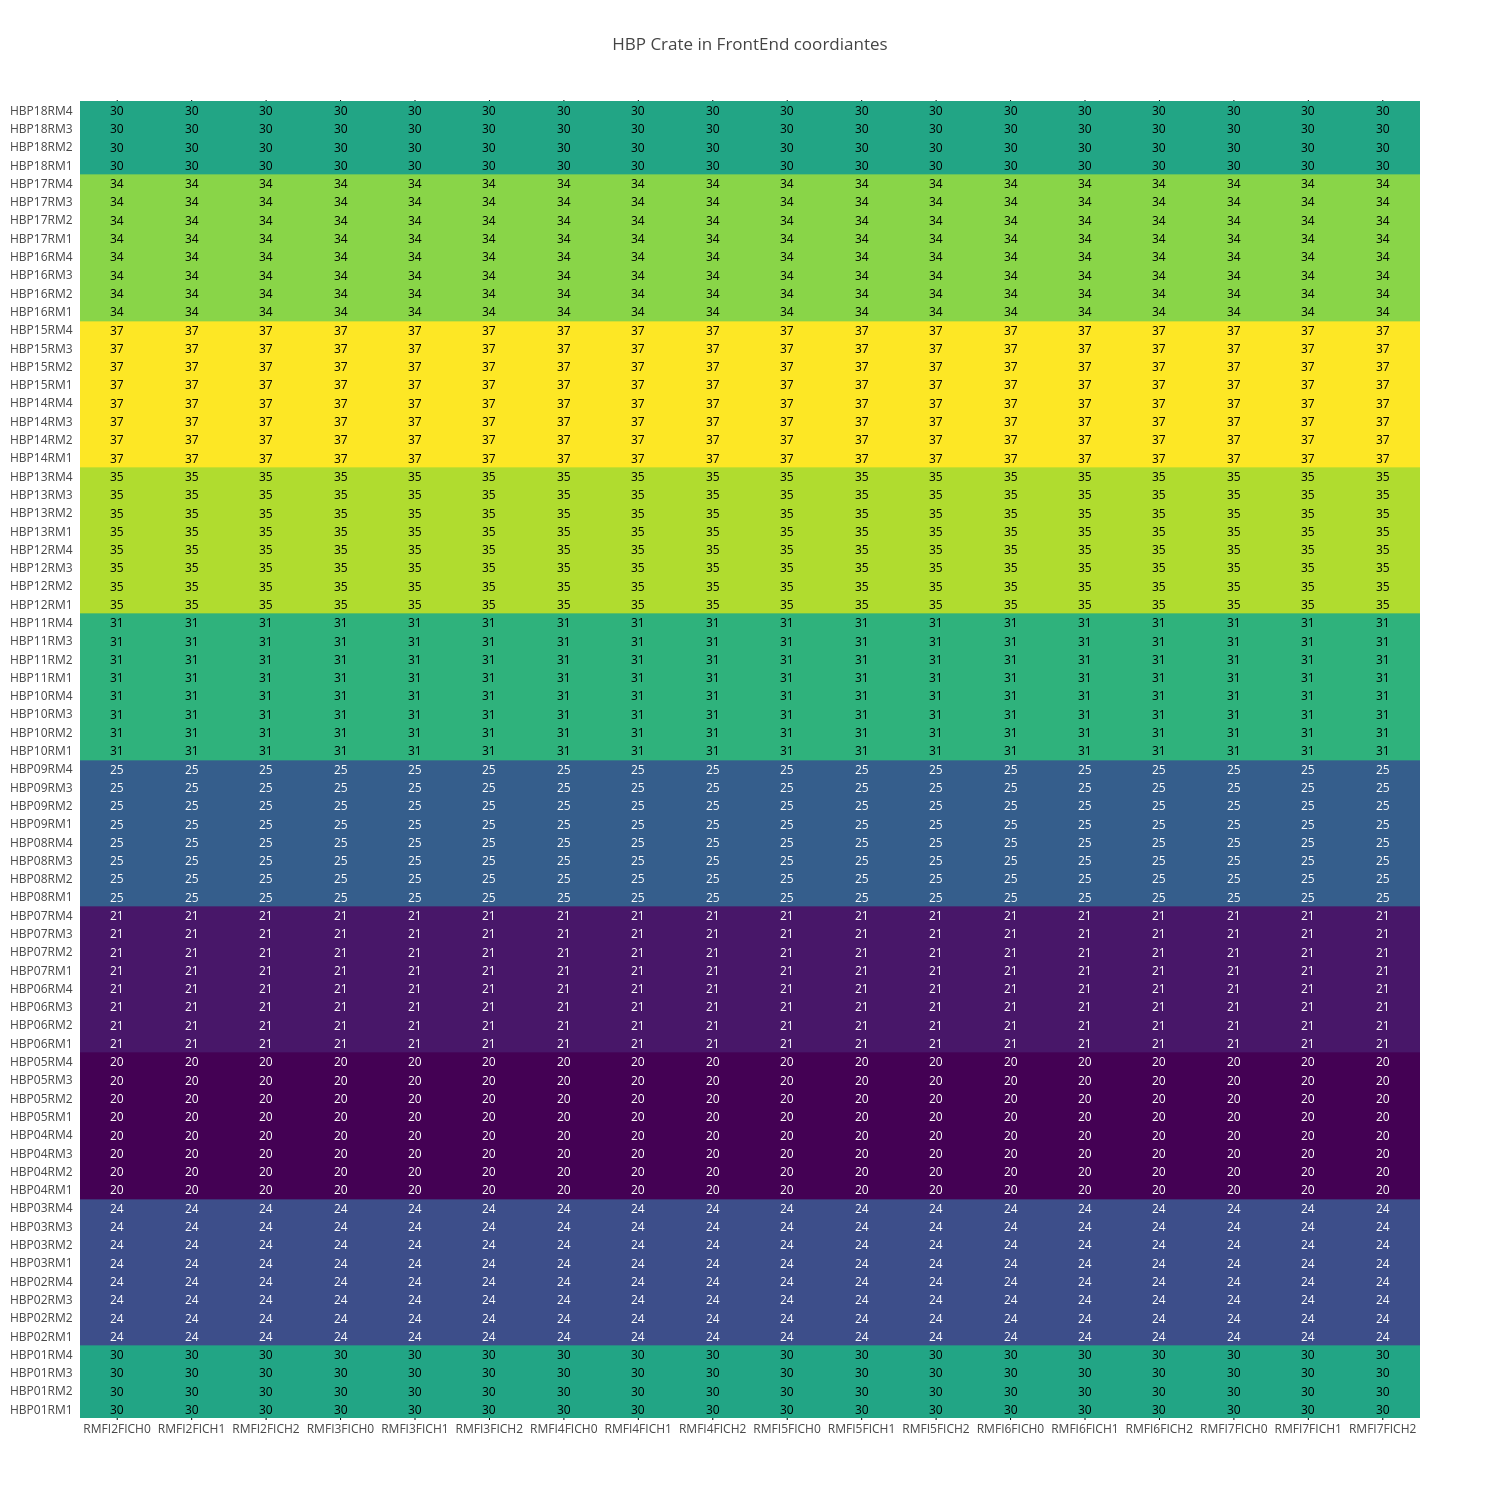
\includegraphics[angle=0,width=0.95\textwidth]{figures/appendix/HBP_Crate_in_FrontEnd.png}
  \end{tabular}
  \caption{HCAL (phase 1 HB, plus side) backend electronic coordinate crate distribution in the frontend electronic coordinates.}
  \label{fig:lmapHBPCrateFEC}
 \end{center}
\end{figure}
\clearpage

\begin{figure}[htb]
 \begin{center}
  \begin{tabular}{cc}
   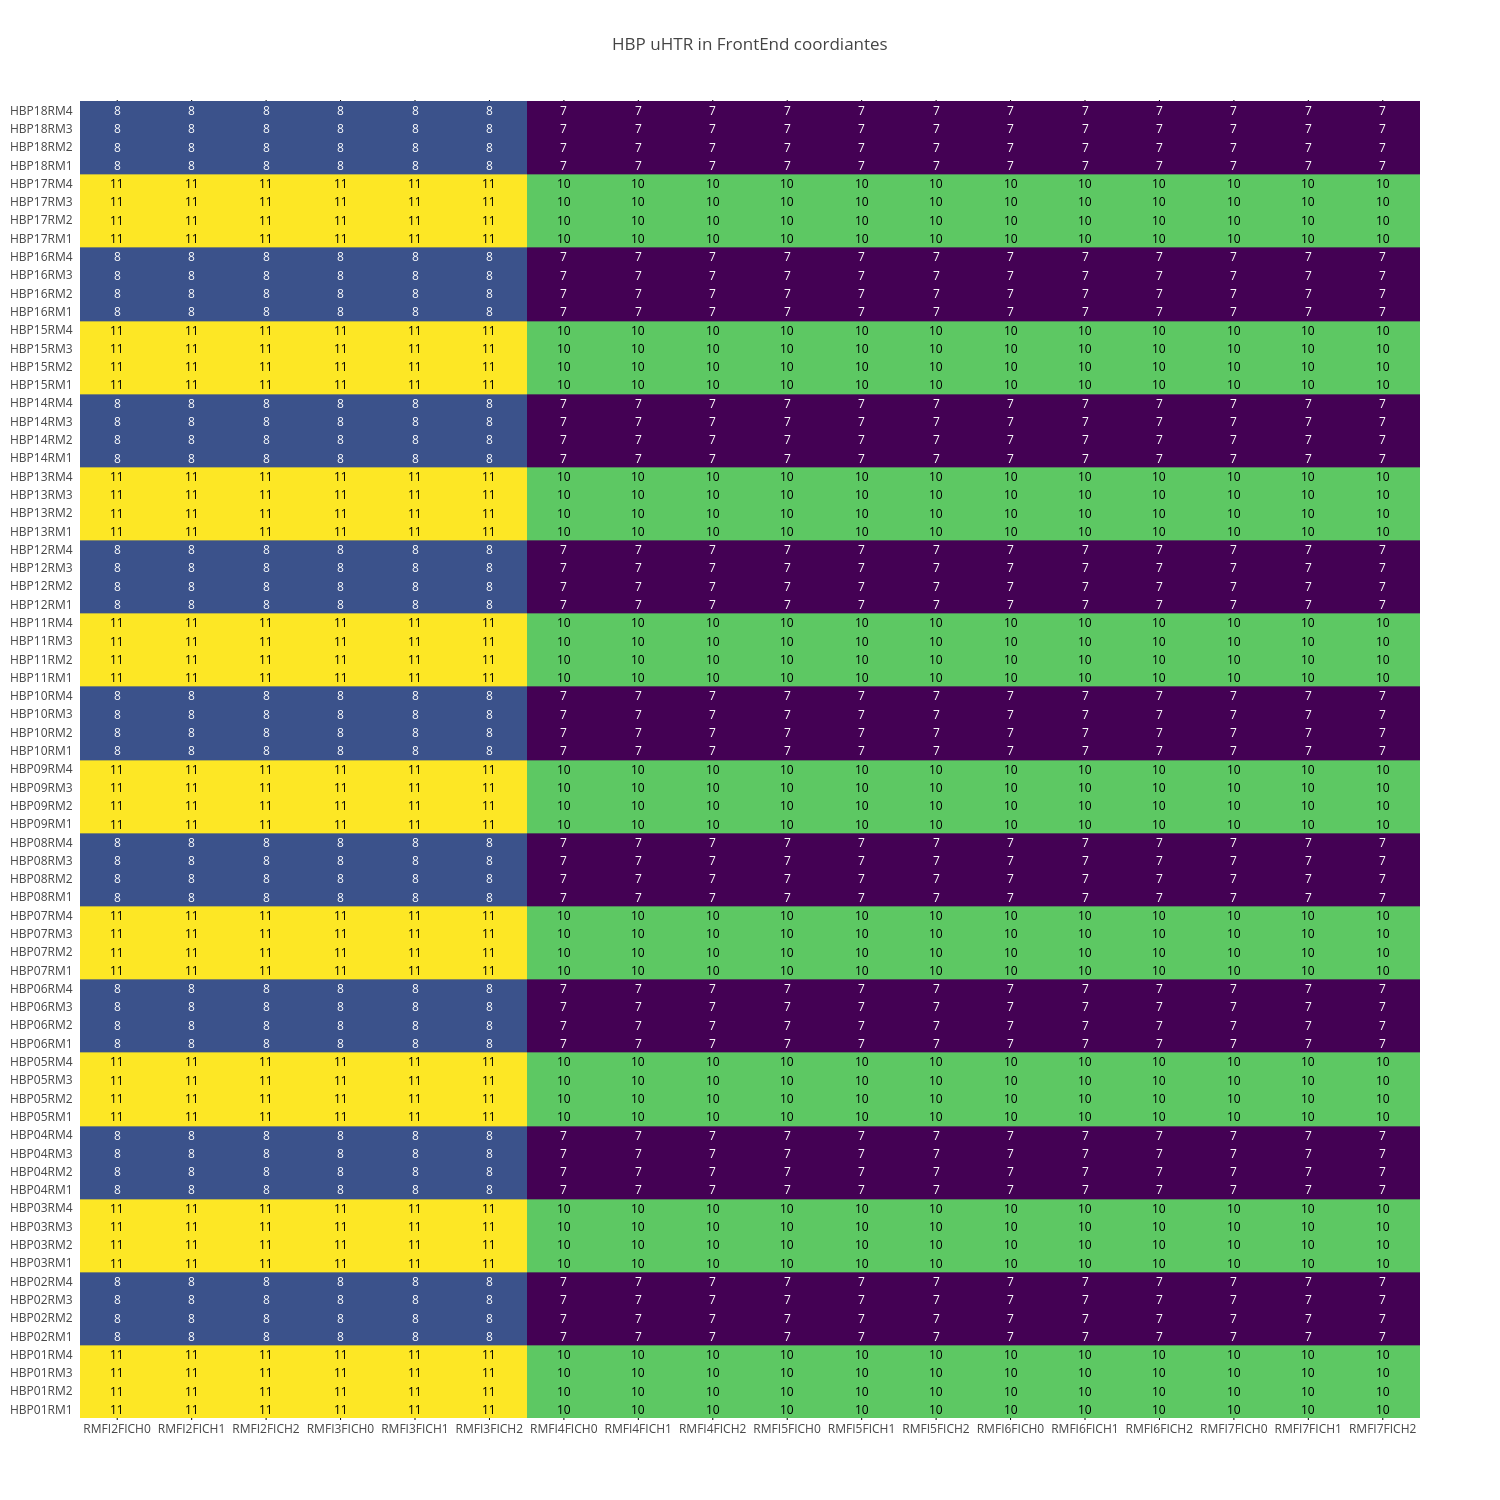
\includegraphics[angle=0,width=0.95\textwidth]{figures/appendix/HBP_uHTR_in_FrontEnd.png}
  \end{tabular}
  \caption{HCAL (phase 1 HB, plus side) backend electronic coordinate uHTR slot distribution in the frontend electronic coordinates.}
  \label{fig:lmapHBPuHTRFEC}
 \end{center}
\end{figure}
\clearpage

\begin{figure}[htb]
 \begin{center}
  \begin{tabular}{cc}
   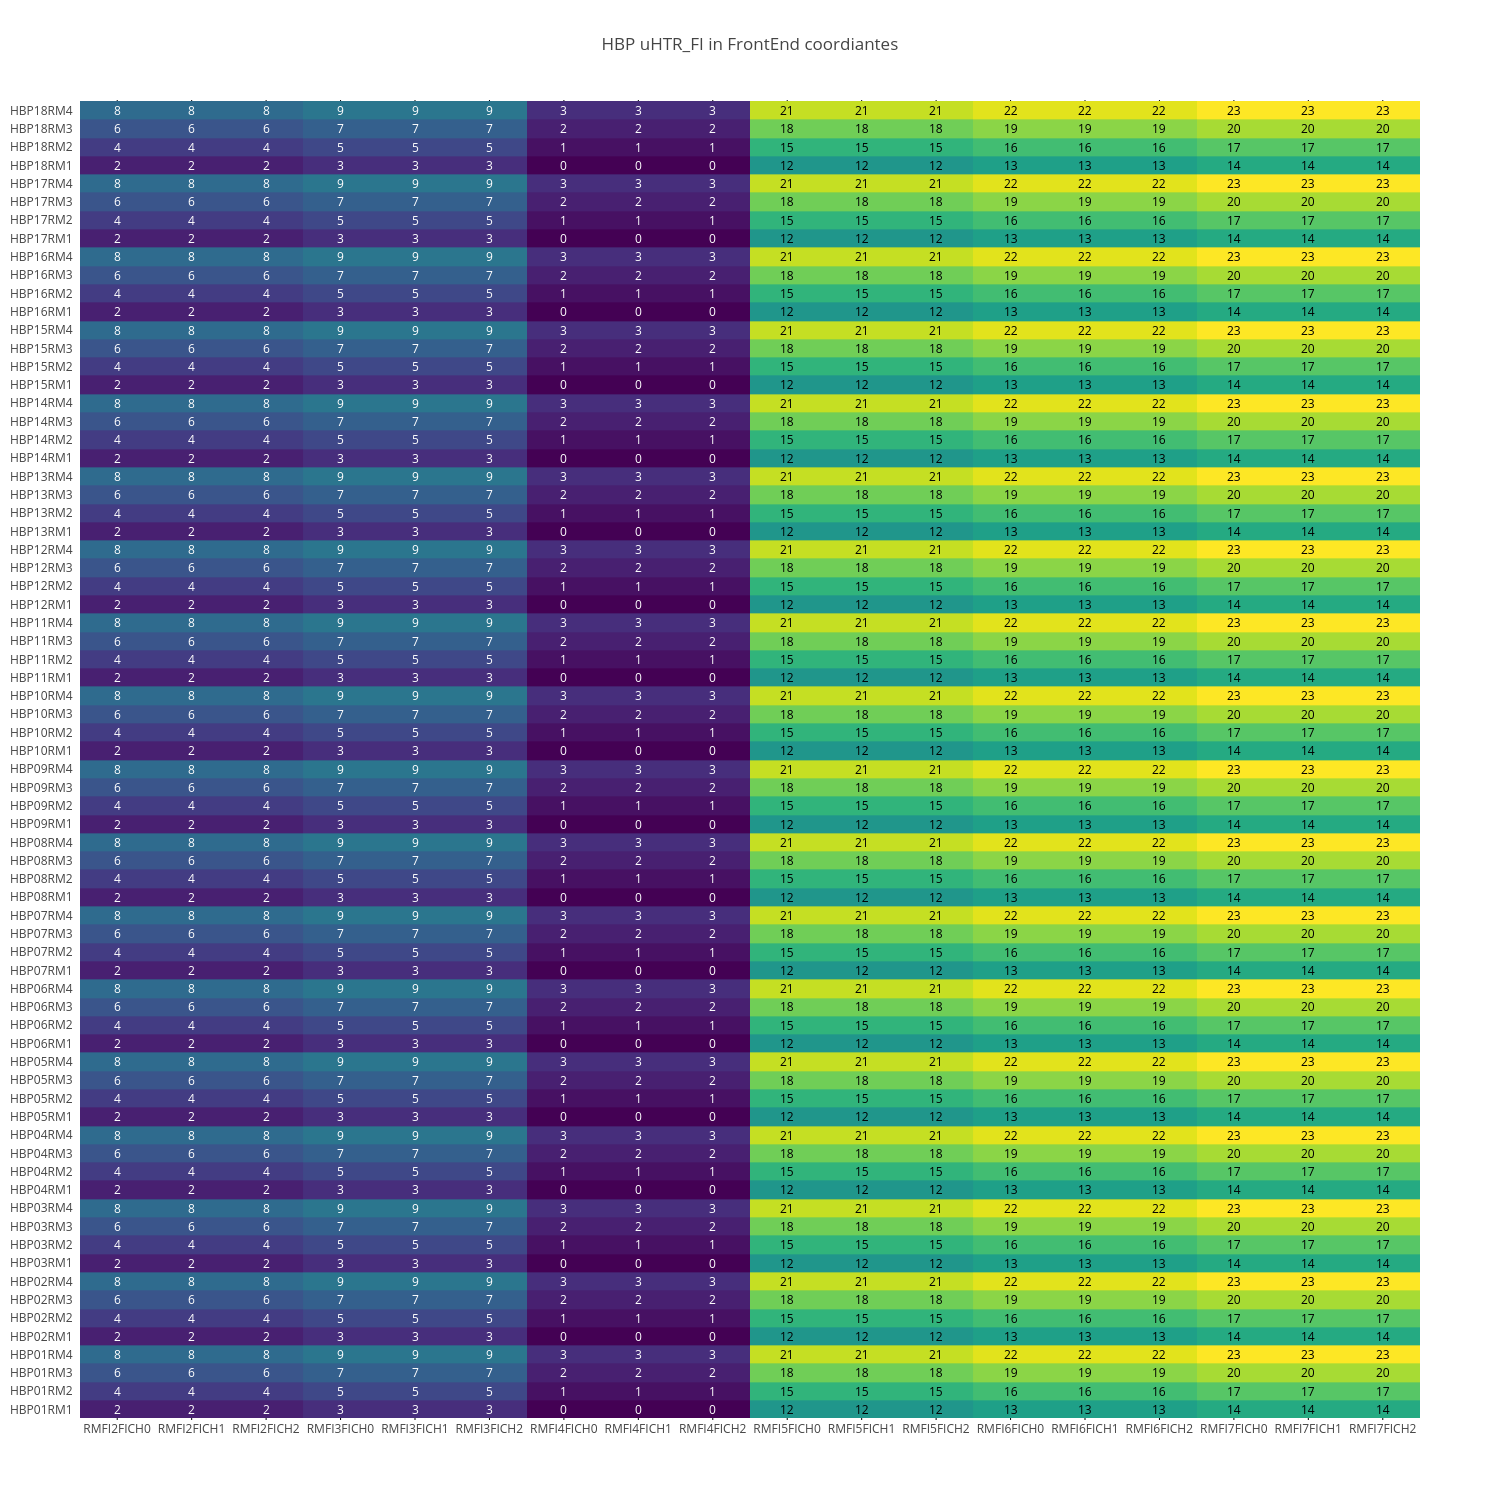
\includegraphics[angle=0,width=0.95\textwidth]{figures/appendix/HBP_uHTR_FI_in_FrontEnd.png}
  \end{tabular}
  \caption{HCAL (phase 1 HB, plus side) backend electronic coordinate uHTR fiber distribution in the frontend electronic coordinates.}
  \label{fig:lmapHBPuHTRFIFEC}
 \end{center}
\end{figure}
\clearpage

\begin{figure}[htb]
 \begin{center}
  \begin{tabular}{cc}
   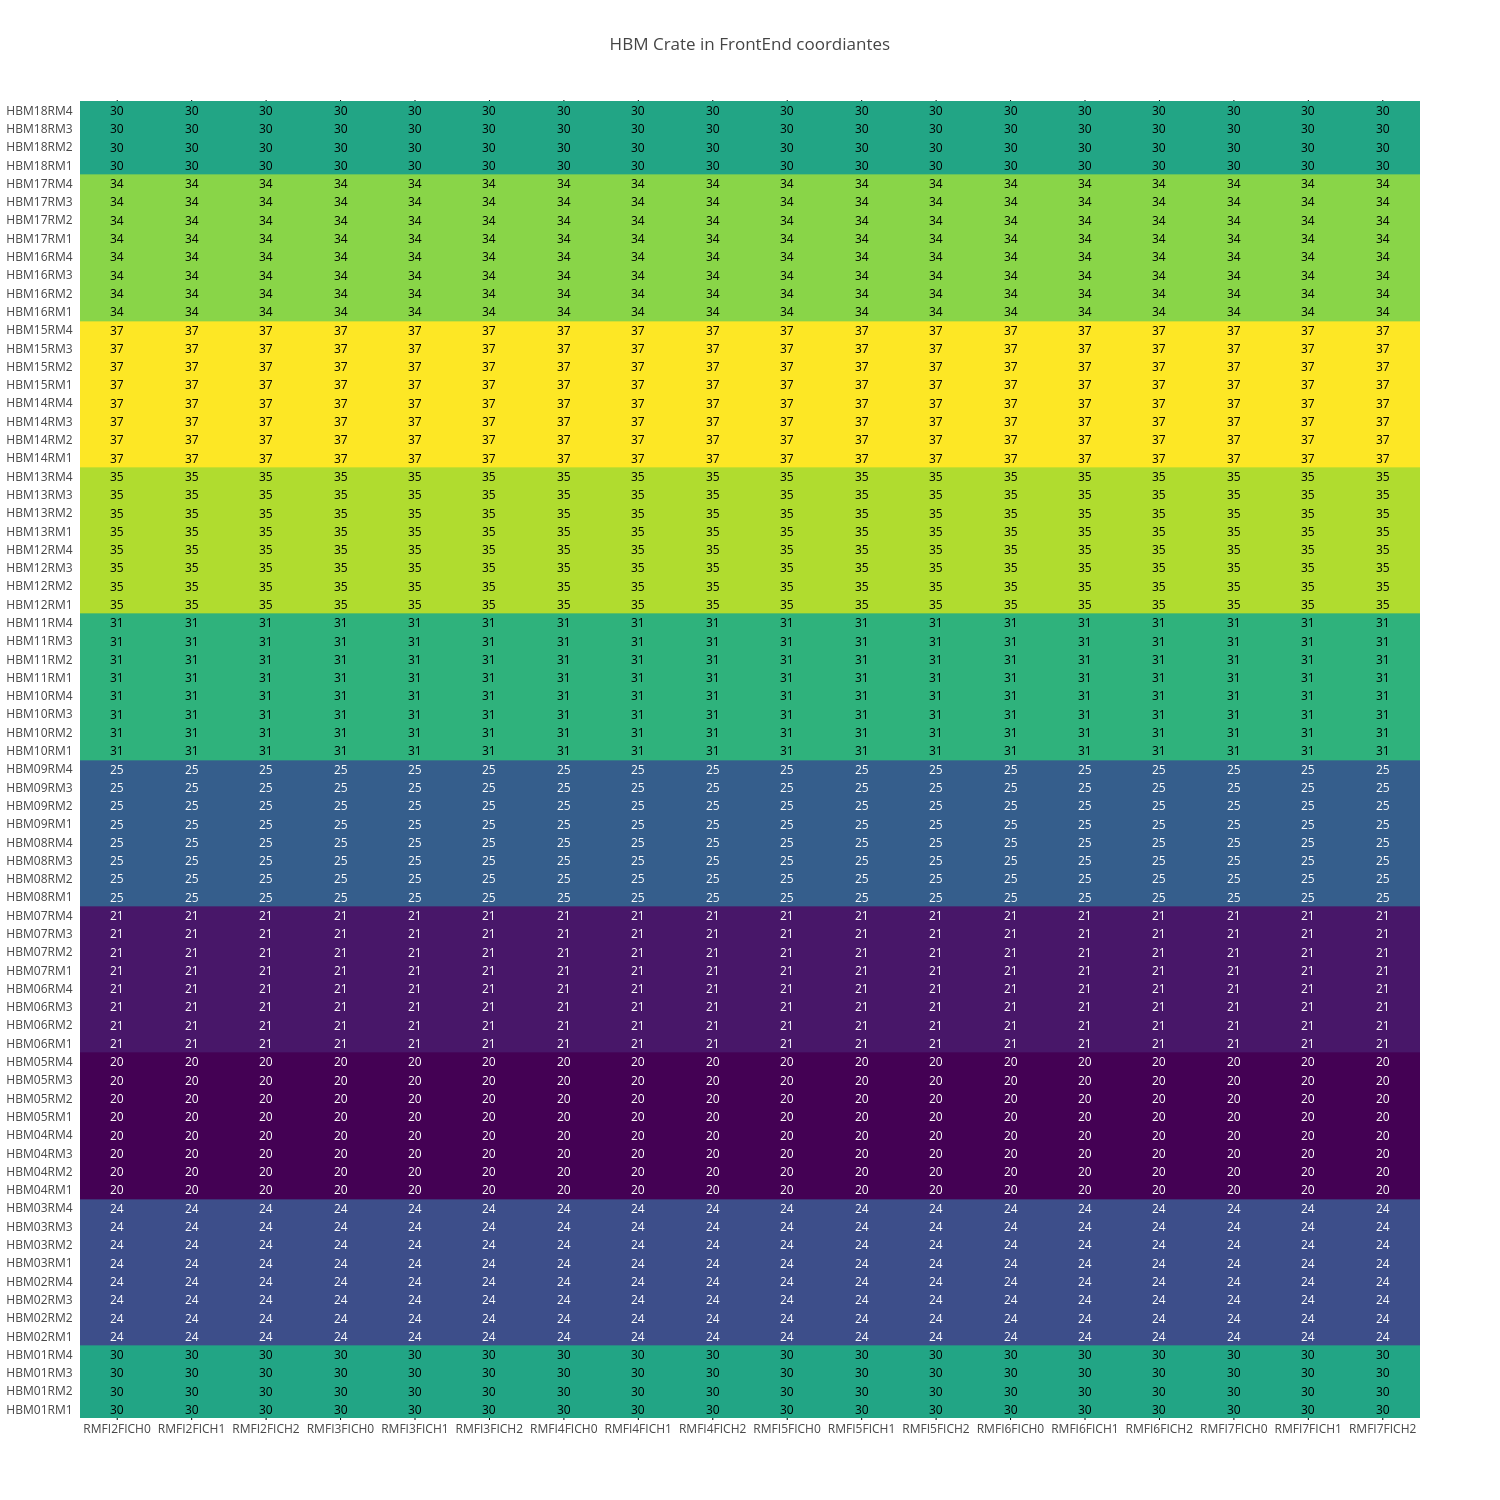
\includegraphics[angle=0,width=0.95\textwidth]{figures/appendix/HBM_Crate_in_FrontEnd.png}
  \end{tabular}
  \caption{HCAL (phase 1 HB, minus side) backend electronic coordinate crate distribution in the frontend electronic coordinates.}
  \label{fig:lmapHBMCrateFEC}
 \end{center}
\end{figure}
\clearpage

\begin{figure}[htb]
 \begin{center}
  \begin{tabular}{cc}
   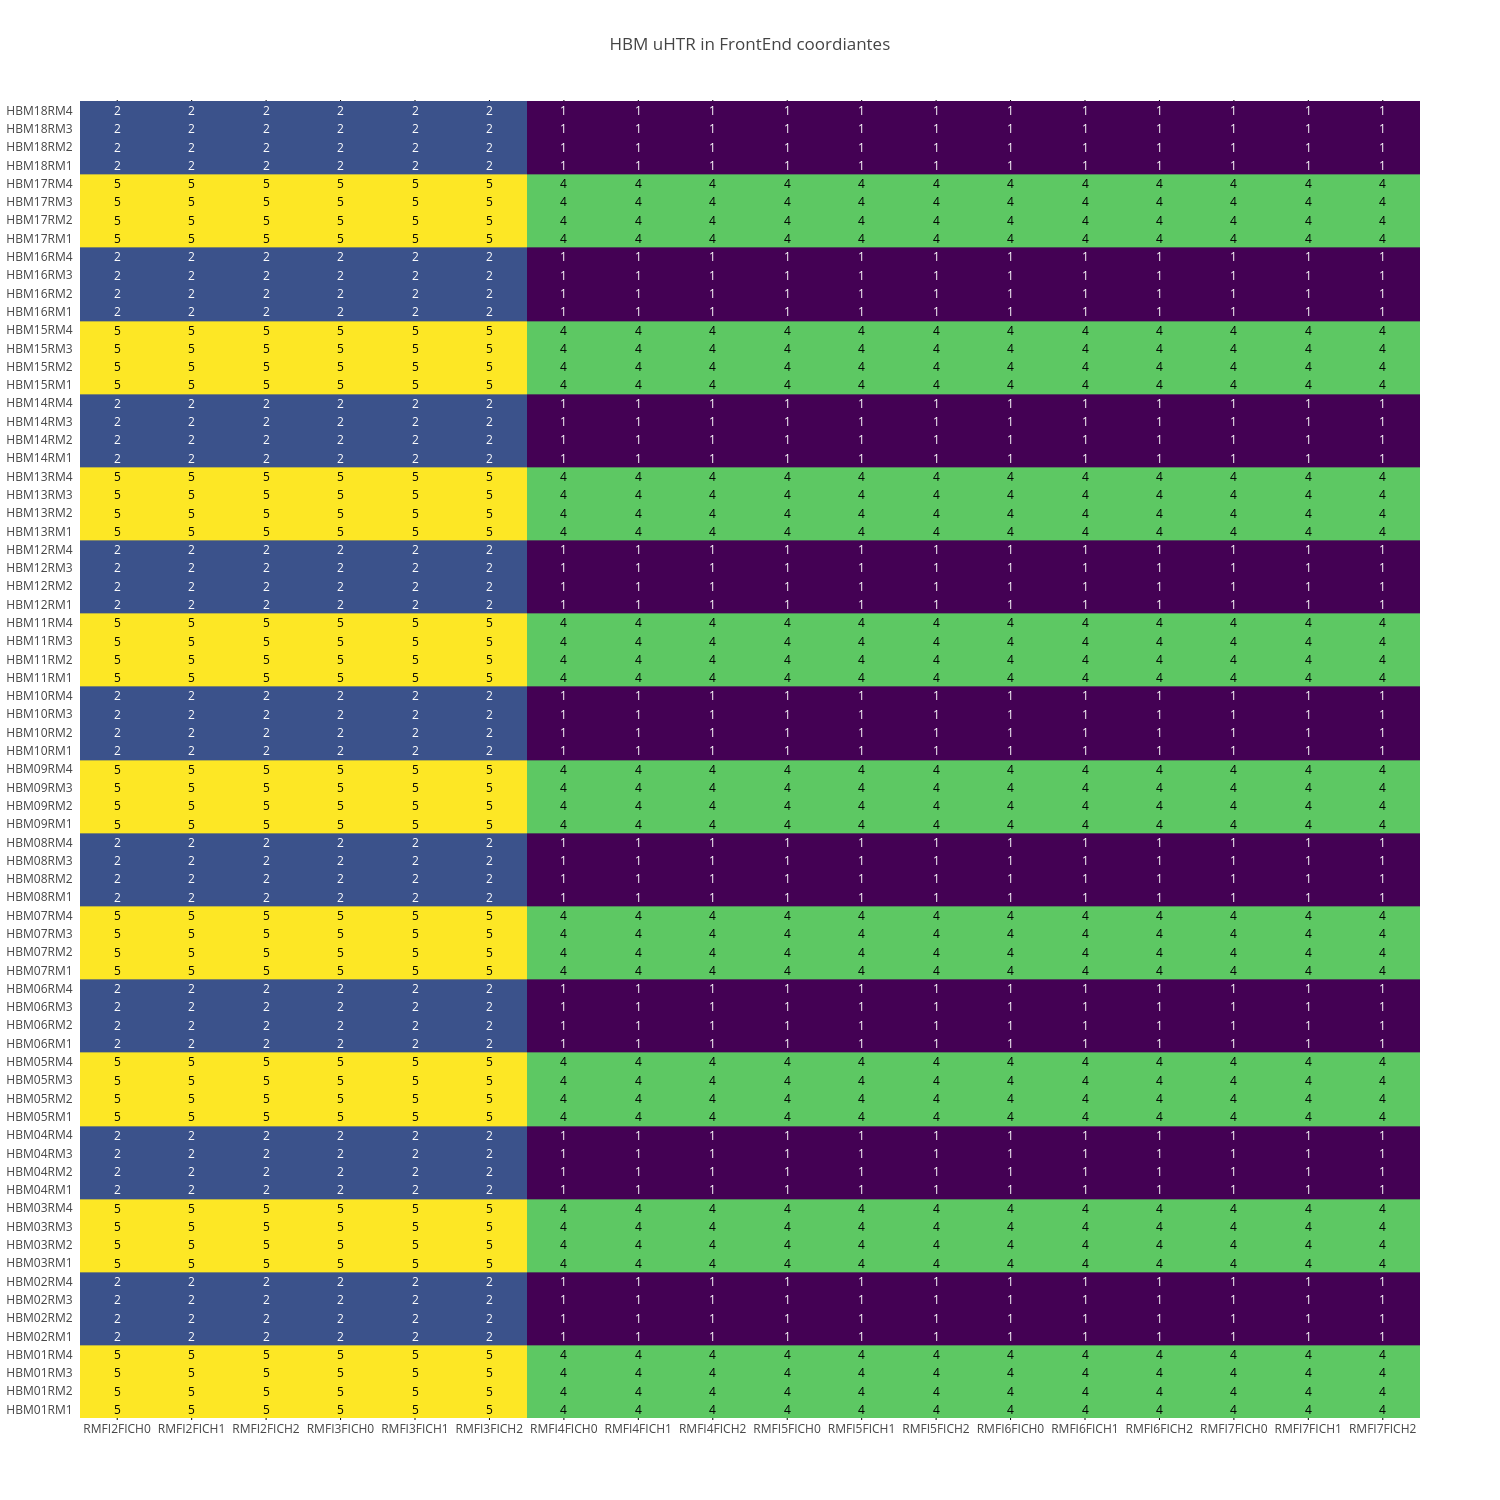
\includegraphics[angle=0,width=0.95\textwidth]{figures/appendix/HBM_uHTR_in_FrontEnd.png}
  \end{tabular}
  \caption{HCAL (phase 1 HB, minus side) backend electronic coordinate uHTR slot distribution in the frontend electronic coordinates.}
  \label{fig:lmapHBMuHTRFEC}
 \end{center}
\end{figure}
\clearpage

\begin{figure}[htb]
 \begin{center}
  \begin{tabular}{cc}
   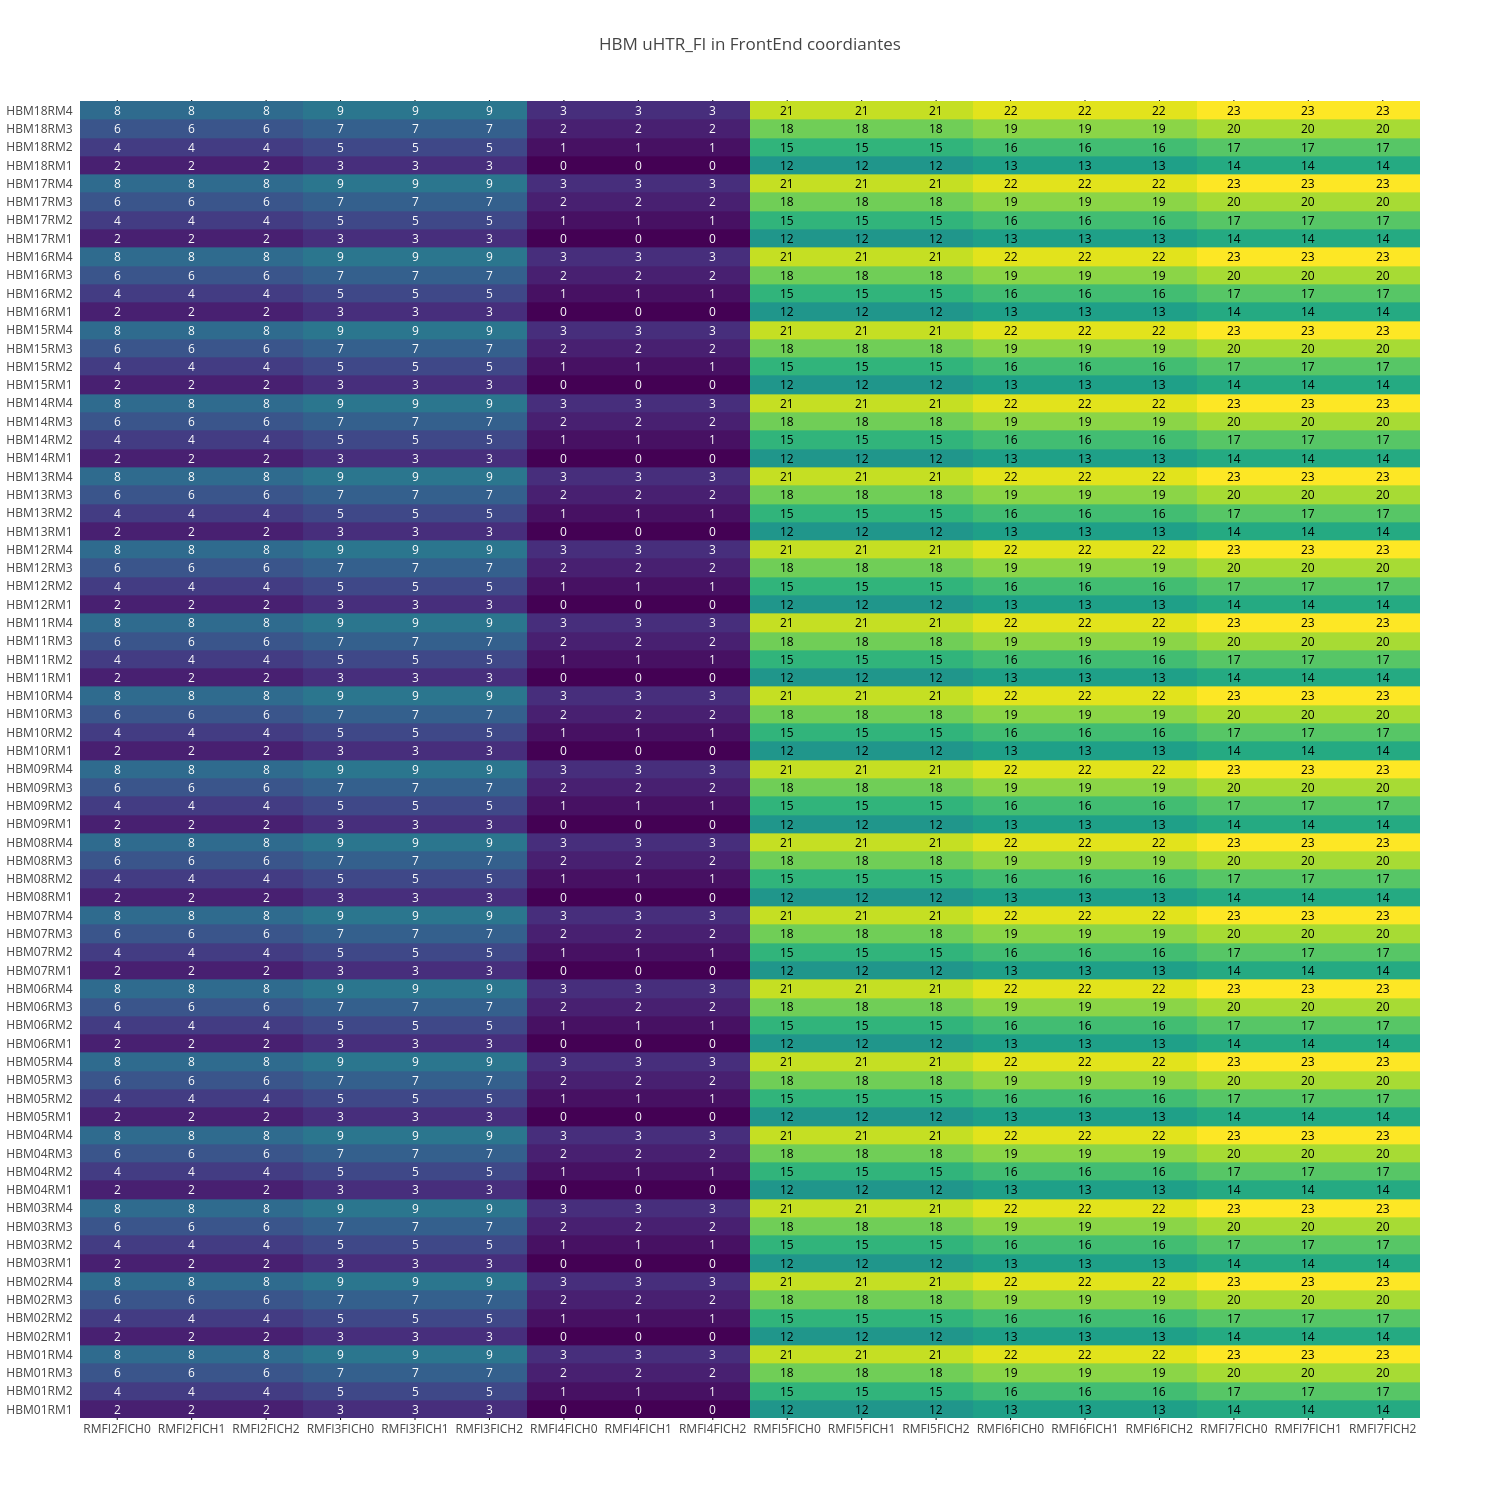
\includegraphics[angle=0,width=0.95\textwidth]{figures/appendix/HBM_uHTR_FI_in_FrontEnd.png}
  \end{tabular}
  \caption{HCAL (phase 1 HB, minus side) backend electronic coordinate uHTR fiber distribution in the frontend electronic coordinates.}
  \label{fig:lmapHBMuHTRFIFEC}
 \end{center}
\end{figure}
\clearpage

\subsection{Phase 2 HB in 2020}
The 2018 HB will be replaced and move to SiPM+QIE11 FrontEnd+uTCA BackEnd stage in 2020, during the long shutdown 2. A complicate swap scheme is applied inside the FrontEnd board to satisfy the trigger latency requirement. Fortunately, thanks to Dick’s elegant design, we do not need to unplug HE fibers from patch panel to fit in the new 2020 HB.

The phase 2 2020 HB validation plots are shown from Fig~\ref{fig:lmapngHBPEtaFEC} to Fig~\ref{fig:lmapngHBMuHTRFIFEC}. There are 9216 readout channels in phase 2 HB. 9072 channels are physical readout channel, corresponding to actual tower and layer on detector. 144 of them are dummy calibration channels, which are readout by FrontEnd with no corresponding detector components. Those dummy calibration channels are labeled as ``HBX" channels. HBX channels are distributed among 144 HB readout modules, but only on two locations: RM fiber 2 fiber channel 2 and RM fiber 3 fiber channel 6. BackEnd electronics are still in 12 uHTR and 24 uHTR fibers, but number of fiber channels per fiber is increased from 3 to 8, to accommodating more readout channels, comparing with 2018 remapped HB.
\clearpage

\begin{figure}[htb]
 \begin{center}
  \begin{tabular}{cc}
   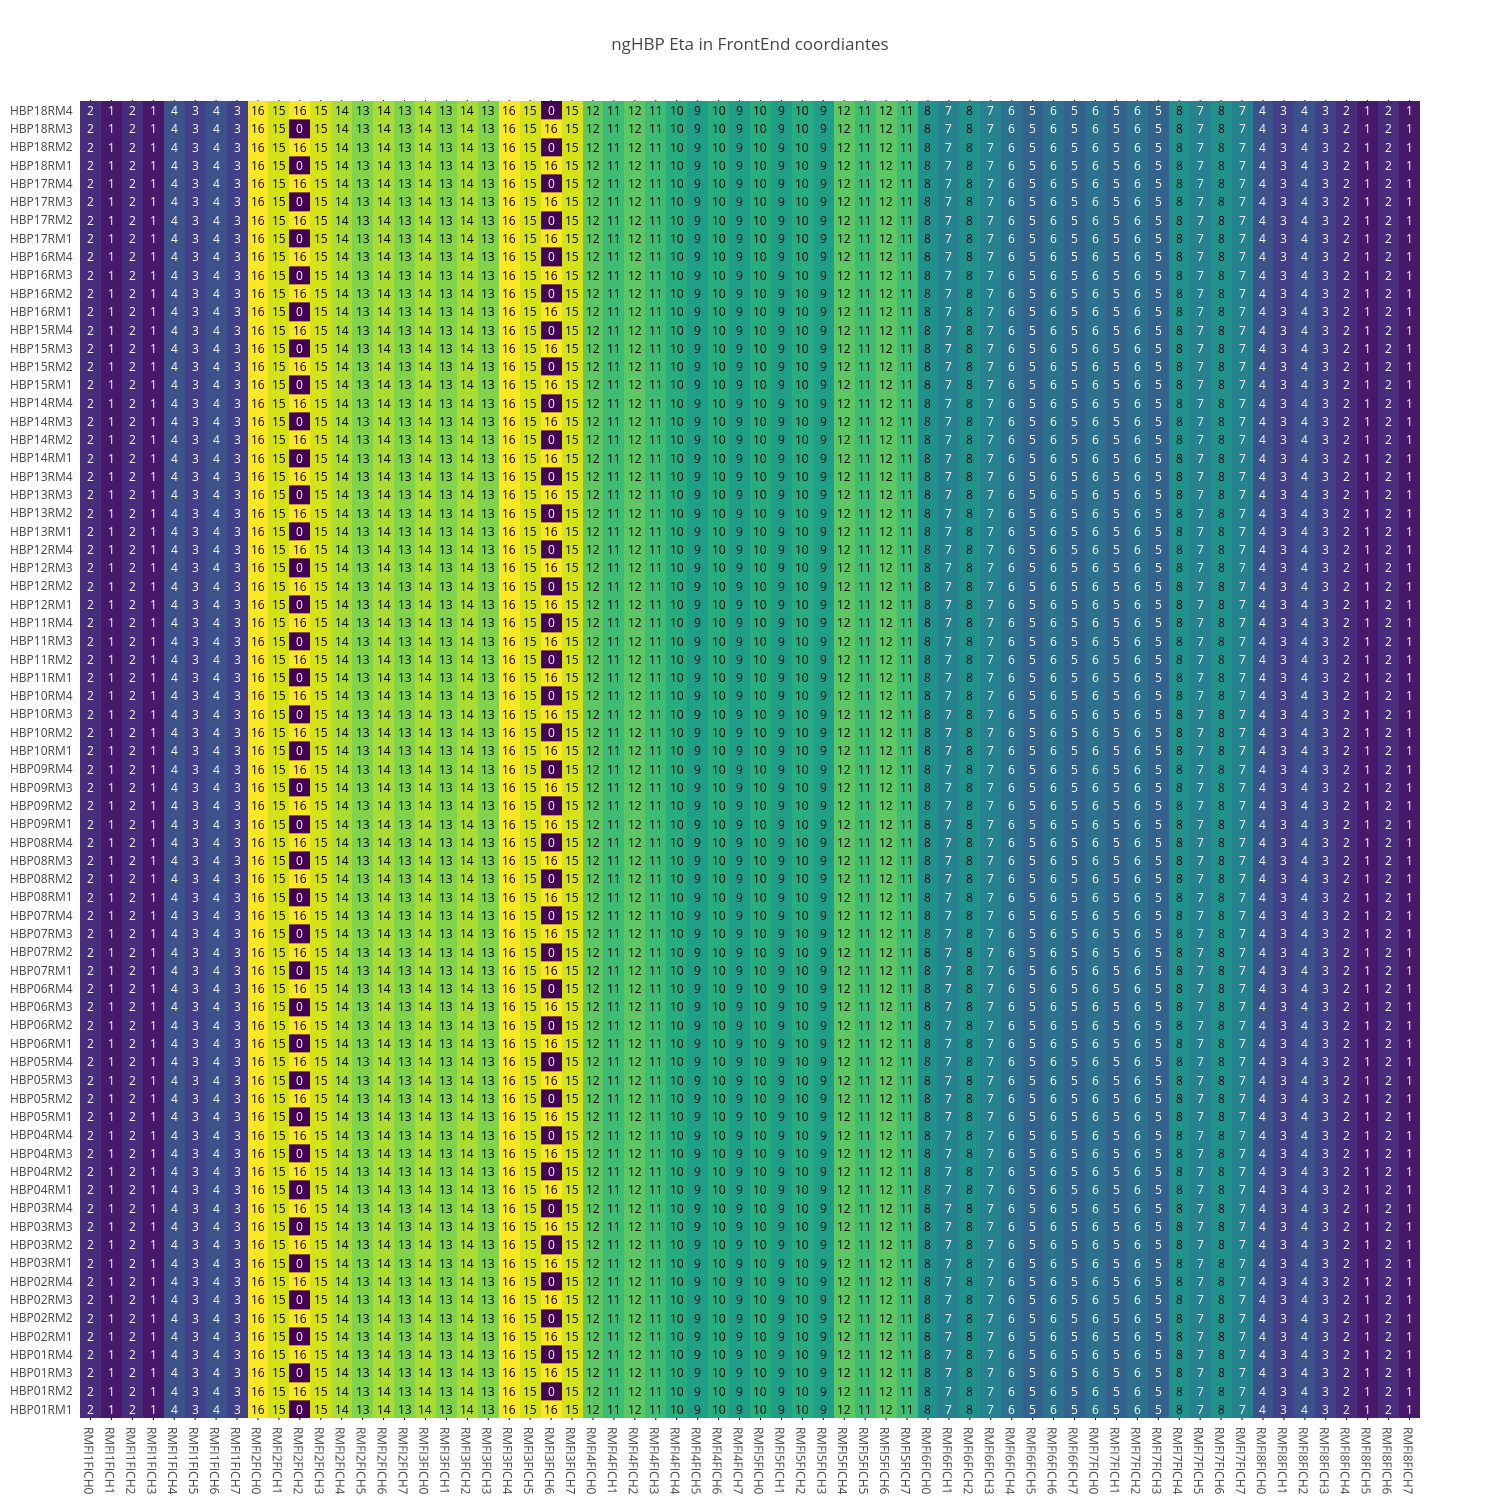
\includegraphics[angle=0,width=0.95\textwidth]{figures/appendix/ngHBP_Eta_in_FrontEnd.png}
  \end{tabular}
	\caption{HCAL (phase 2 HB, plus side) detector $\eta$ distribution in the frontend electronic coordinates.}
  \label{fig:lmapngHBPEtaFEC}
 \end{center}
\end{figure}
\clearpage

\begin{figure}[htb]
 \begin{center}
  \begin{tabular}{cc}
   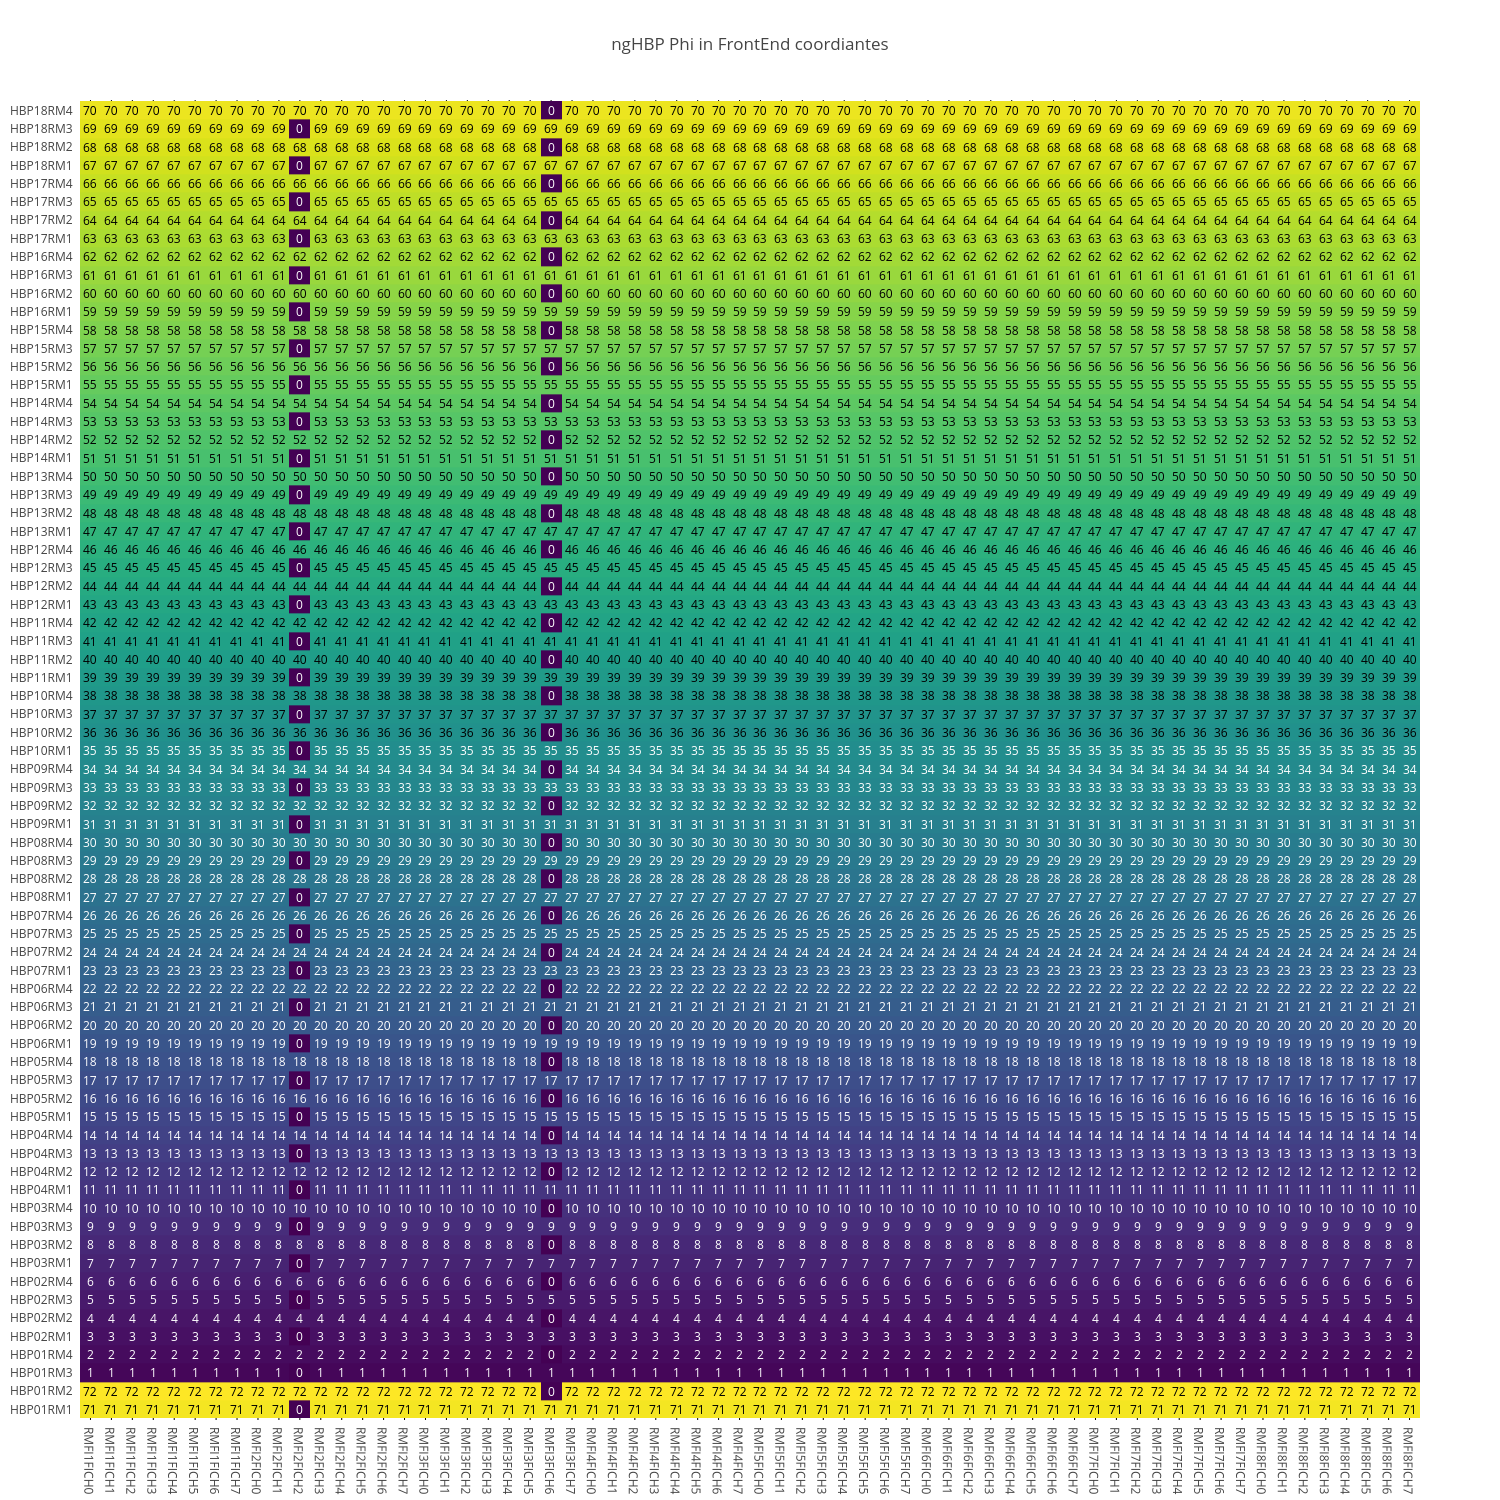
\includegraphics[angle=0,width=0.95\textwidth]{figures/appendix/ngHBP_Phi_in_FrontEnd.png}
  \end{tabular}
	\caption{HCAL (phase 2 HB, plus side) detector $\phi$ distribution in the frontend electronic coordinates.}
  \label{fig:lmapngHBPPhiFEC}
 \end{center}
\end{figure}
\clearpage

\begin{figure}[htb]
 \begin{center}
  \begin{tabular}{cc}
   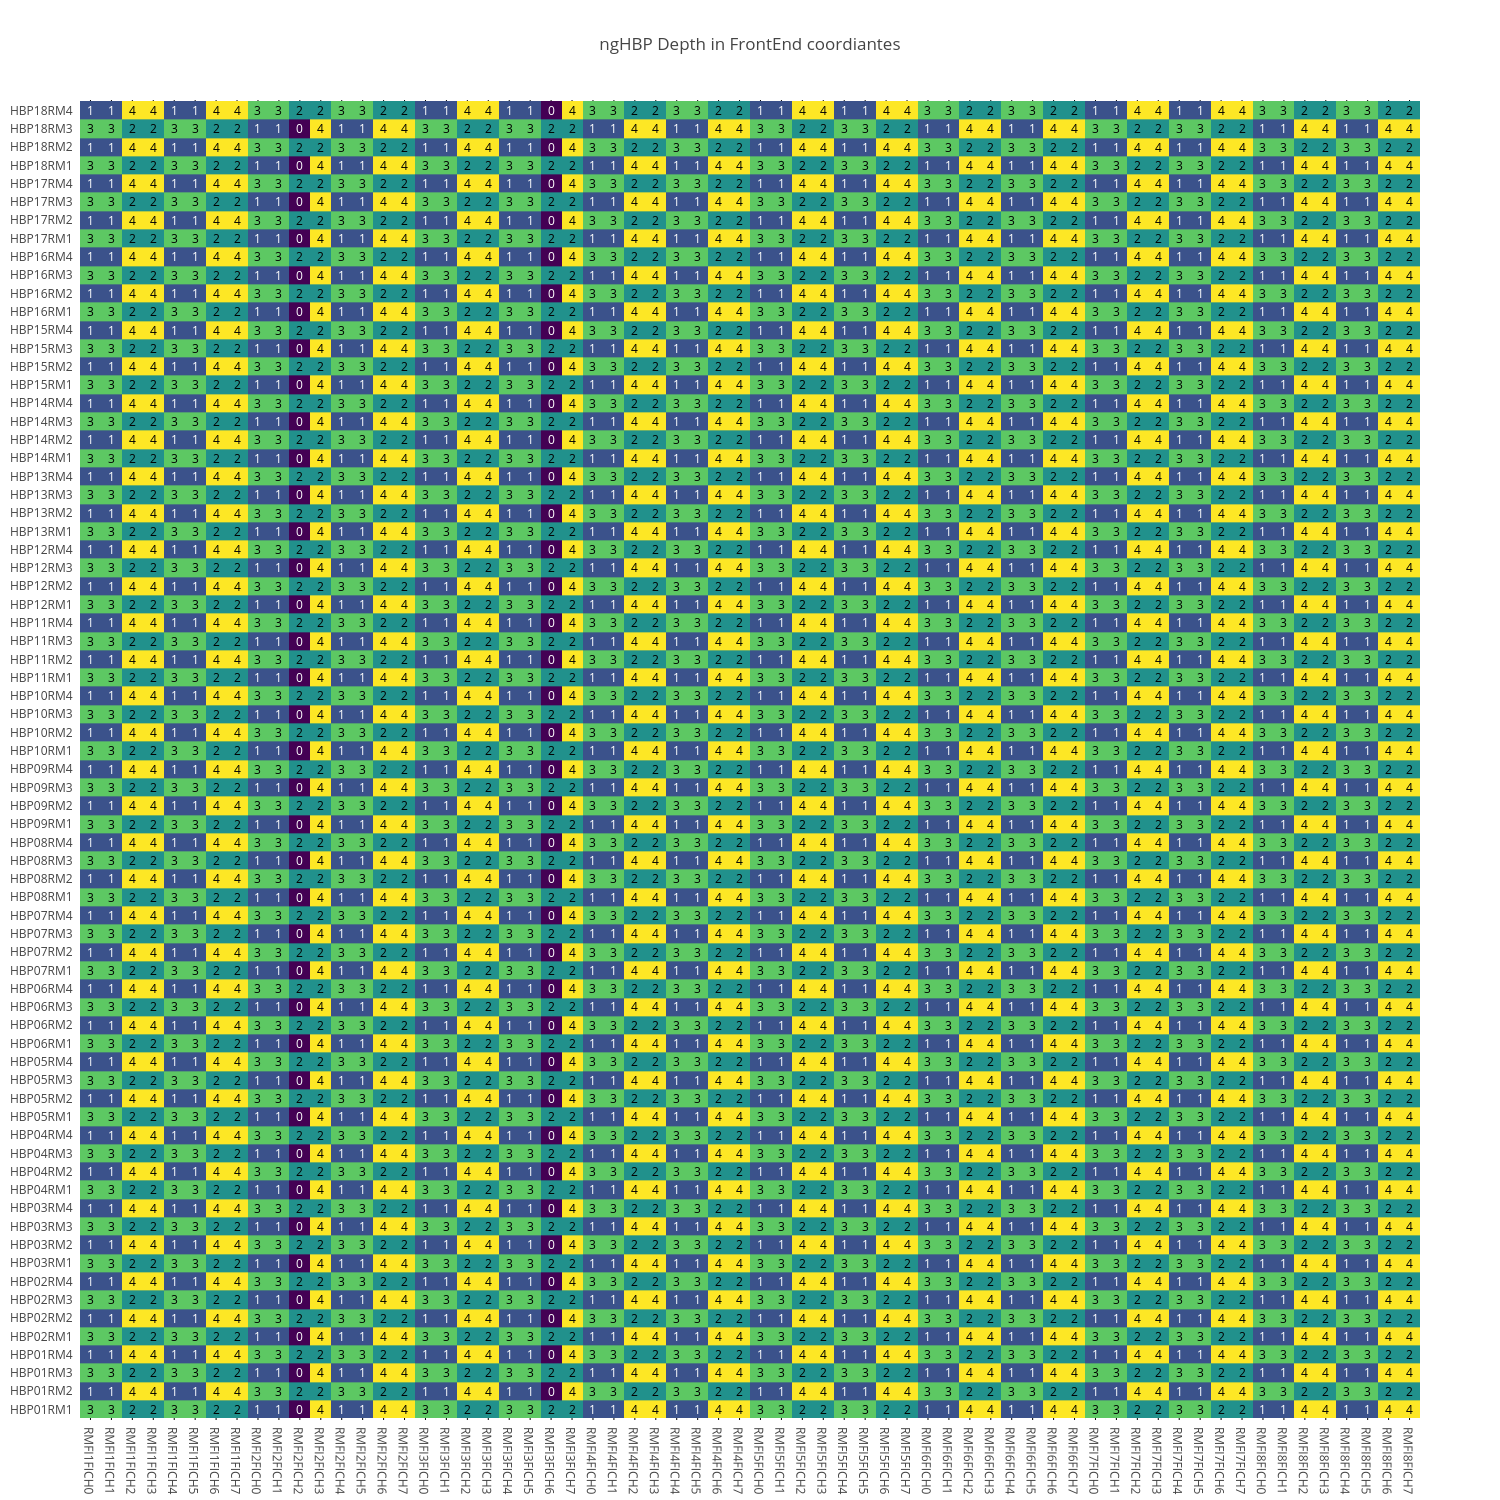
\includegraphics[angle=0,width=0.95\textwidth]{figures/appendix/ngHBP_Depth_in_FrontEnd.png}
  \end{tabular}
	\caption{HCAL (phase 2 HB, plus side) detector depth distribution in the frontend electronic coordinates.}
  \label{fig:lmapngHBPDepthFEC}
 \end{center}
\end{figure}
\clearpage

\begin{figure}[htb]
 \begin{center}
  \begin{tabular}{cc}
   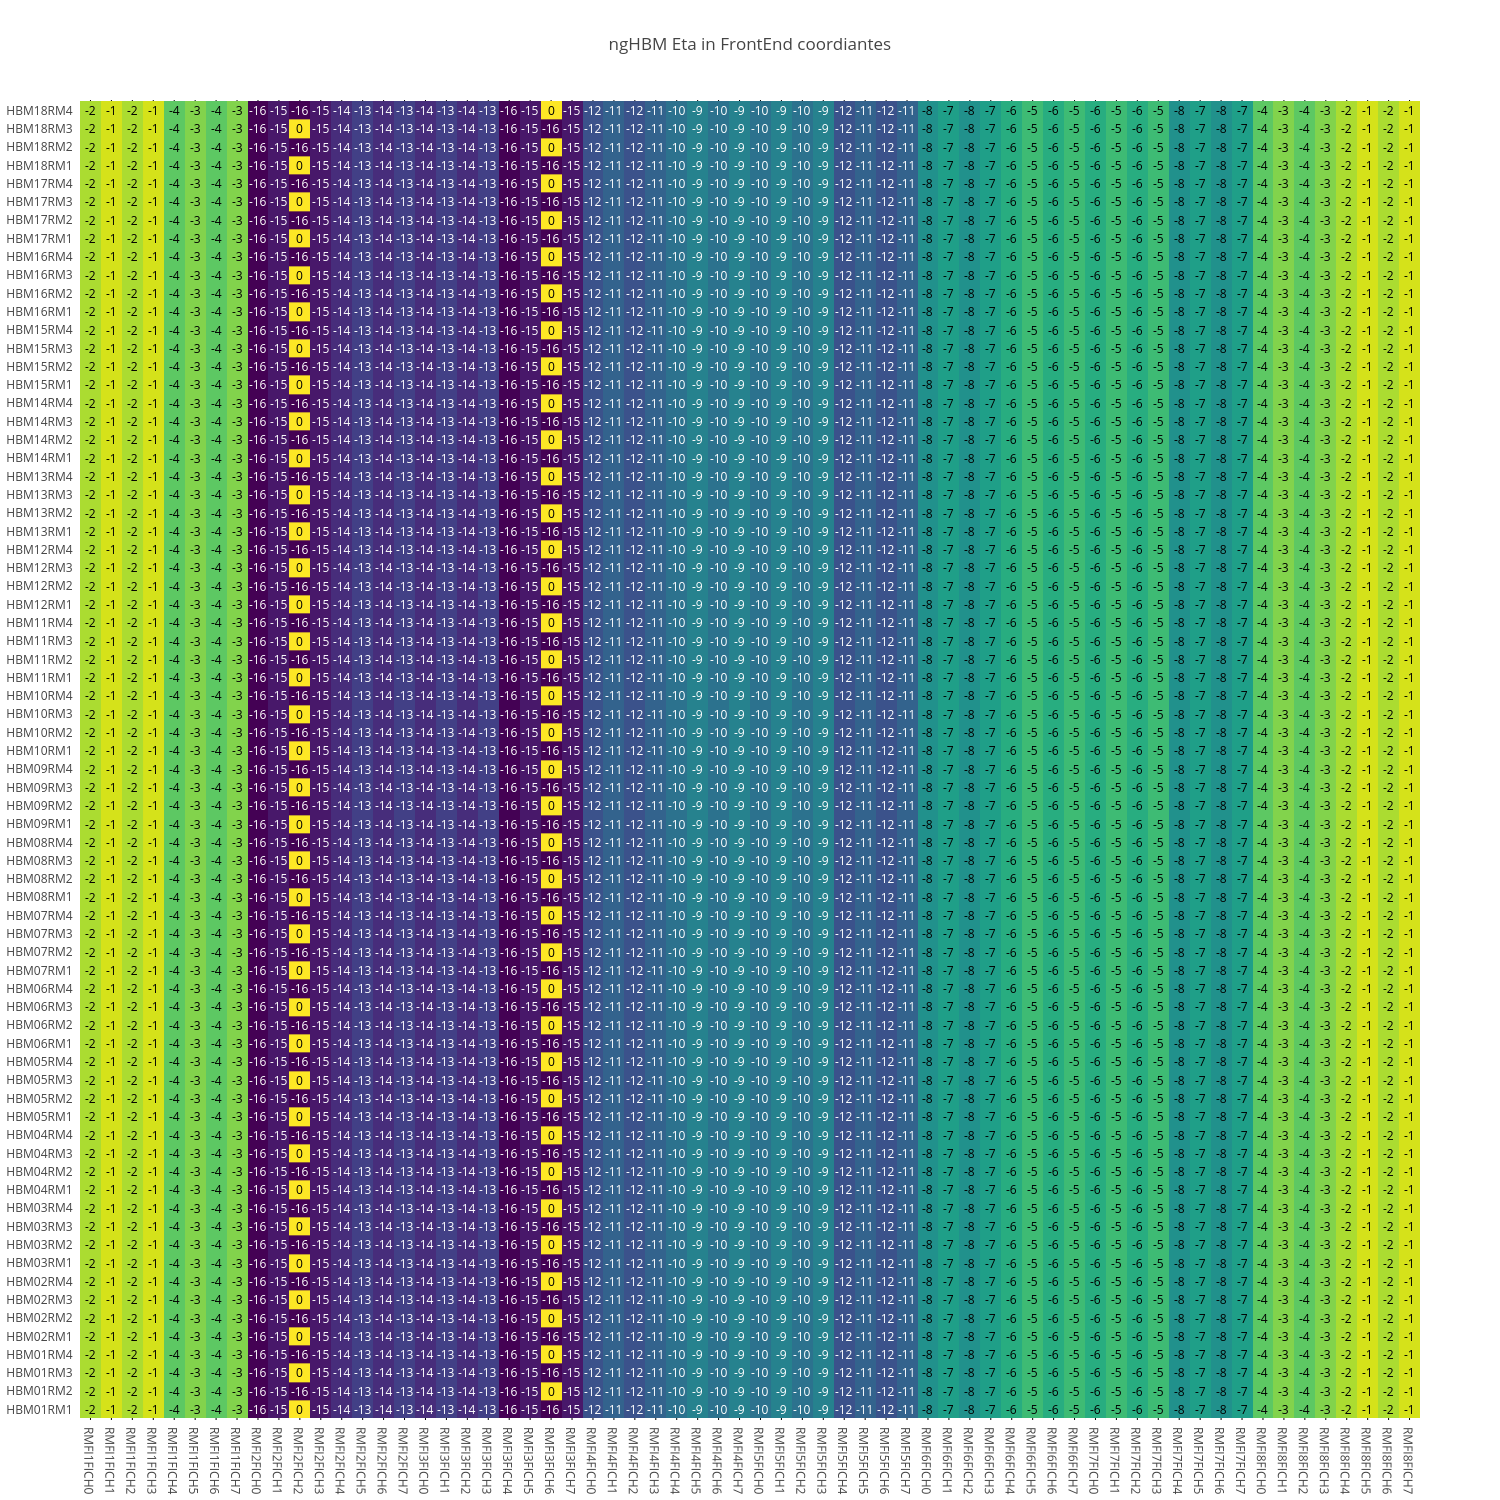
\includegraphics[angle=0,width=0.95\textwidth]{figures/appendix/ngHBM_Eta_in_FrontEnd.png}
  \end{tabular}
  \caption{HCAL (phase 2 HB, minus side) detector $\eta$ distribution in the frontend electronic coordinates.}
  \label{fig:lmapngHBMEtaFEC}
 \end{center}
\end{figure}
\clearpage

\begin{figure}[htb]
 \begin{center}
  \begin{tabular}{cc}
   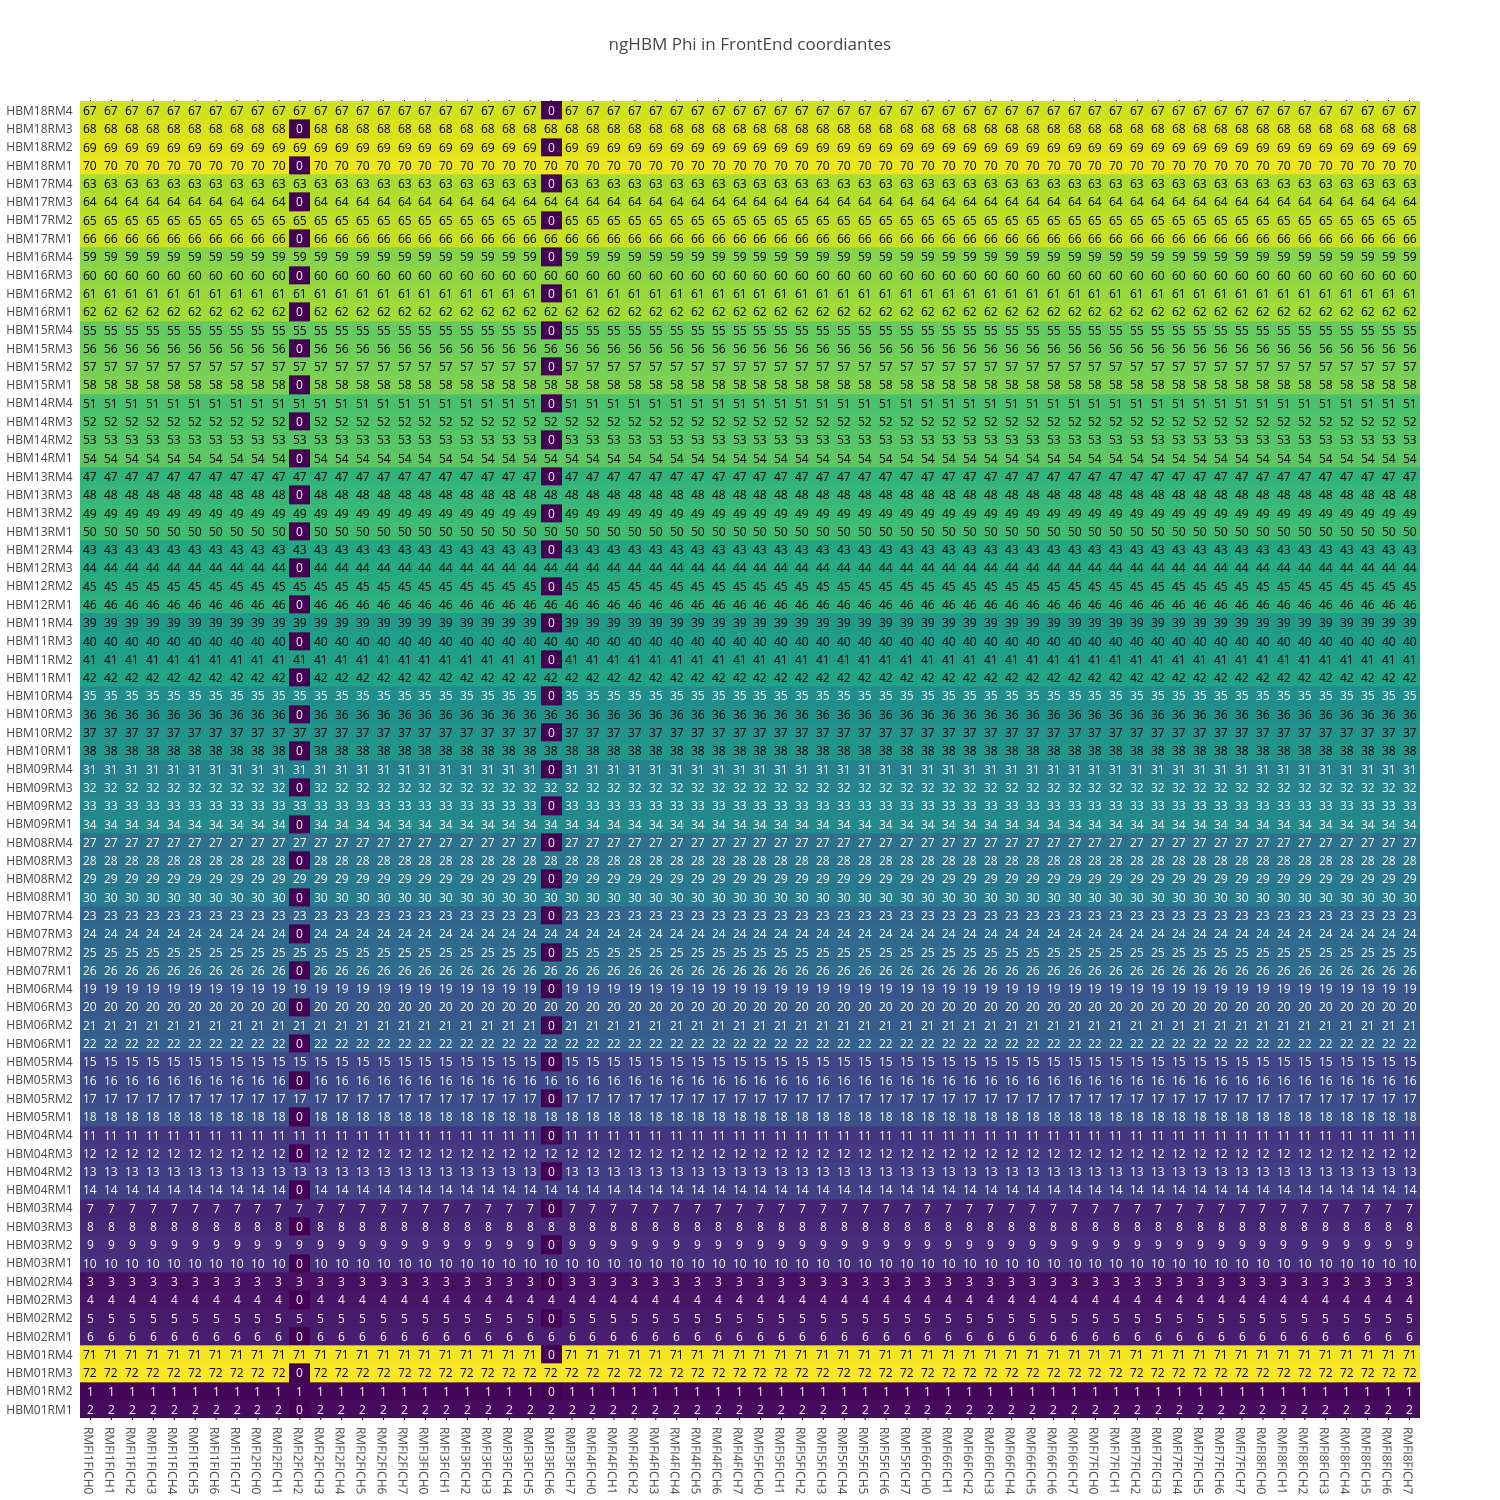
\includegraphics[angle=0,width=0.95\textwidth]{figures/appendix/ngHBM_Phi_in_FrontEnd.png}
  \end{tabular}
  \caption{HCAL (phase 2 HB, minus side) detector $\phi$ distribution in the frontend electronic coordinates.}
  \label{fig:lmapngHBMPhiFEC}
 \end{center}
\end{figure}
\clearpage

\begin{figure}[htb]
 \begin{center}
  \begin{tabular}{cc}
   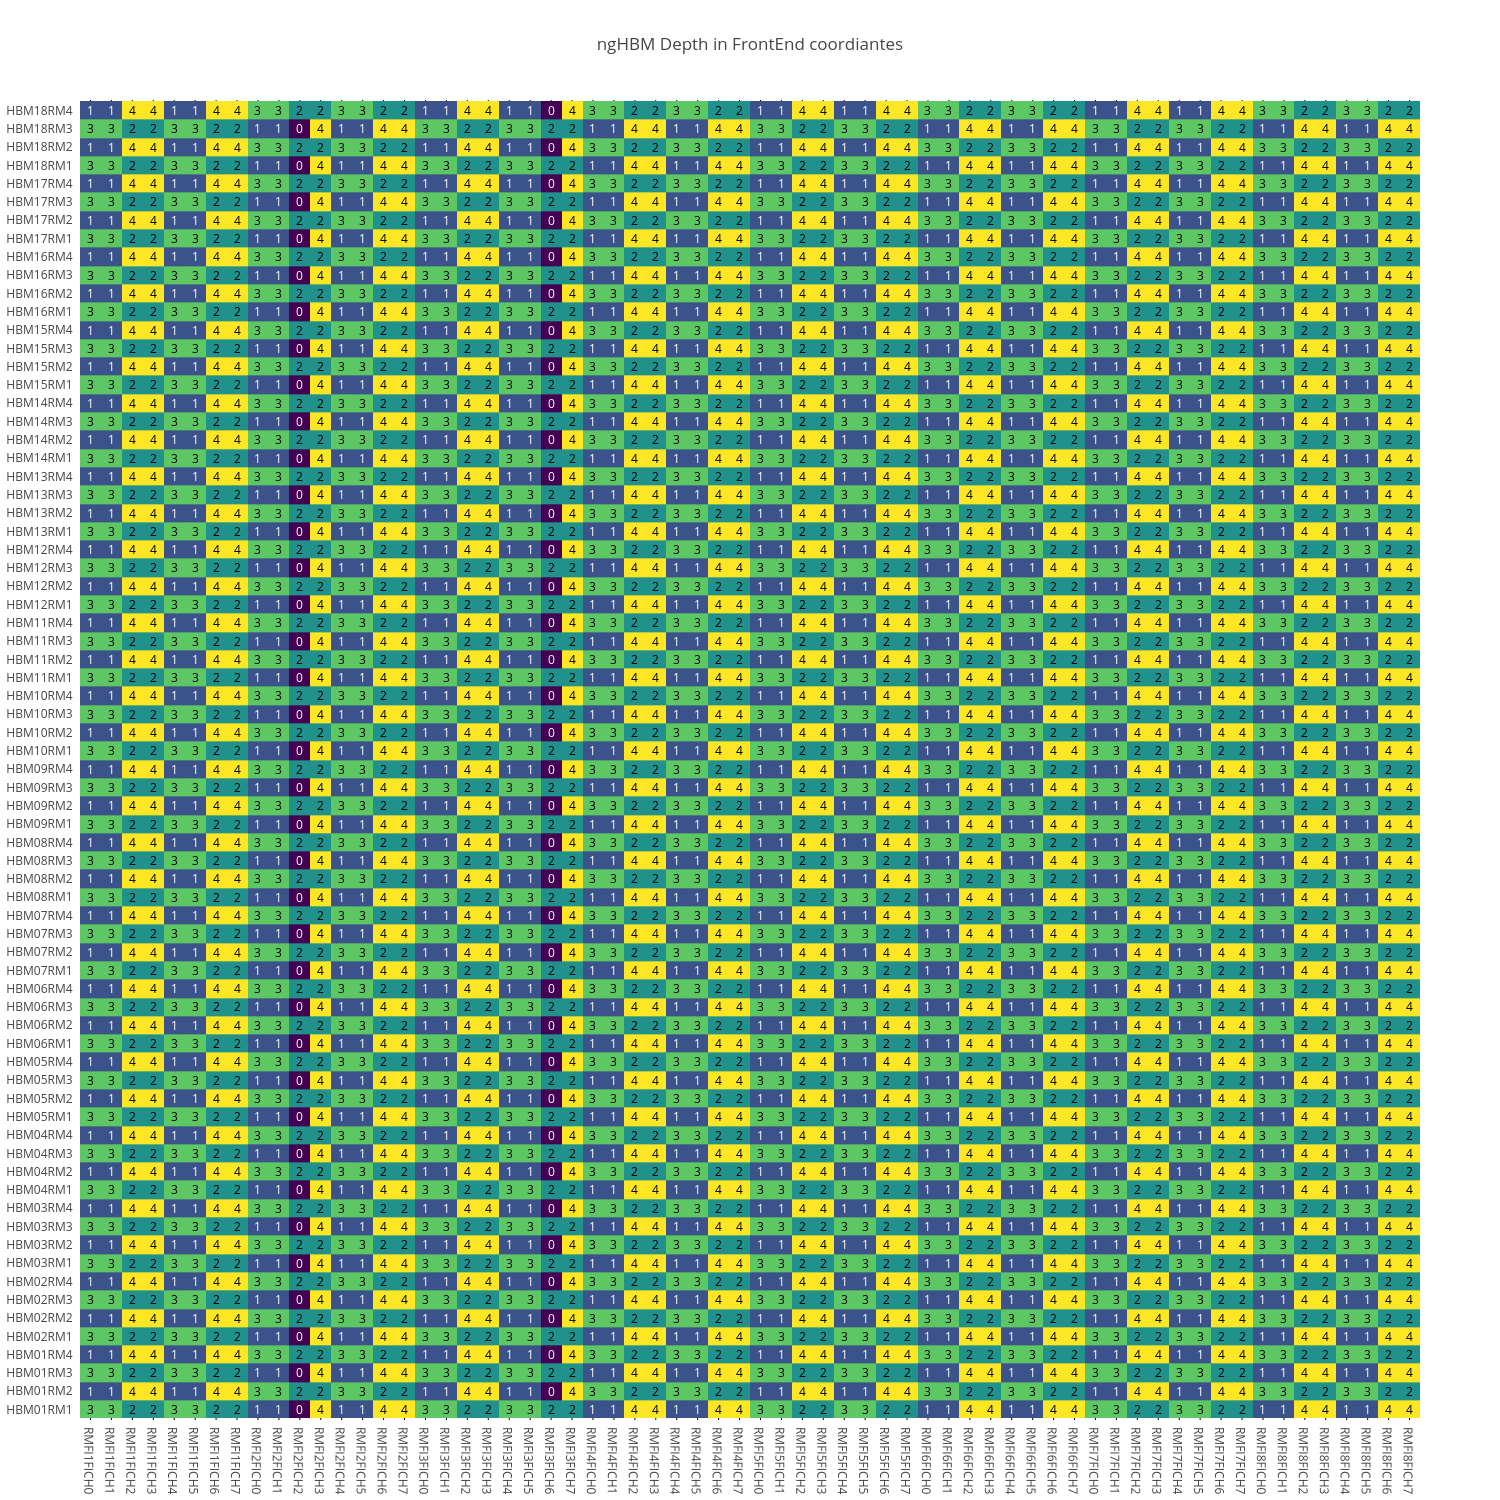
\includegraphics[angle=0,width=0.95\textwidth]{figures/appendix/ngHBM_Depth_in_FrontEnd.png}
  \end{tabular}
  \caption{HCAL (phase 2 HB, minus side) detector depth distribution in the frontend electronic coordinates.}
  \label{fig:lmapngHBMDepthFEC}
 \end{center}
\end{figure}
\clearpage

\begin{figure}[htb]
 \begin{center}
  \begin{tabular}{cc}
   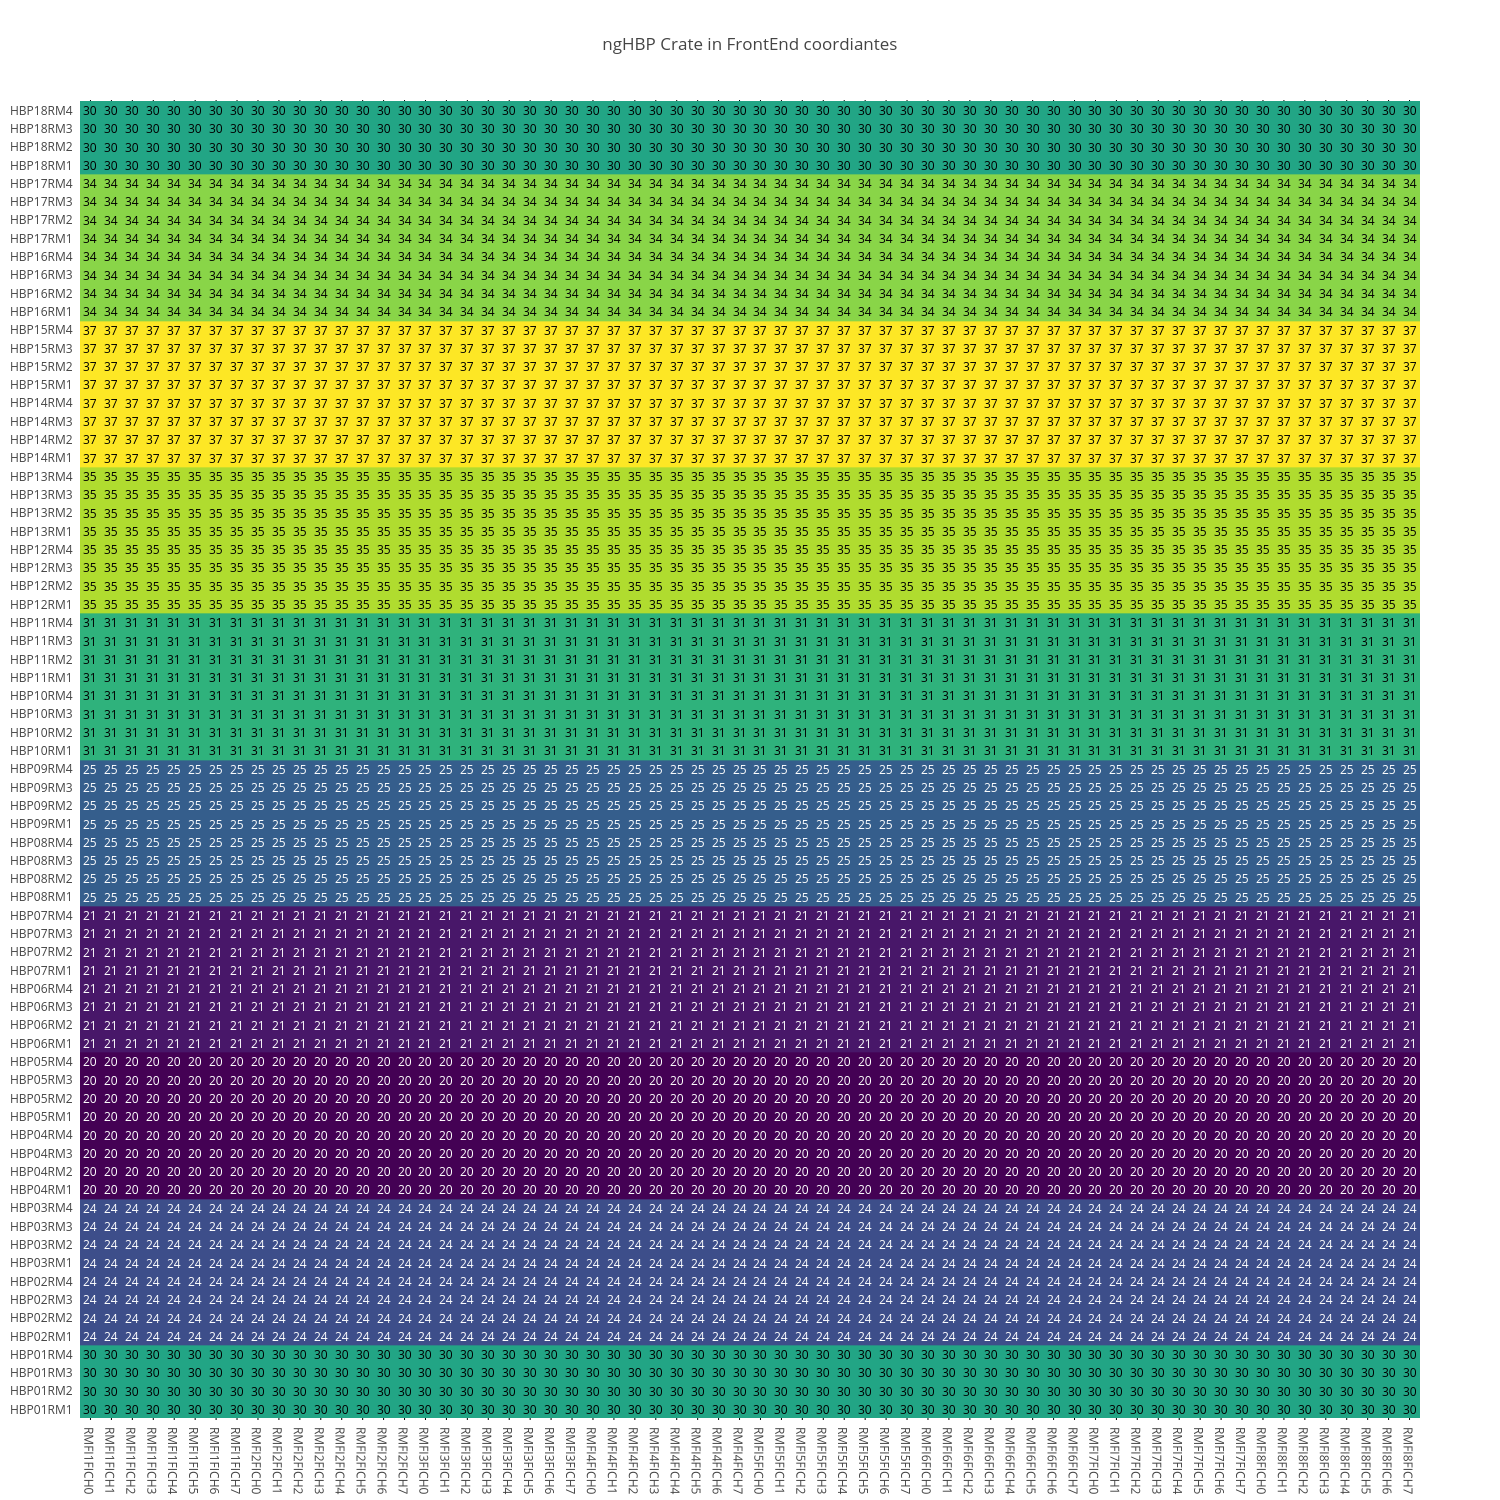
\includegraphics[angle=0,width=0.95\textwidth]{figures/appendix/ngHBP_Crate_in_FrontEnd.png}
  \end{tabular}
  \caption{HCAL (phase 2 HB, plus side) backend electronic coordinate crate distribution in the frontend electronic coordinates.}
  \label{fig:lmapngHBPCrateFEC}
 \end{center}
\end{figure}
\clearpage

\begin{figure}[htb]
 \begin{center}
  \begin{tabular}{cc}
   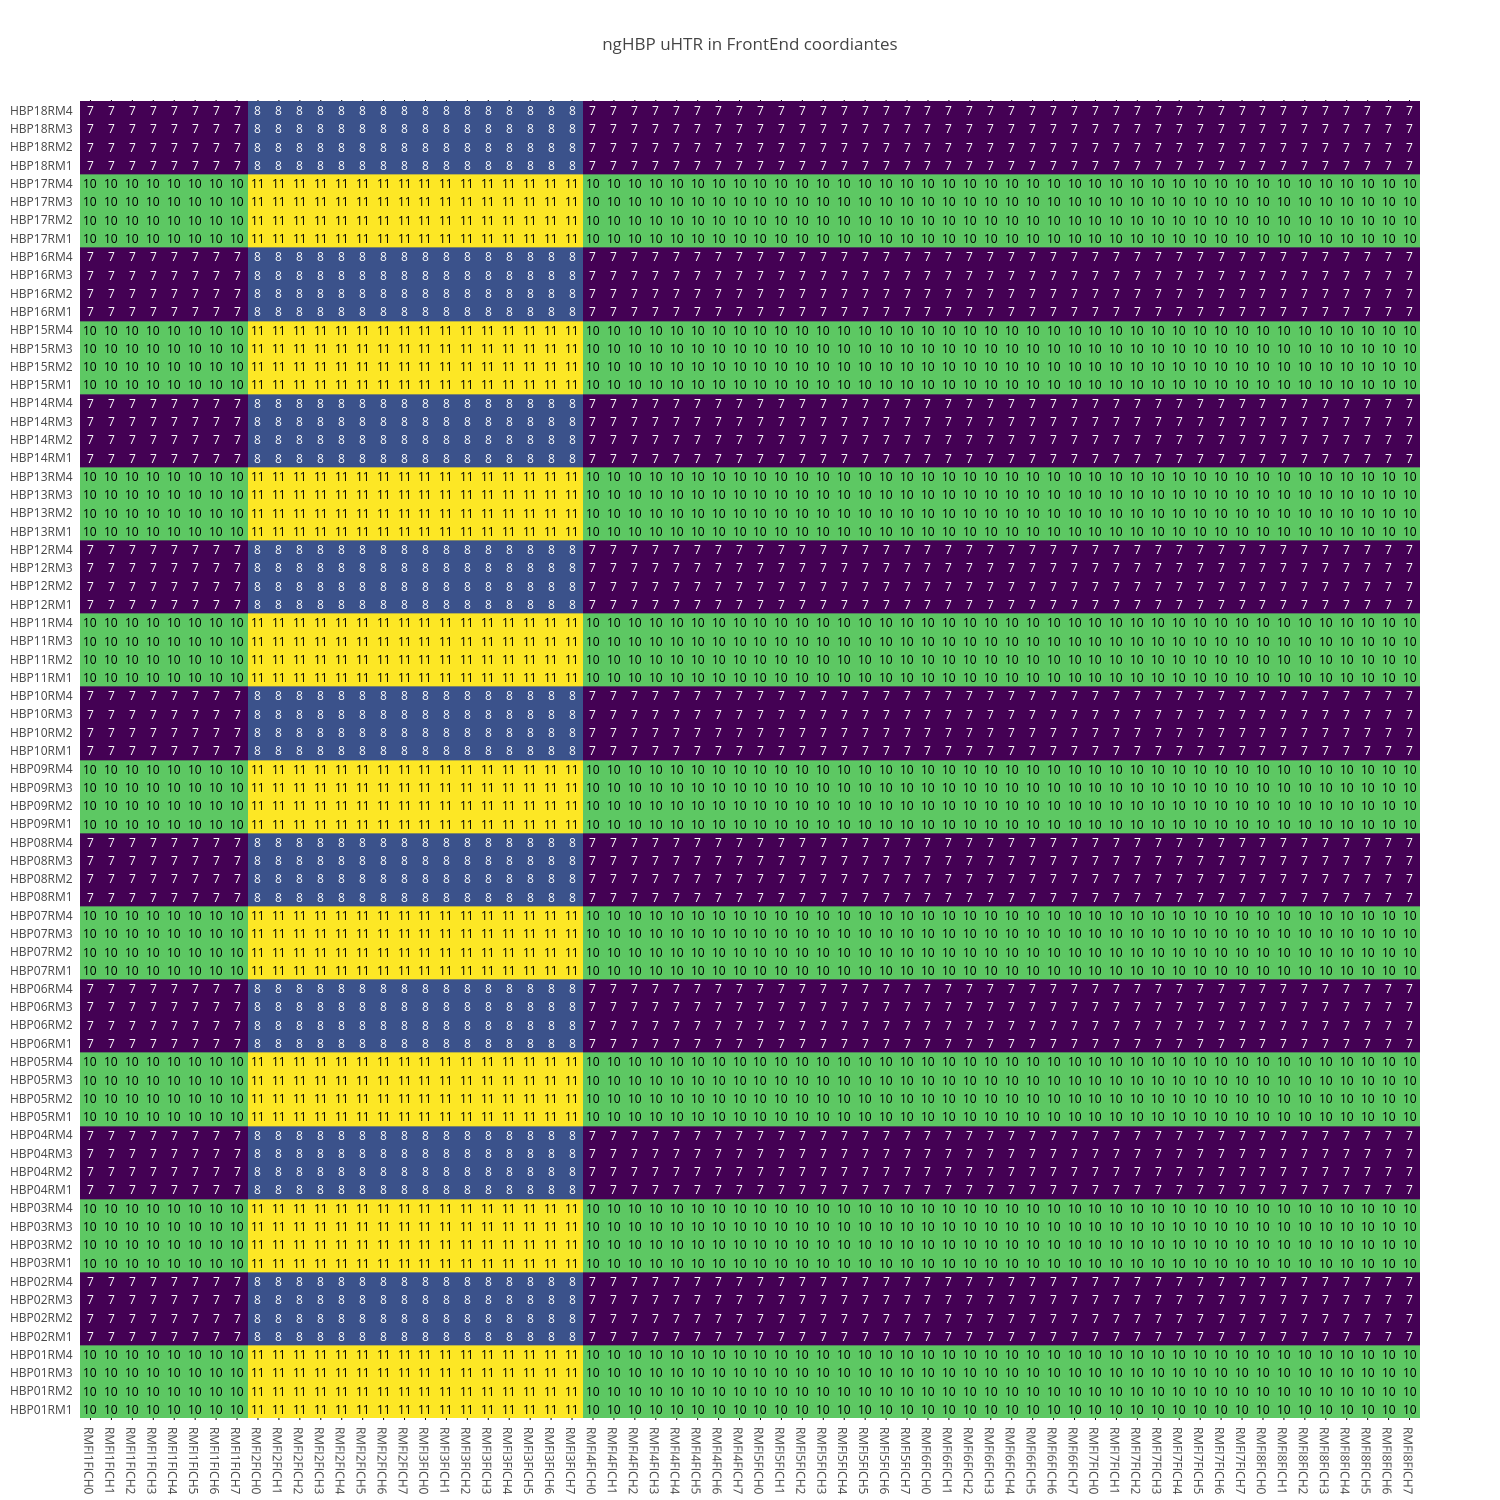
\includegraphics[angle=0,width=0.95\textwidth]{figures/appendix/ngHBP_uHTR_in_FrontEnd.png}
  \end{tabular}
  \caption{HCAL (phase 2 HB, plus side) backend electronic coordinate uHTR slot distribution in the frontend electronic coordinates.}
  \label{fig:lmapngHBPuHTRFEC}
 \end{center}
\end{figure}
\clearpage

\begin{figure}[htb]
 \begin{center}
  \begin{tabular}{cc}
   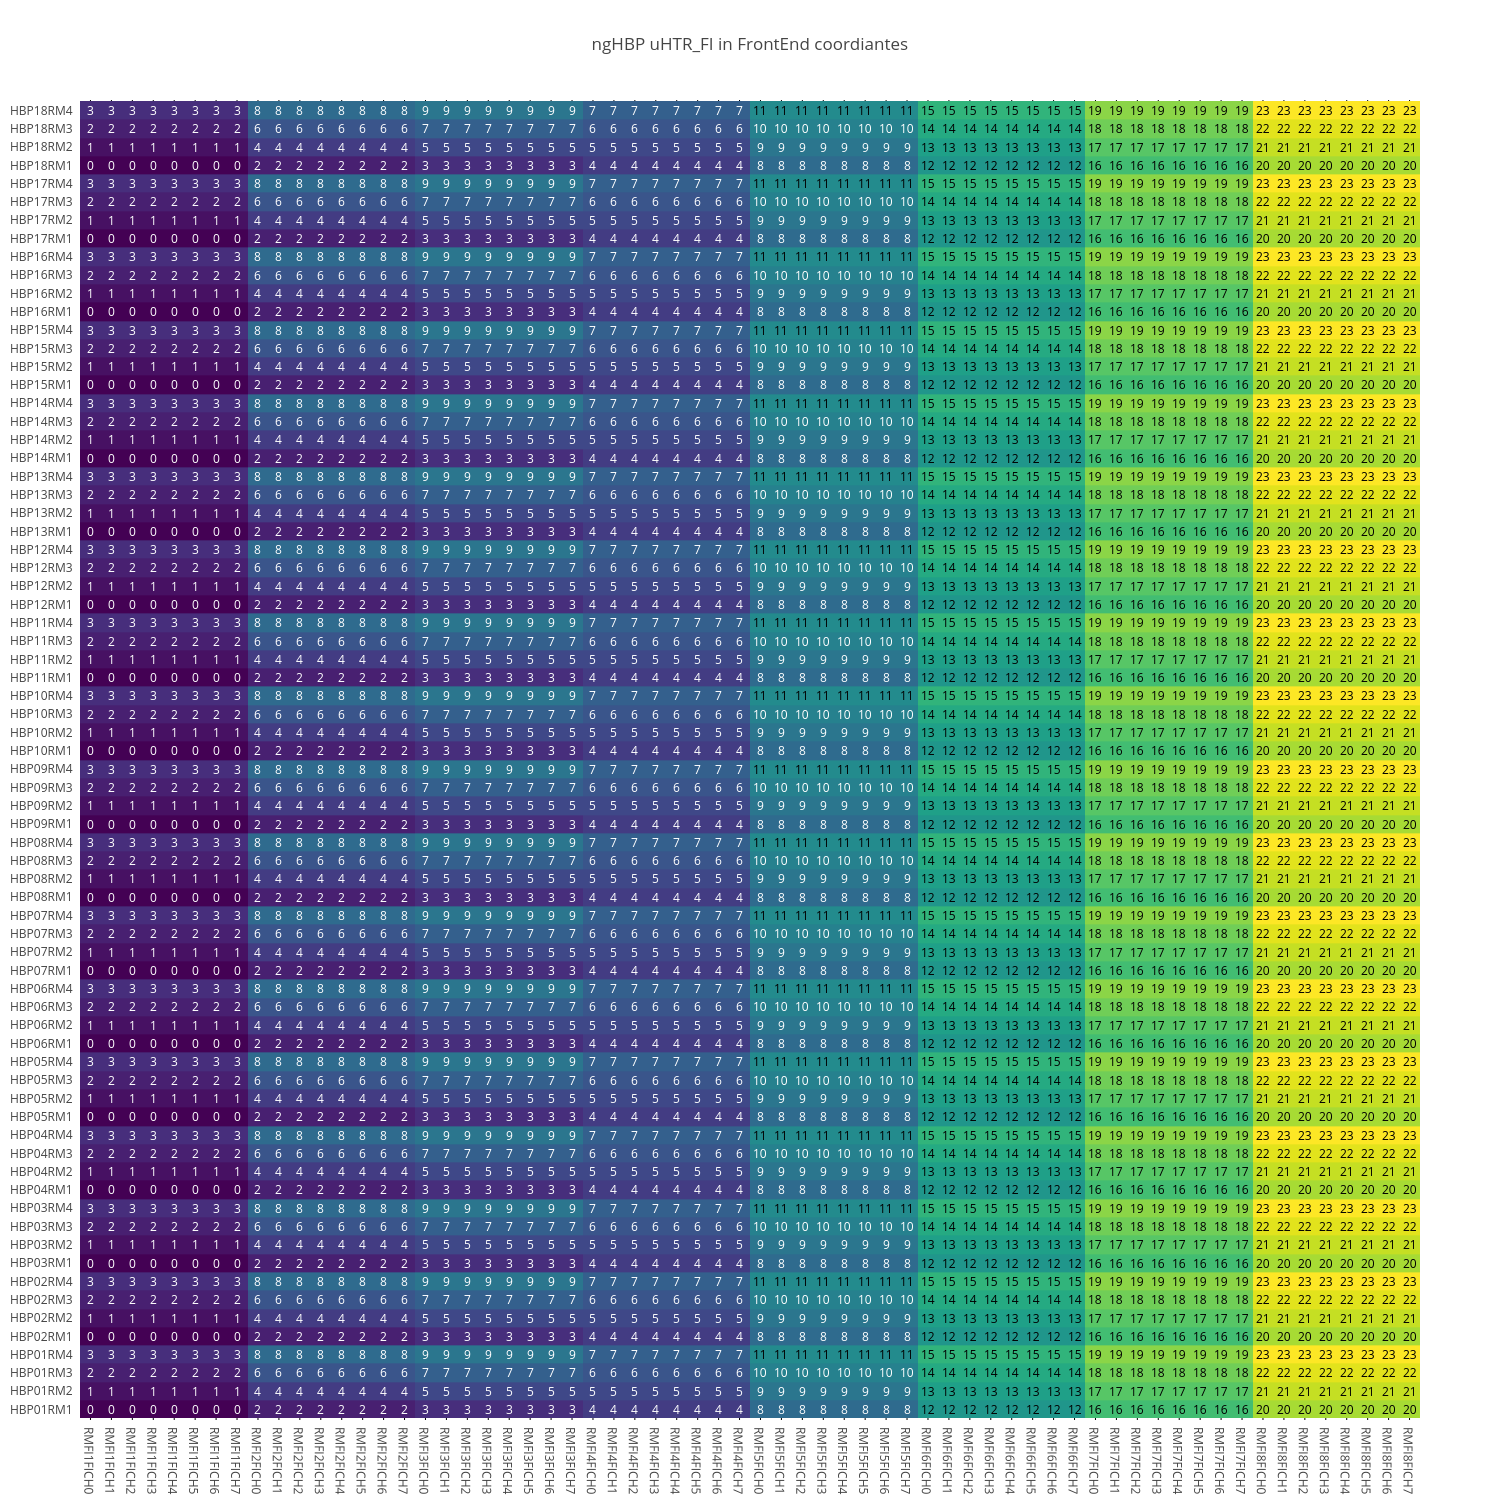
\includegraphics[angle=0,width=0.95\textwidth]{figures/appendix/ngHBP_uHTR_FI_in_FrontEnd.png}
  \end{tabular}
  \caption{HCAL (phase 2 HB, plus side) backend electronic coordinate uHTR fiber distribution in the frontend electronic coordinates.}
  \label{fig:lmapngHBPuHTRFIFEC}
 \end{center}
\end{figure}
\clearpage

\begin{figure}[htb]
 \begin{center}
  \begin{tabular}{cc}
   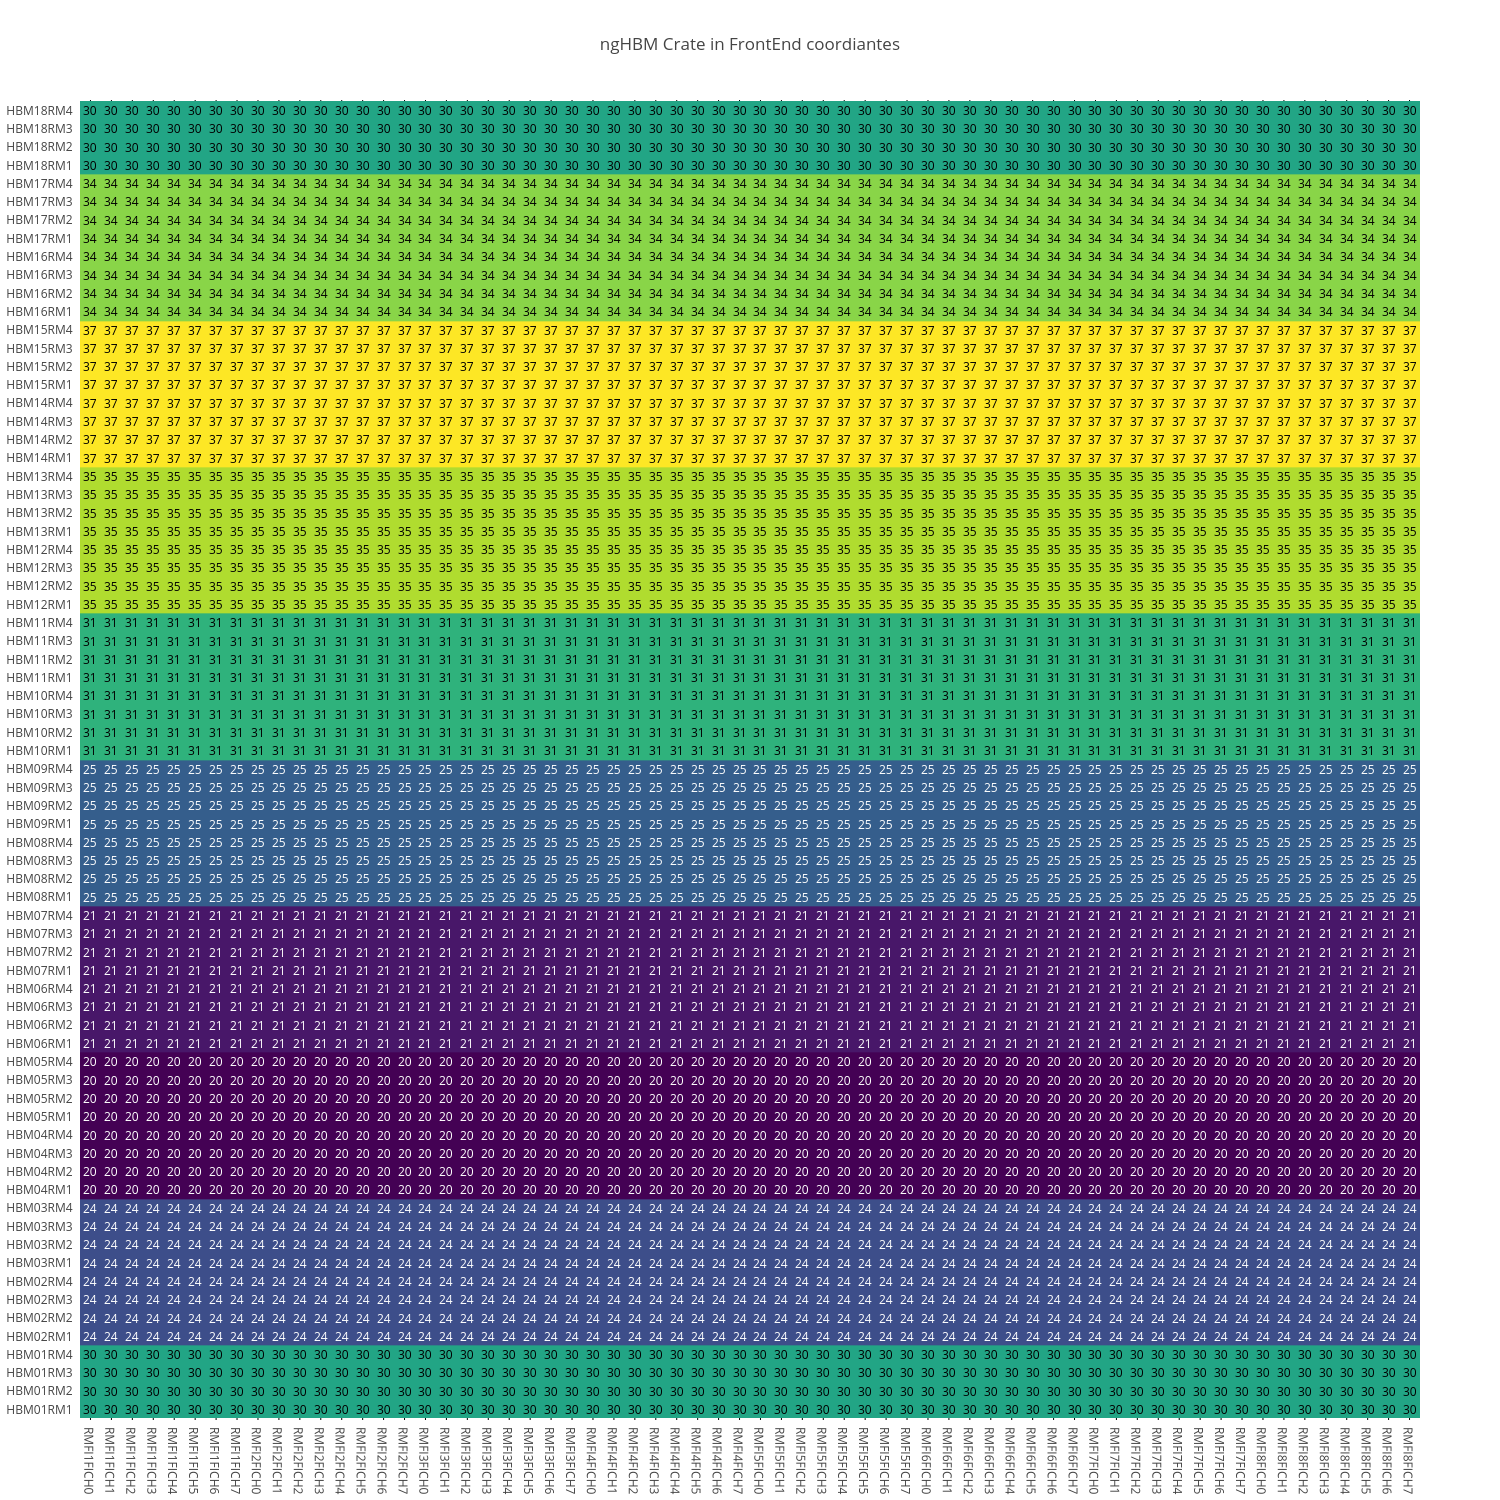
\includegraphics[angle=0,width=0.95\textwidth]{figures/appendix/ngHBM_Crate_in_FrontEnd.png}
  \end{tabular}
  \caption{HCAL (phase 2 HB, minus side) backend electronic coordinate crate distribution in the frontend electronic coordinates.}
  \label{fig:lmapngHBMCrateFEC}
 \end{center}
\end{figure}
\clearpage

\begin{figure}[htb]
 \begin{center}
  \begin{tabular}{cc}
   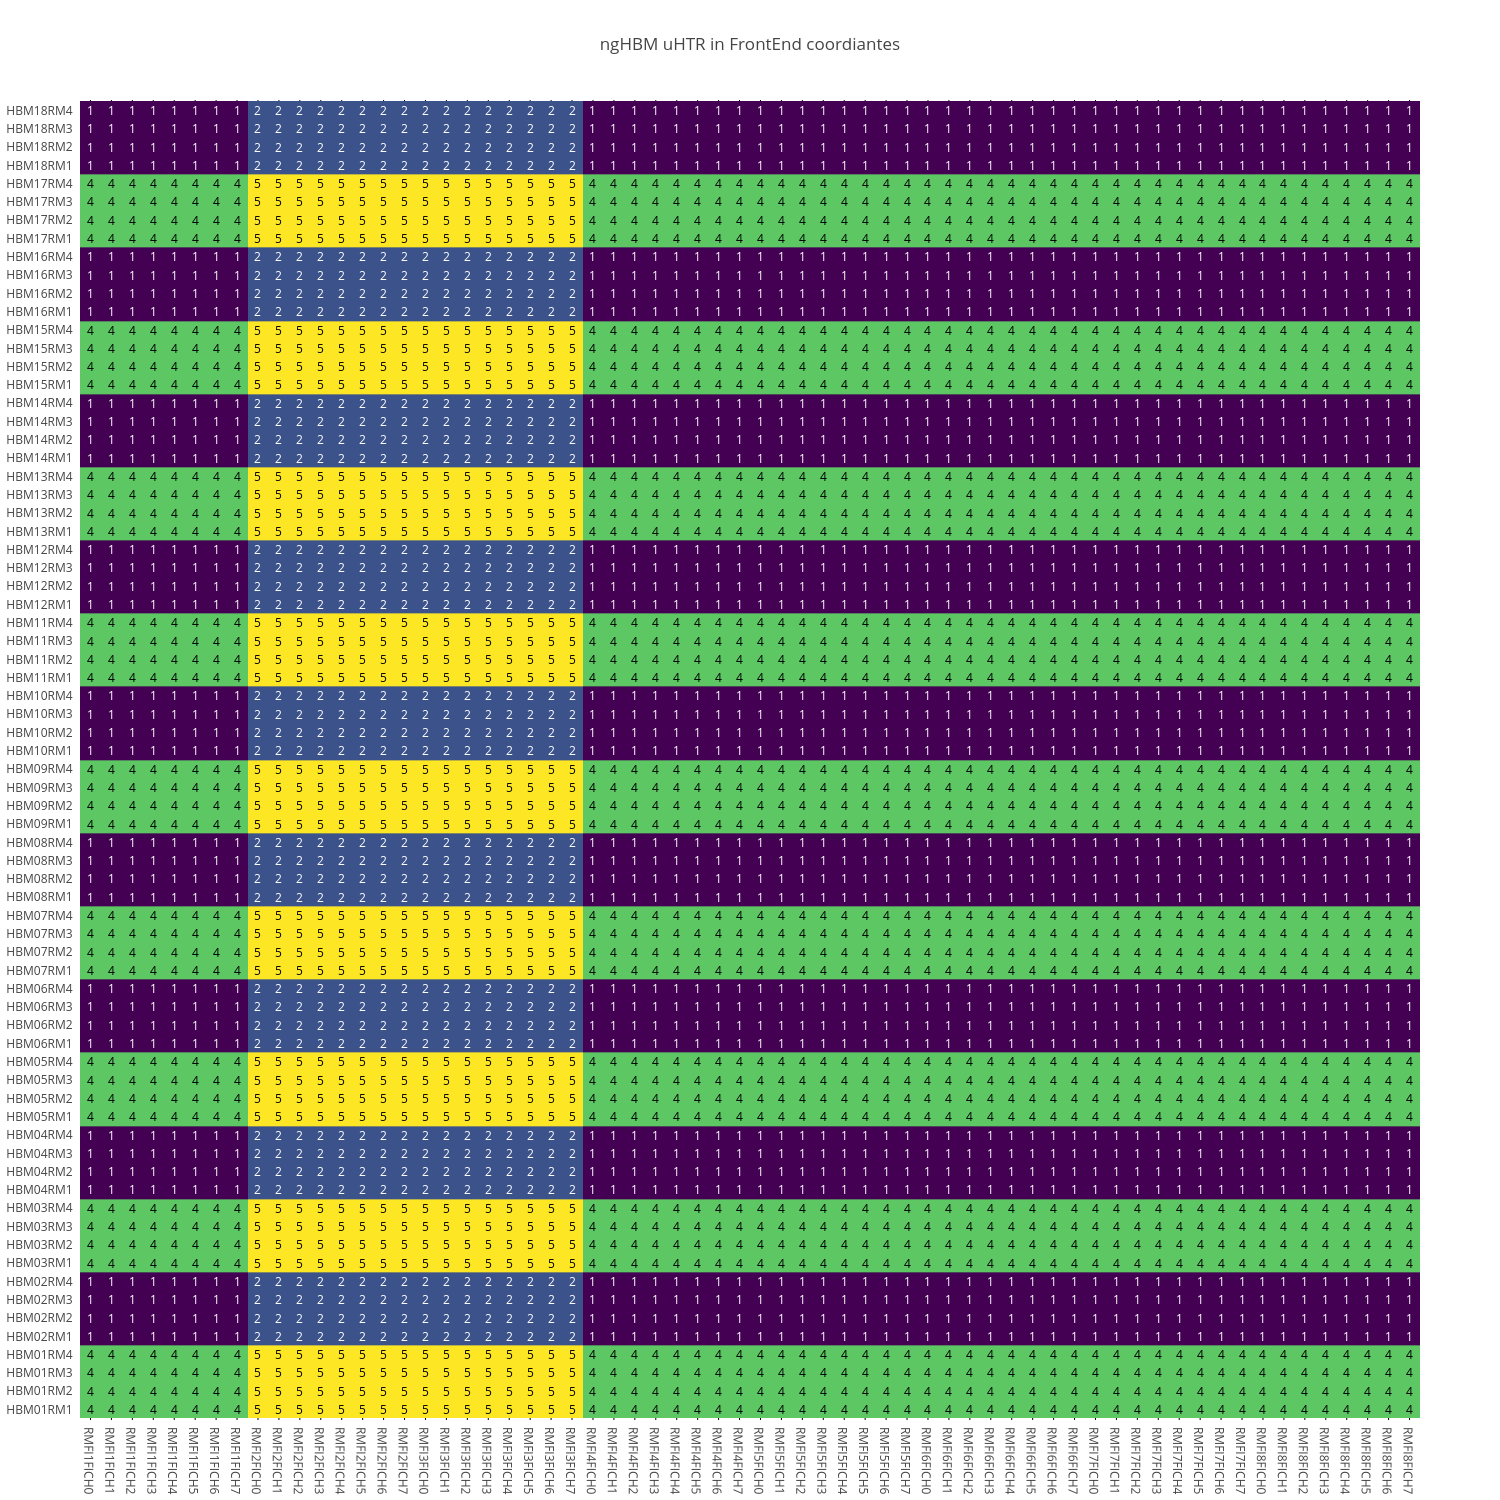
\includegraphics[angle=0,width=0.95\textwidth]{figures/appendix/ngHBM_uHTR_in_FrontEnd.png}
  \end{tabular}
  \caption{HCAL (phase 2 HB, minus side) backend electronic coordinate uHTR slot distribution in the frontend electronic coordinates.}
  \label{fig:lmapngHBMuHTRFEC}
 \end{center}
\end{figure}
\clearpage

\begin{figure}[htb]
 \begin{center}
  \begin{tabular}{cc}
   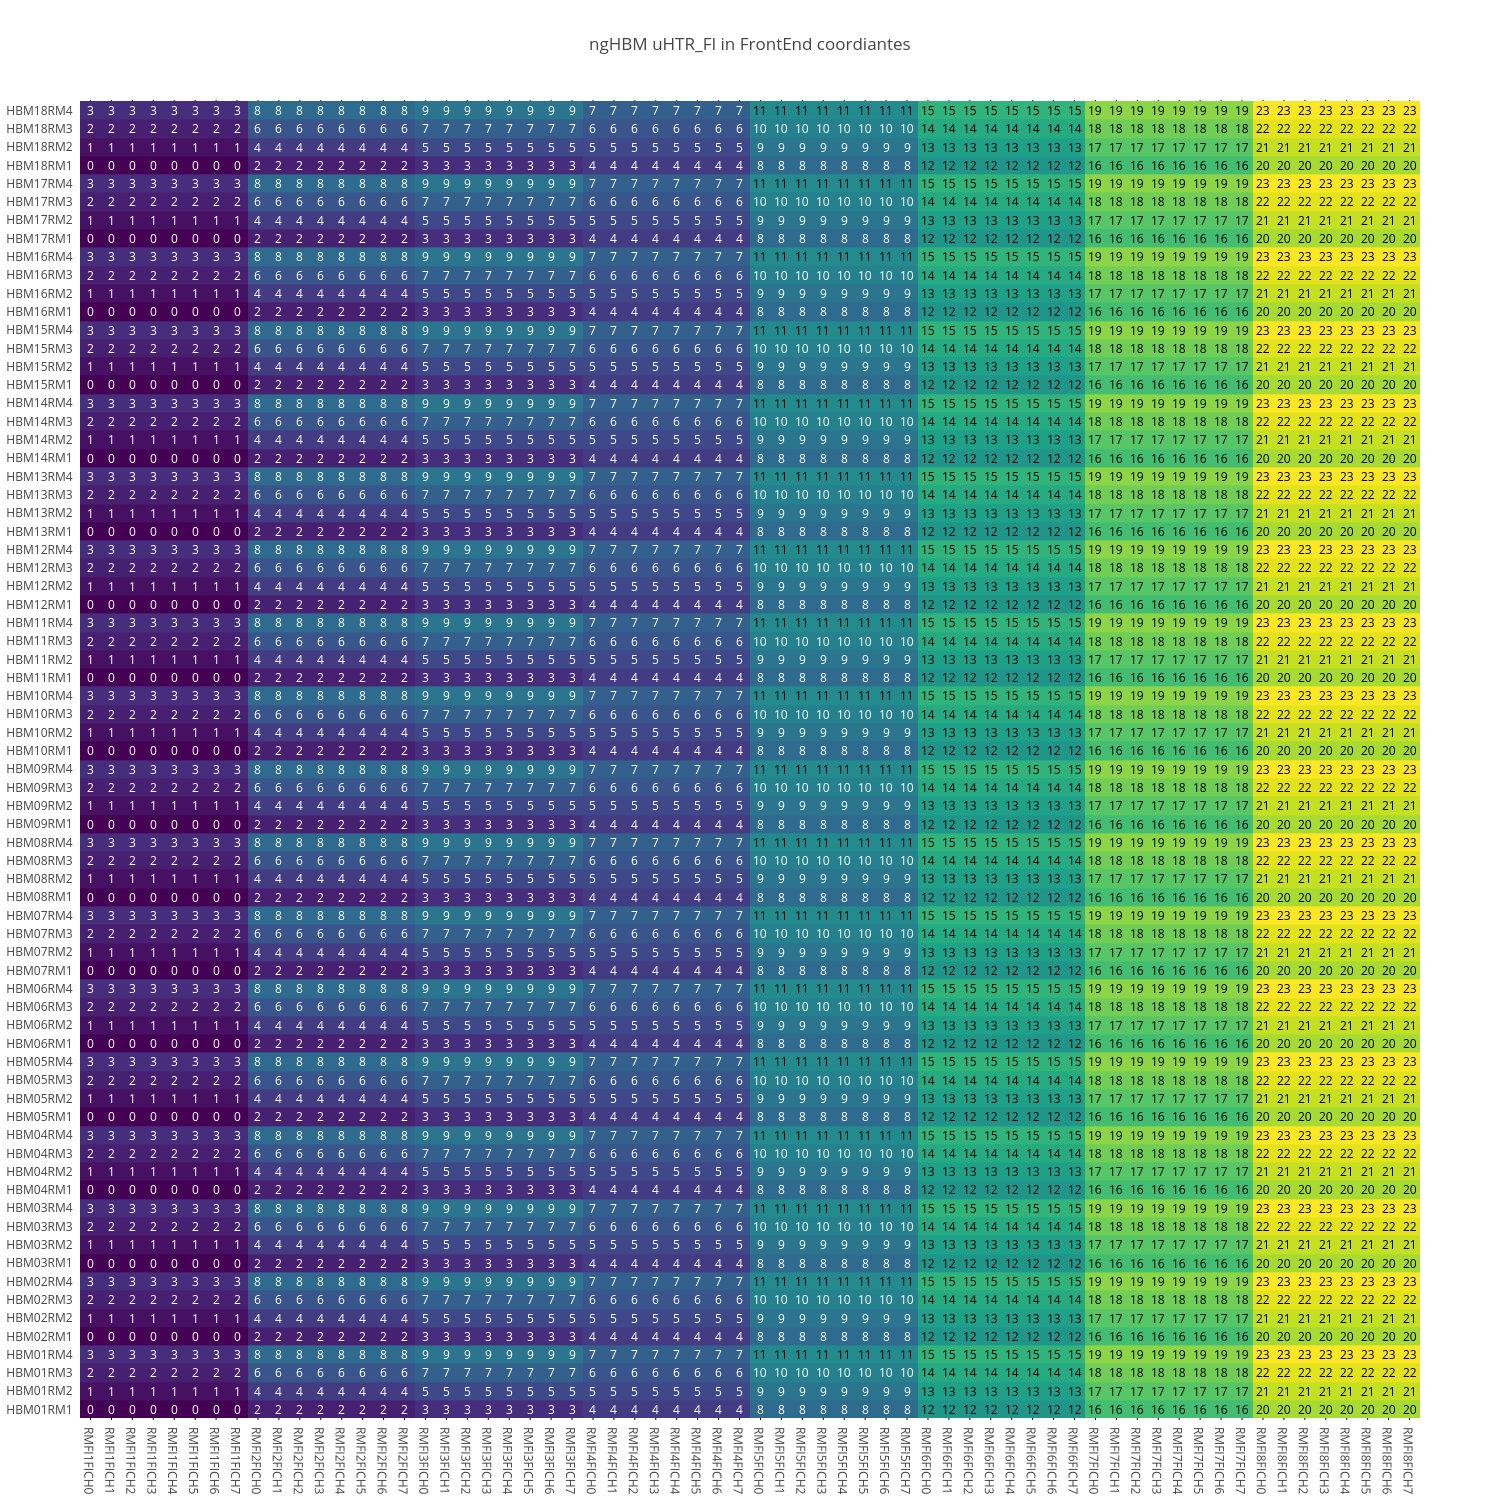
\includegraphics[angle=0,width=0.95\textwidth]{figures/appendix/ngHBM_uHTR_FI_in_FrontEnd.png}
  \end{tabular}
  \caption{HCAL (phase 2 HB, minus side) backend electronic coordinate uHTR fiber distribution in the frontend electronic coordinates.}
  \label{fig:lmapngHBMuHTRFIFEC}
 \end{center}
\end{figure}
\clearpage

\subsection{Phase 1 HE in 2018}
The 2018 HE is in SiPM+QIE11 FrontEnd+uTCA BackEnd stage. HE mapping algorithm is always more complicate than HB due to the tricky geometry structure in detector coordinates. Comparing to 2016 HE with QIE8, no swap trick inside the FrontEnd board is applied in 2018 HE. This indeed increases the difficulty for the firmware expert to pin down the latency within L1 trigger requirement. 

The phase 1 2018 HE validation plots are shown from Fig~\ref{fig:lmapngHEPEtaFEC} to Fig~\ref{fig:lmapngHEMuHTRFIFEC}. There are 6912 readout channels in phase 1 HE. 6768 channels are physical readout channel, corresponding to actual tower and layer on detector. 144 of them are dummy calibration channels, which are readout by FrontEnd with no corresponding detector components. Those dummy calibration channels are labeled as “HEX” channels. HEX channels are distributed among 144 HE readout modules, on four different locations: RM fiber 2 fiber channel 1, RM fiber 3 fiber channel 6, RM fiber 5 fiber channel 5 and RM fiber 7 fiber channel 1. BackEnd electronics are still in 12 uHTR and 24 uHTR fibers, but number of fiber channels per fiber is increased from 3 to 6, to accommodating more readout channels, comparing with 2016 HE.
\clearpage

\begin{figure}[htb]
 \begin{center}
  \begin{tabular}{cc}
   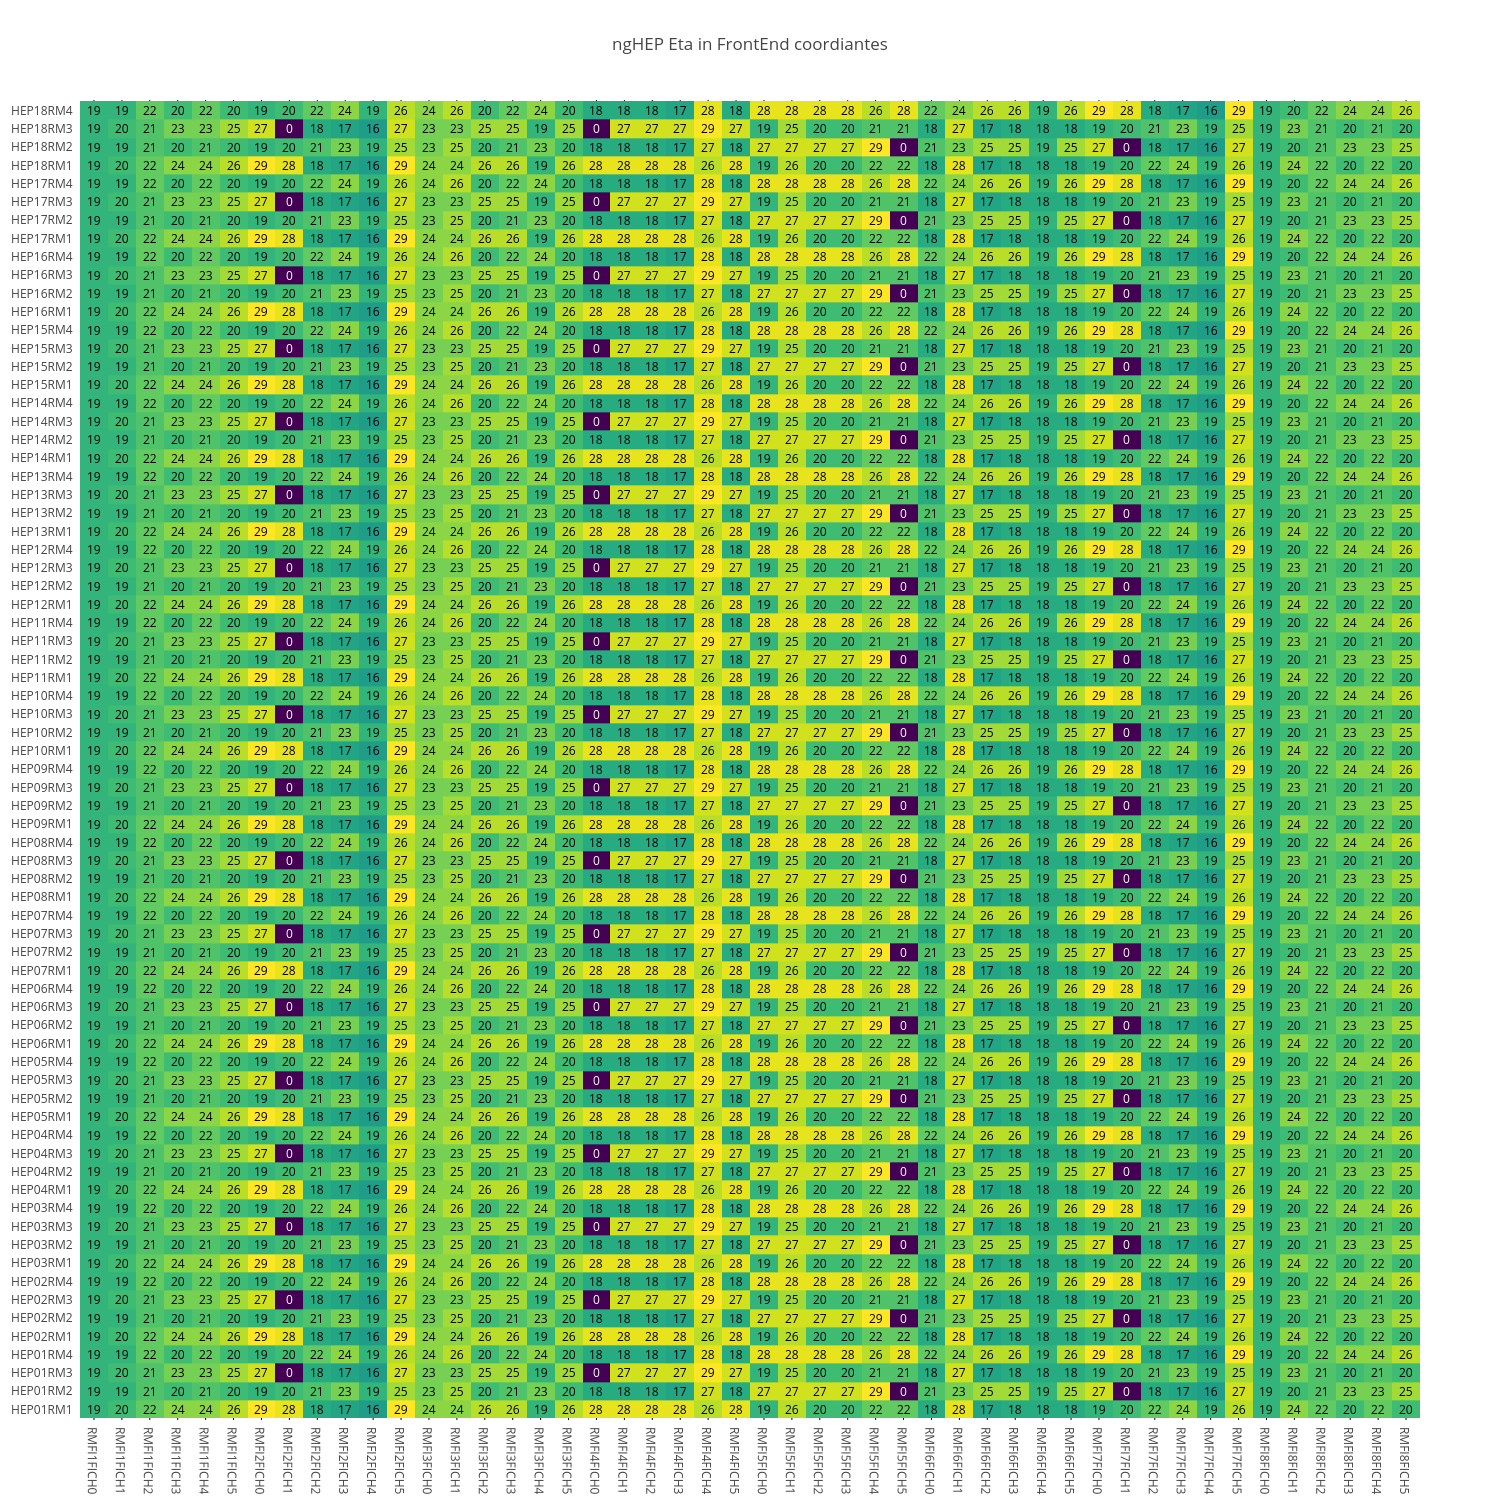
\includegraphics[angle=0,width=0.95\textwidth]{figures/appendix/ngHEP_Eta_in_FrontEnd.png}
  \end{tabular}
	\caption{HCAL (phase 1 HE, plus side) detector $\eta$ distribution in the frontend electronic coordinates.}
  \label{fig:lmapngHEPEtaFEC}
 \end{center}
\end{figure}
\clearpage

\begin{figure}[htb]
 \begin{center}
  \begin{tabular}{cc}
   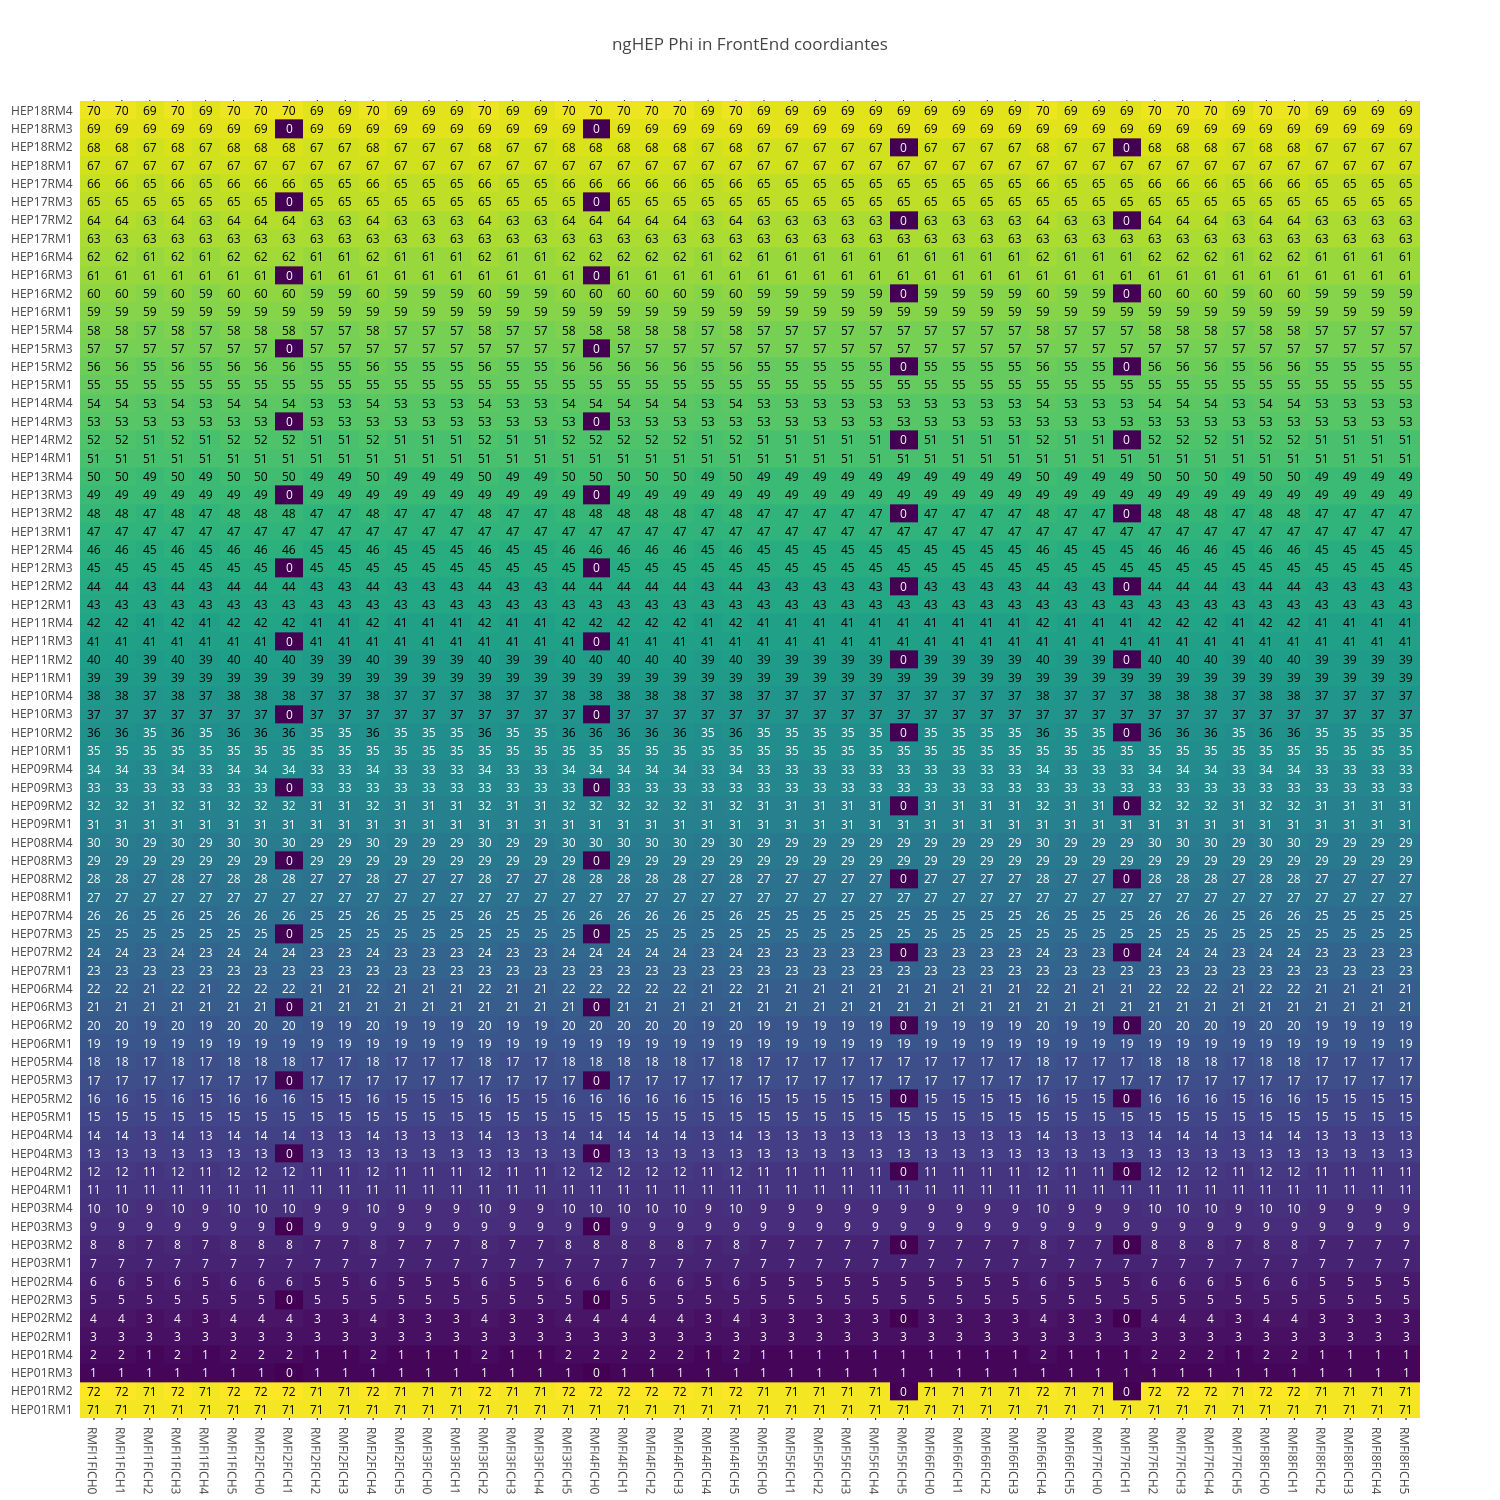
\includegraphics[angle=0,width=0.95\textwidth]{figures/appendix/ngHEP_Phi_in_FrontEnd.png}
  \end{tabular}
	\caption{HCAL (phase 1 HE, plus side) detector $\phi$ distribution in the frontend electronic coordinates.}
  \label{fig:lmapngHEPPhiFEC}
 \end{center}
\end{figure}
\clearpage

\begin{figure}[htb]
 \begin{center}
  \begin{tabular}{cc}
   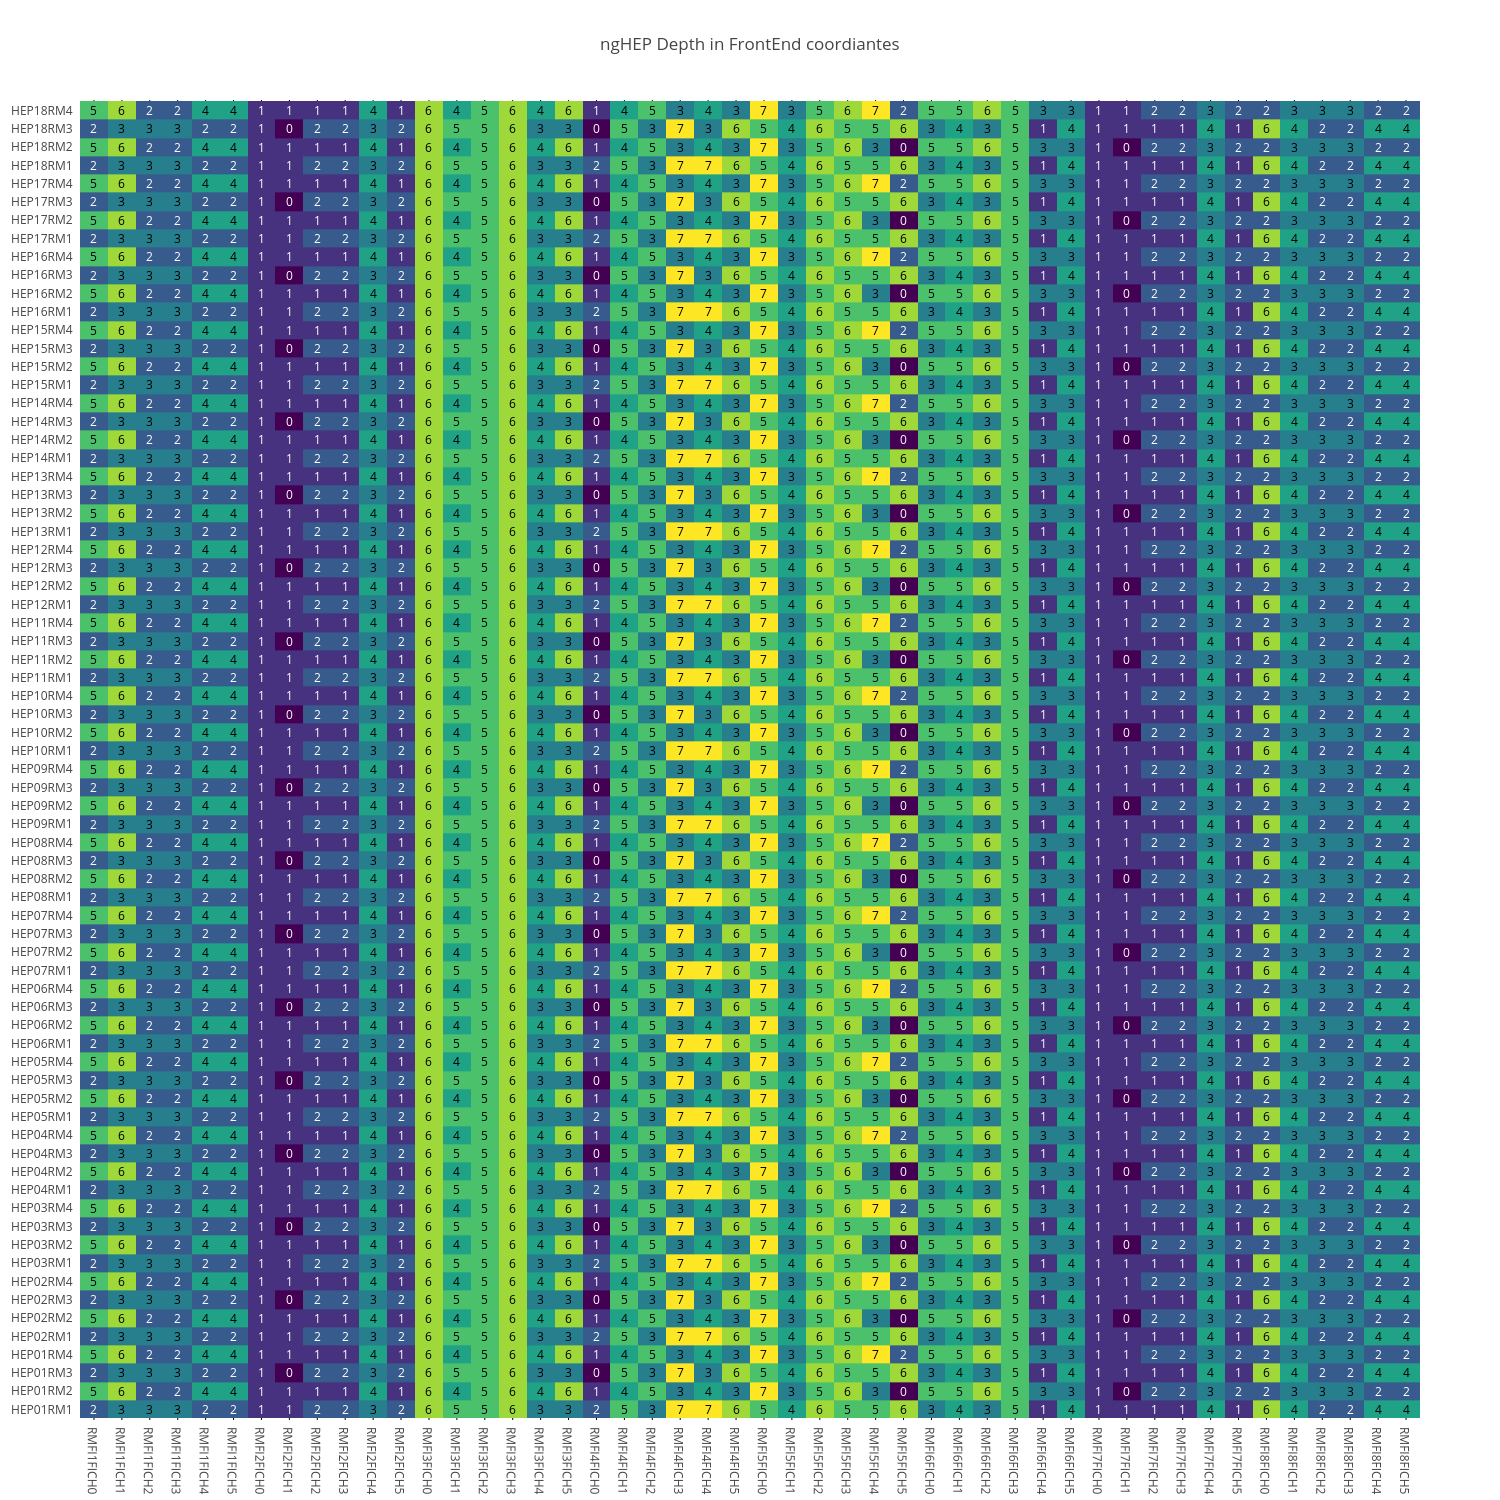
\includegraphics[angle=0,width=0.95\textwidth]{figures/appendix/ngHEP_Depth_in_FrontEnd.png}
  \end{tabular}
	\caption{HCAL (phase 1 HE, plus side) detector depth distribution in the frontend electronic coordinates.}
  \label{fig:lmapngHEPDepthFEC}
 \end{center}
\end{figure}
\clearpage

\begin{figure}[htb]
 \begin{center}
  \begin{tabular}{cc}
   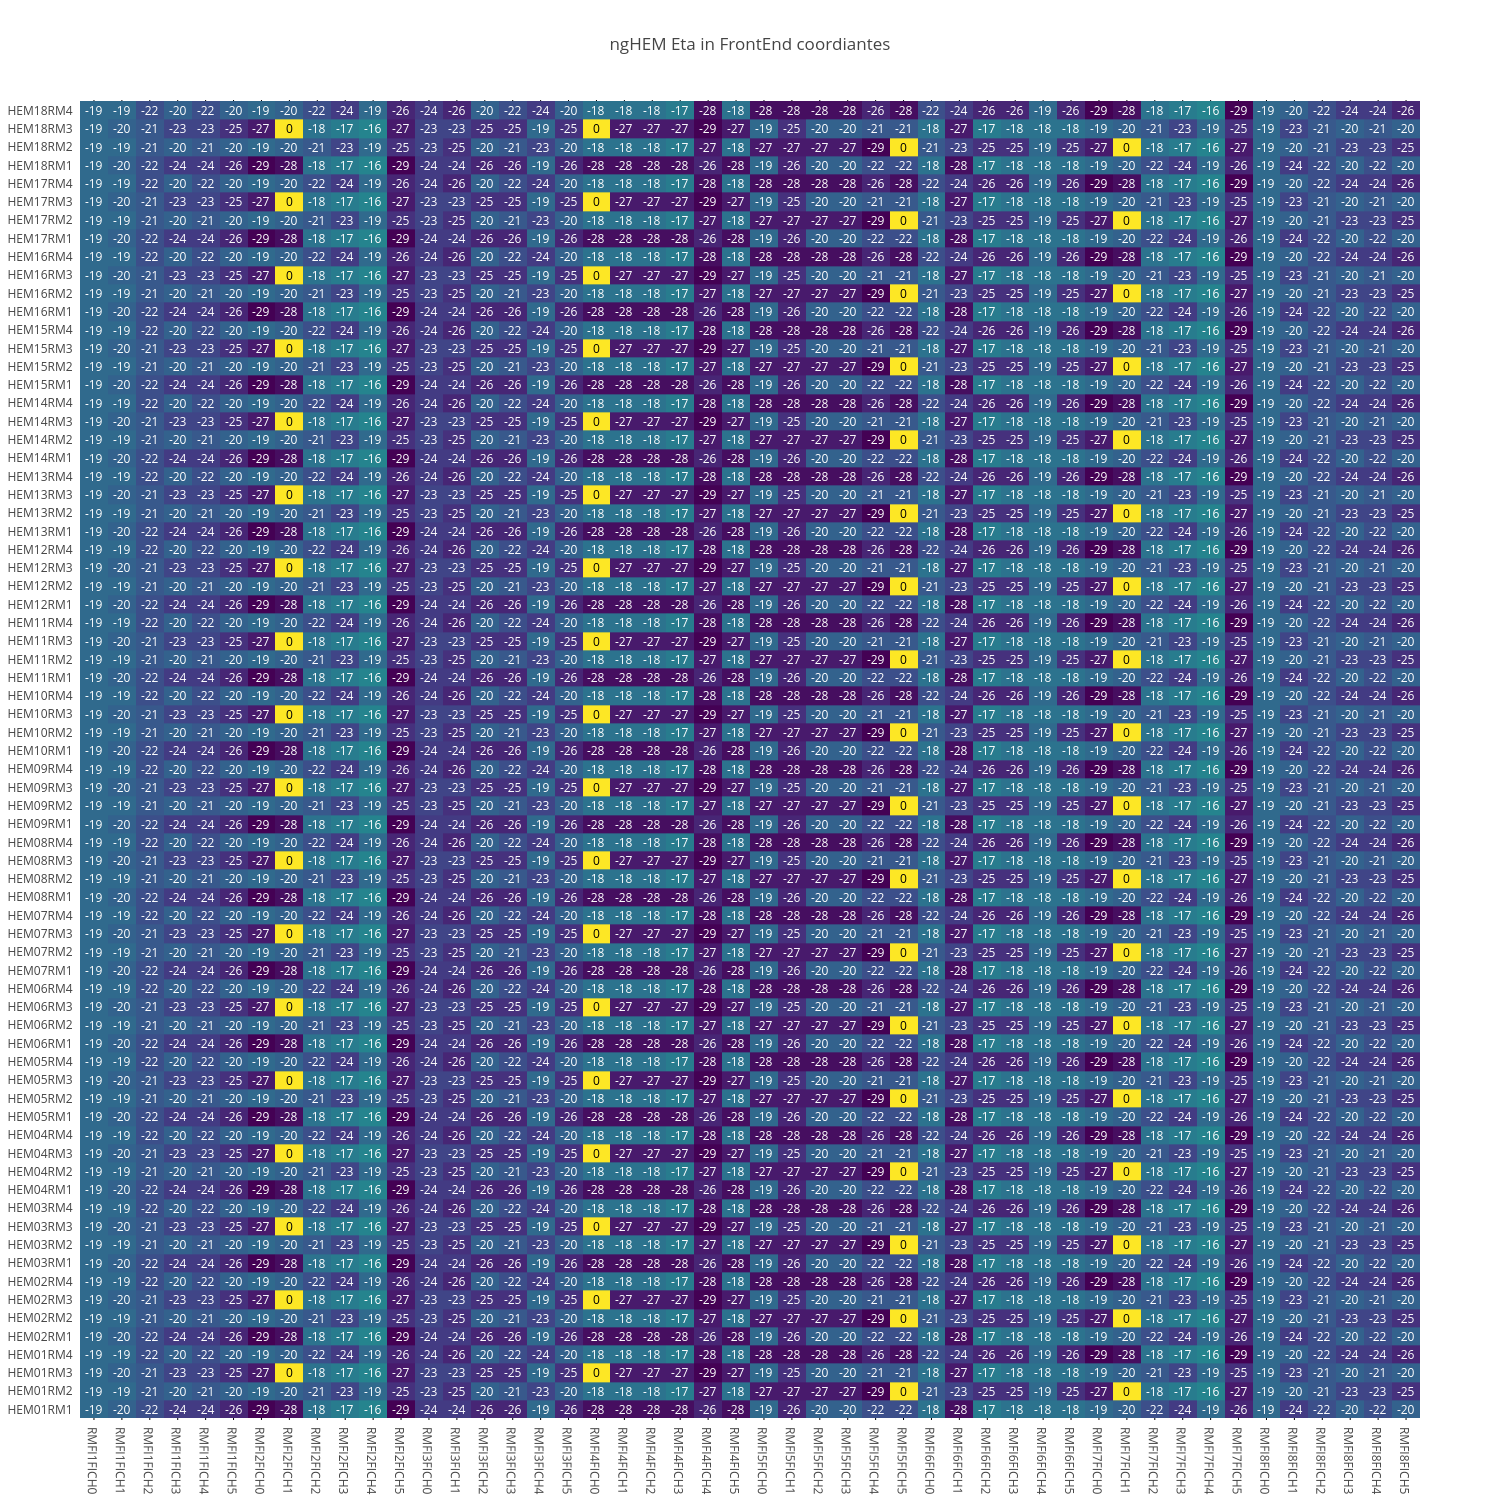
\includegraphics[angle=0,width=0.95\textwidth]{figures/appendix/ngHEM_Eta_in_FrontEnd.png}
  \end{tabular}
  \caption{HCAL (phase 1 HE, minus side) detector $\eta$ distribution in the frontend electronic coordinates.}
  \label{fig:lmapngHEMEtaFEC}
 \end{center}
\end{figure}
\clearpage

\begin{figure}[htb]
 \begin{center}
  \begin{tabular}{cc}
   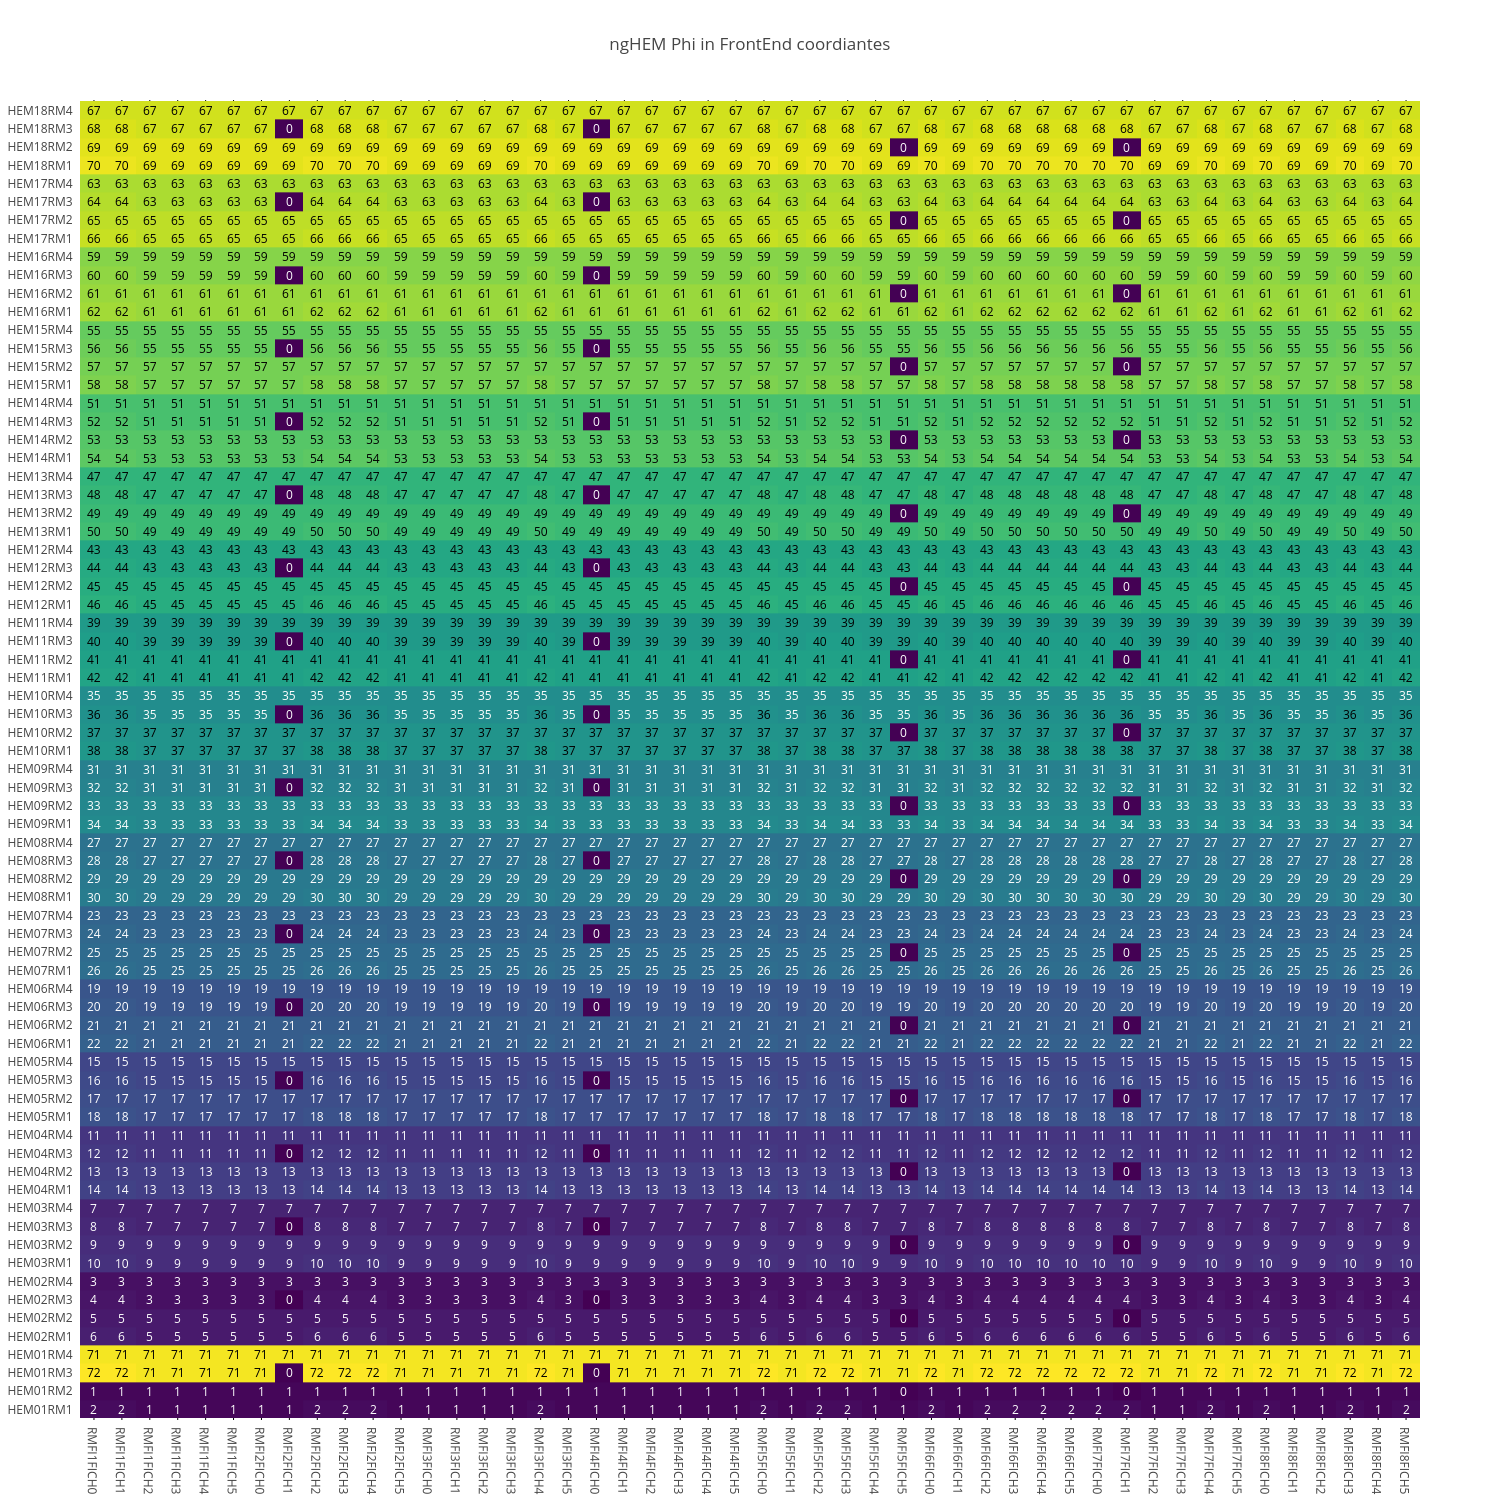
\includegraphics[angle=0,width=0.95\textwidth]{figures/appendix/ngHEM_Phi_in_FrontEnd.png}
  \end{tabular}
  \caption{HCAL (phase 1 HE, minus side) detector $\phi$ distribution in the frontend electronic coordinates.}
  \label{fig:lmapngHEMPhiFEC}
 \end{center}
\end{figure}
\clearpage

\begin{figure}[htb]
 \begin{center}
  \begin{tabular}{cc}
   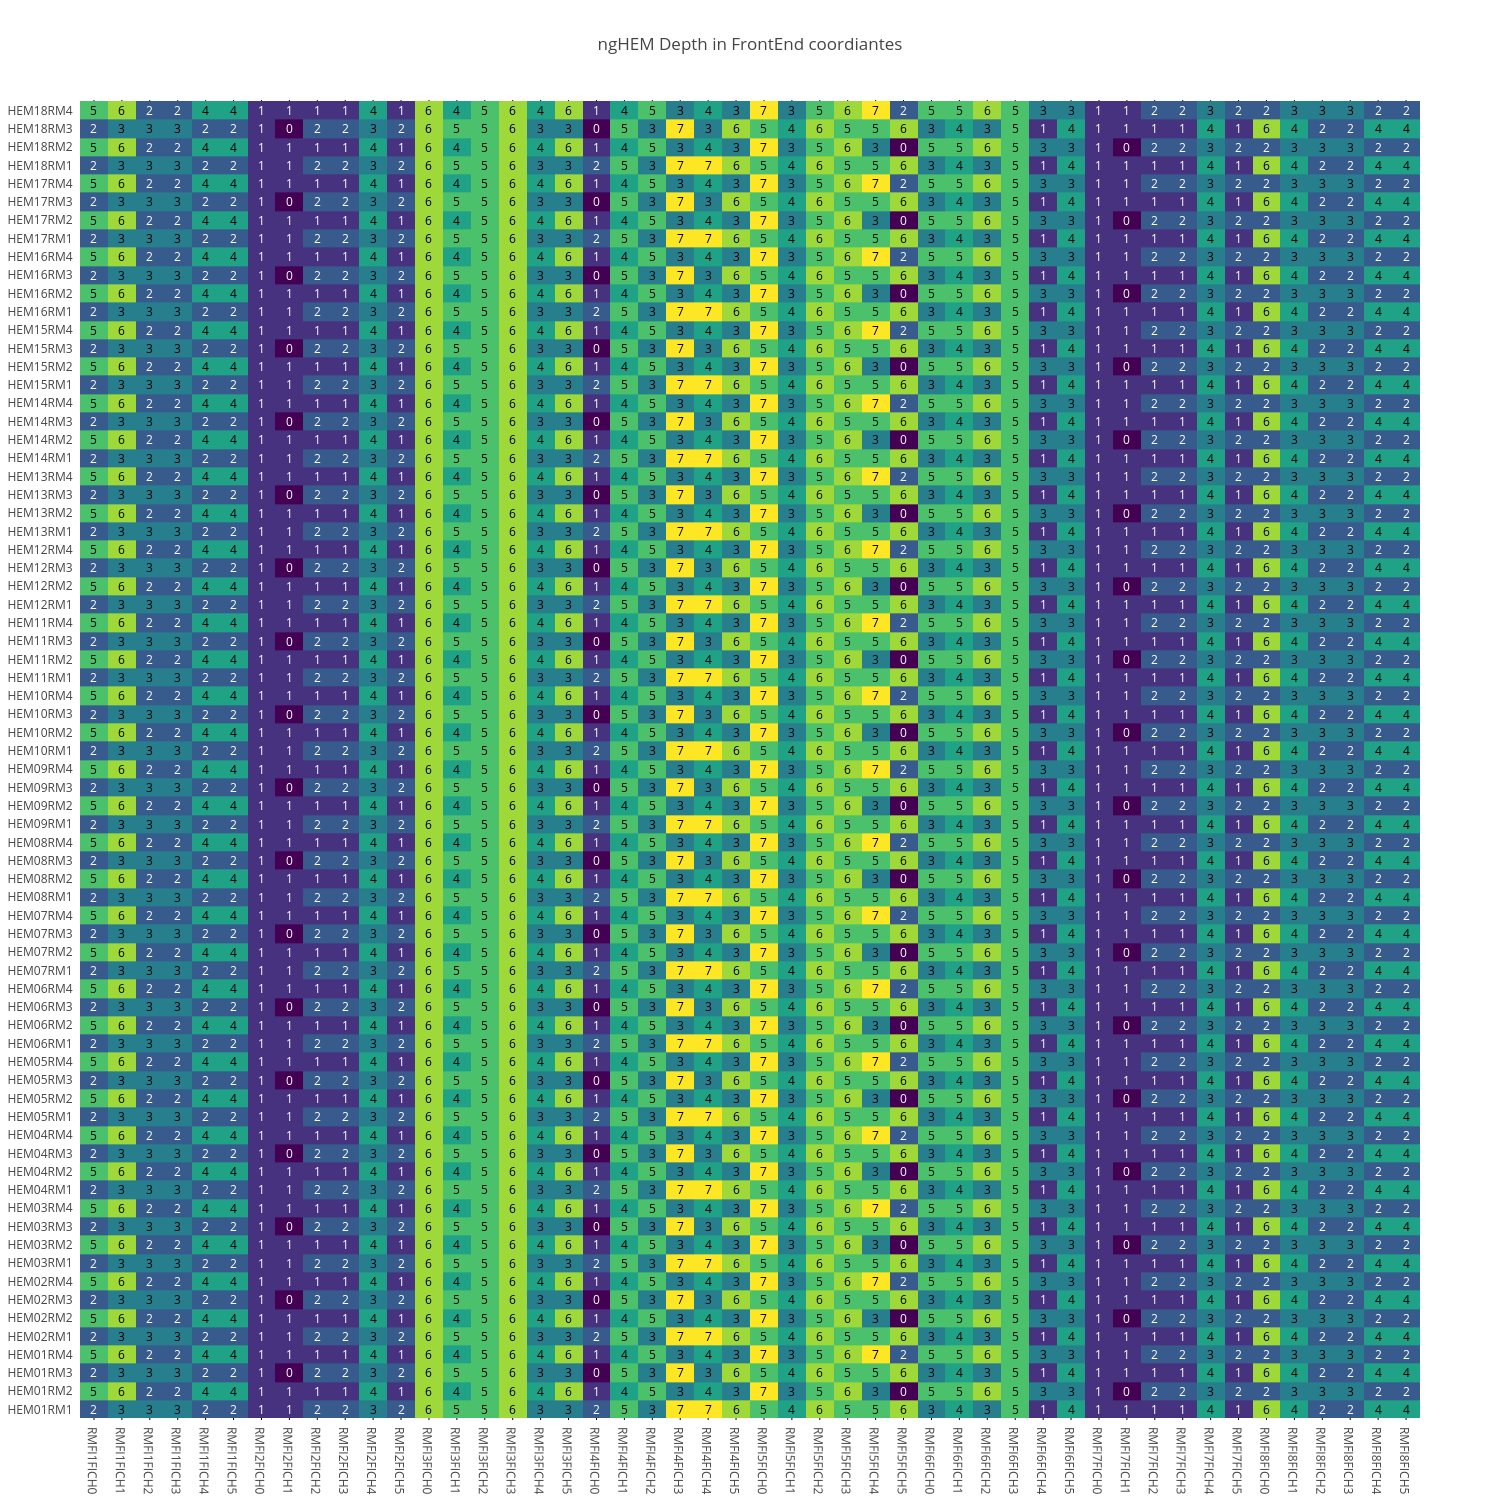
\includegraphics[angle=0,width=0.95\textwidth]{figures/appendix/ngHEM_Depth_in_FrontEnd.png}
  \end{tabular}
  \caption{HCAL (phase 1 HE, minus side) detector depth distribution in the frontend electronic coordinates.}
  \label{fig:lmapngHEMDepthFEC}
 \end{center}
\end{figure}
\clearpage

\begin{figure}[htb]
 \begin{center}
  \begin{tabular}{cc}
   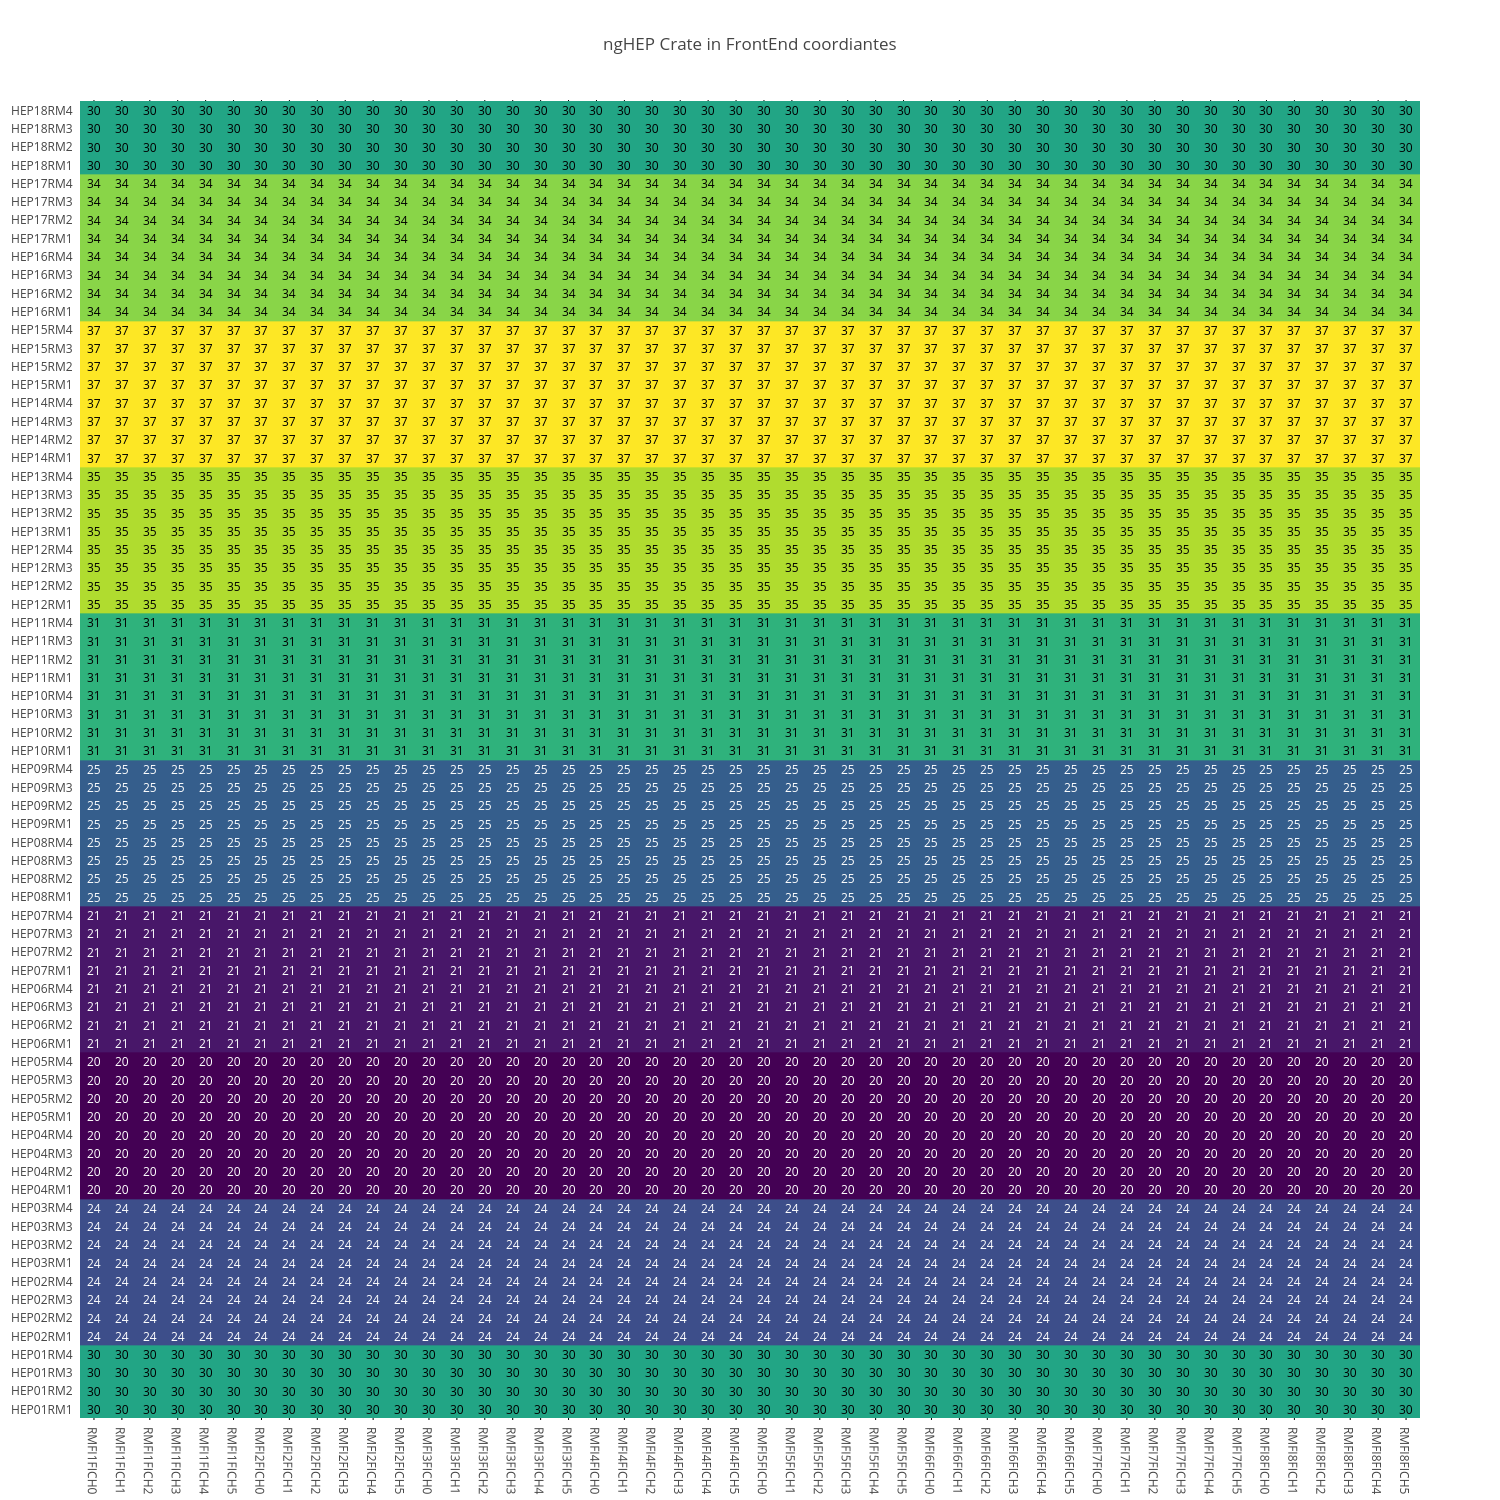
\includegraphics[angle=0,width=0.95\textwidth]{figures/appendix/ngHEP_Crate_in_FrontEnd.png}
  \end{tabular}
  \caption{HCAL (phase 1 HE, plus side) backend electronic coordinate crate distribution in the frontend electronic coordinates.}
  \label{fig:lmapngHEPCrateFEC}
 \end{center}
\end{figure}
\clearpage

\begin{figure}[htb]
 \begin{center}
  \begin{tabular}{cc}
   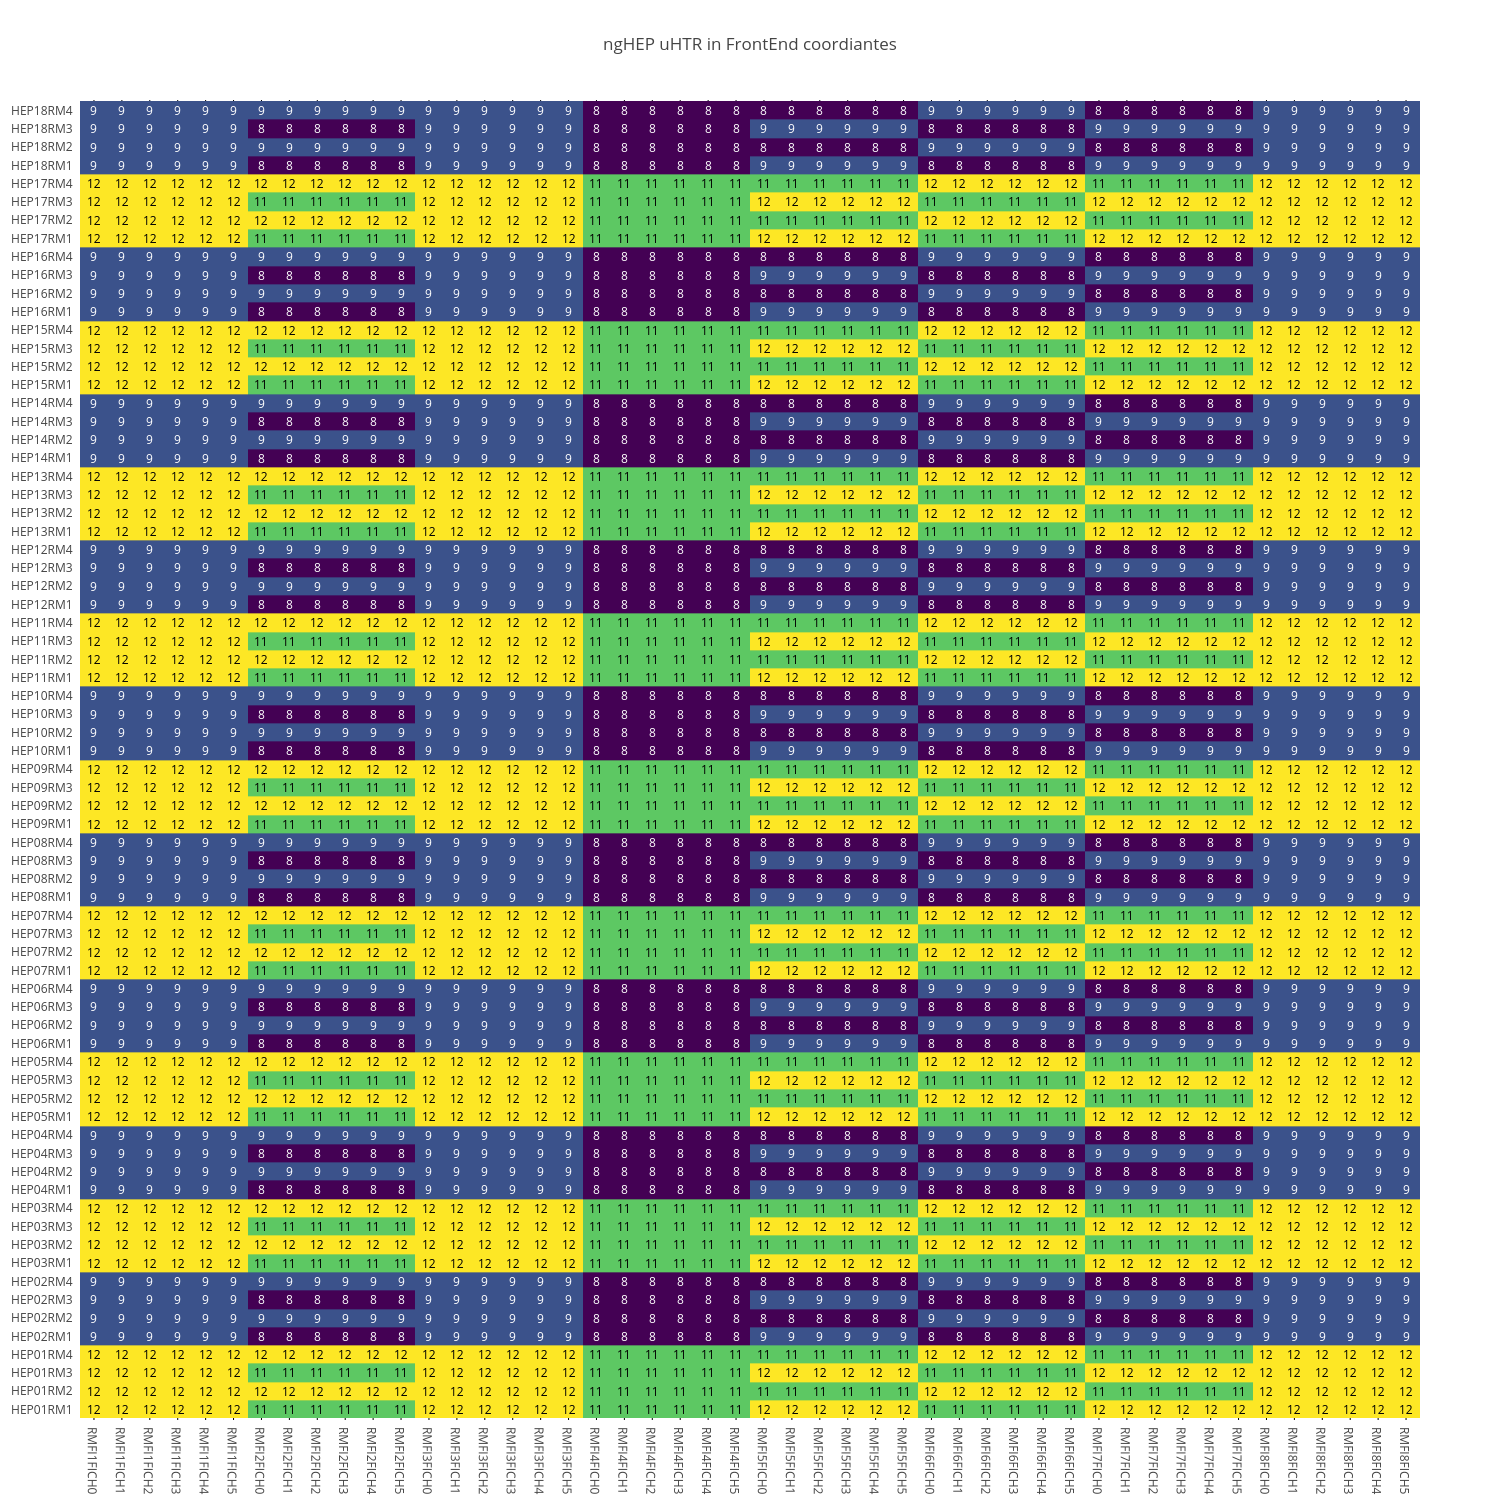
\includegraphics[angle=0,width=0.95\textwidth]{figures/appendix/ngHEP_uHTR_in_FrontEnd.png}
  \end{tabular}
  \caption{HCAL (phase 1 HE, plus side) backend electronic coordinate uHTR slot distribution in the frontend electronic coordinates.}
  \label{fig:lmapngHEPuHTRFEC}
 \end{center}
\end{figure}
\clearpage

\begin{figure}[htb]
 \begin{center}
  \begin{tabular}{cc}
   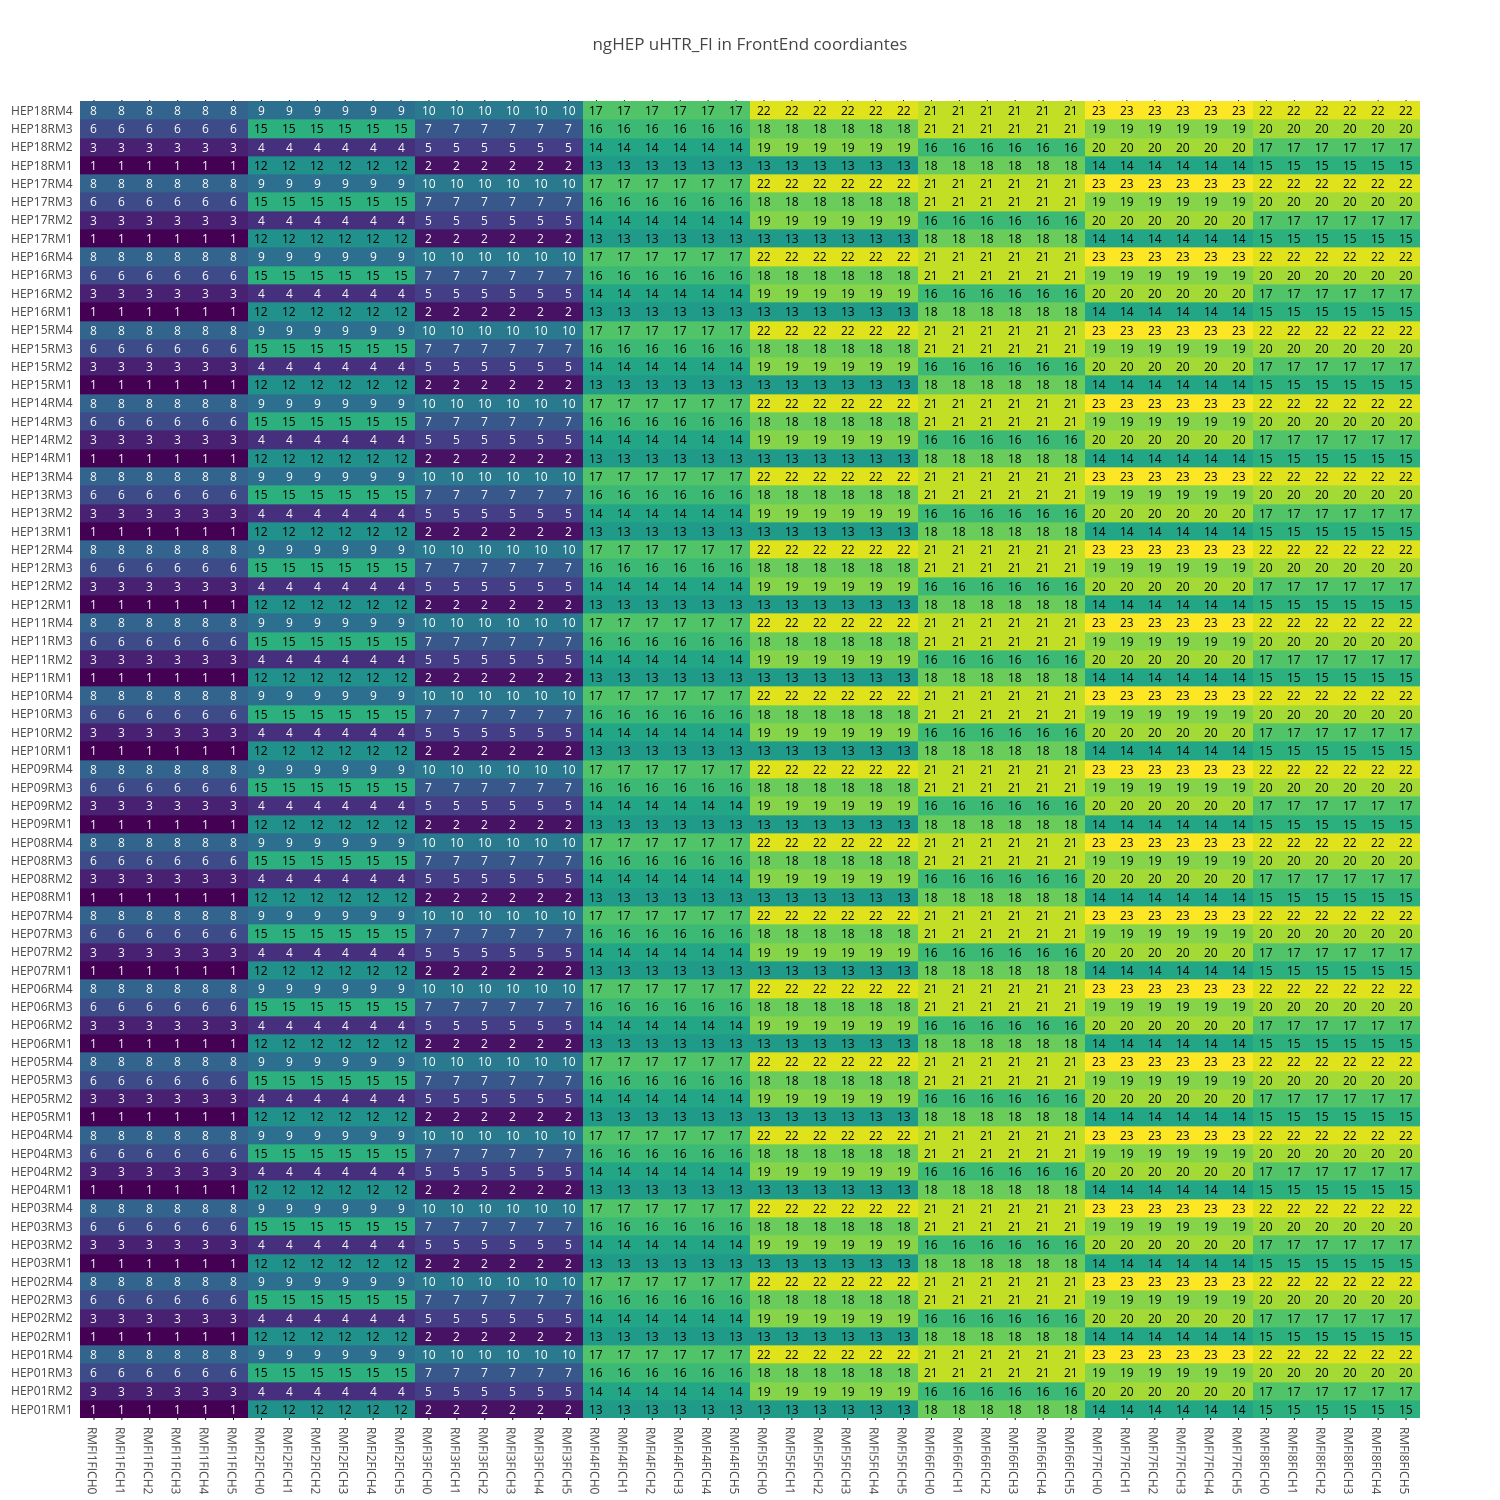
\includegraphics[angle=0,width=0.95\textwidth]{figures/appendix/ngHEP_uHTR_FI_in_FrontEnd.png}
  \end{tabular}
  \caption{HCAL (phase 1 HE, plus side) backend electronic coordinate uHTR fiber distribution in the frontend electronic coordinates.}
  \label{fig:lmapngHEPuHTRFIFEC}
 \end{center}
\end{figure}
\clearpage

\begin{figure}[htb]
 \begin{center}
  \begin{tabular}{cc}
   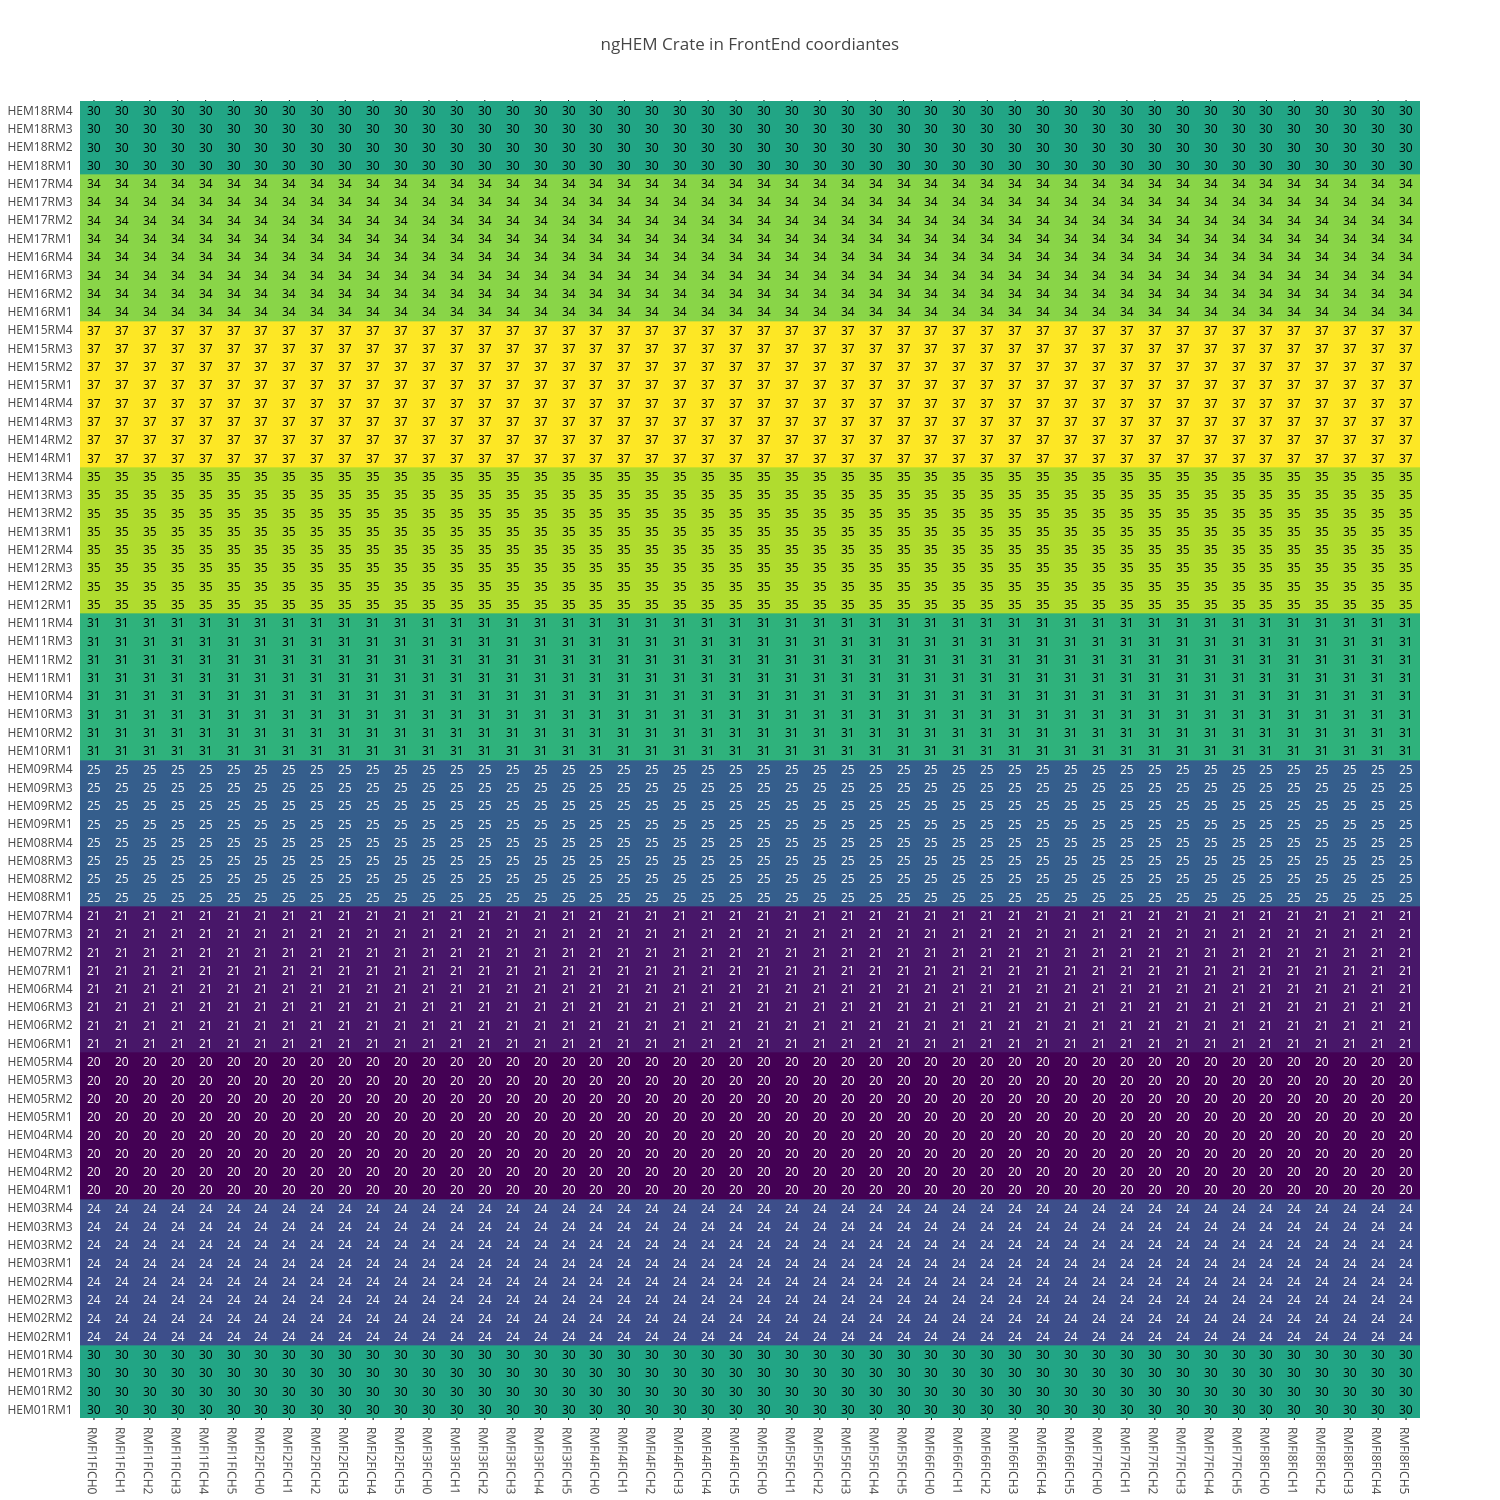
\includegraphics[angle=0,width=0.95\textwidth]{figures/appendix/ngHEM_Crate_in_FrontEnd.png}
  \end{tabular}
  \caption{HCAL (phase 1 HE, minus side) backend electronic coordinate crate distribution in the frontend electronic coordinates.}
  \label{fig:lmapngHEMCrateFEC}
 \end{center}
\end{figure}
\clearpage

\begin{figure}[htb]
 \begin{center}
  \begin{tabular}{cc}
   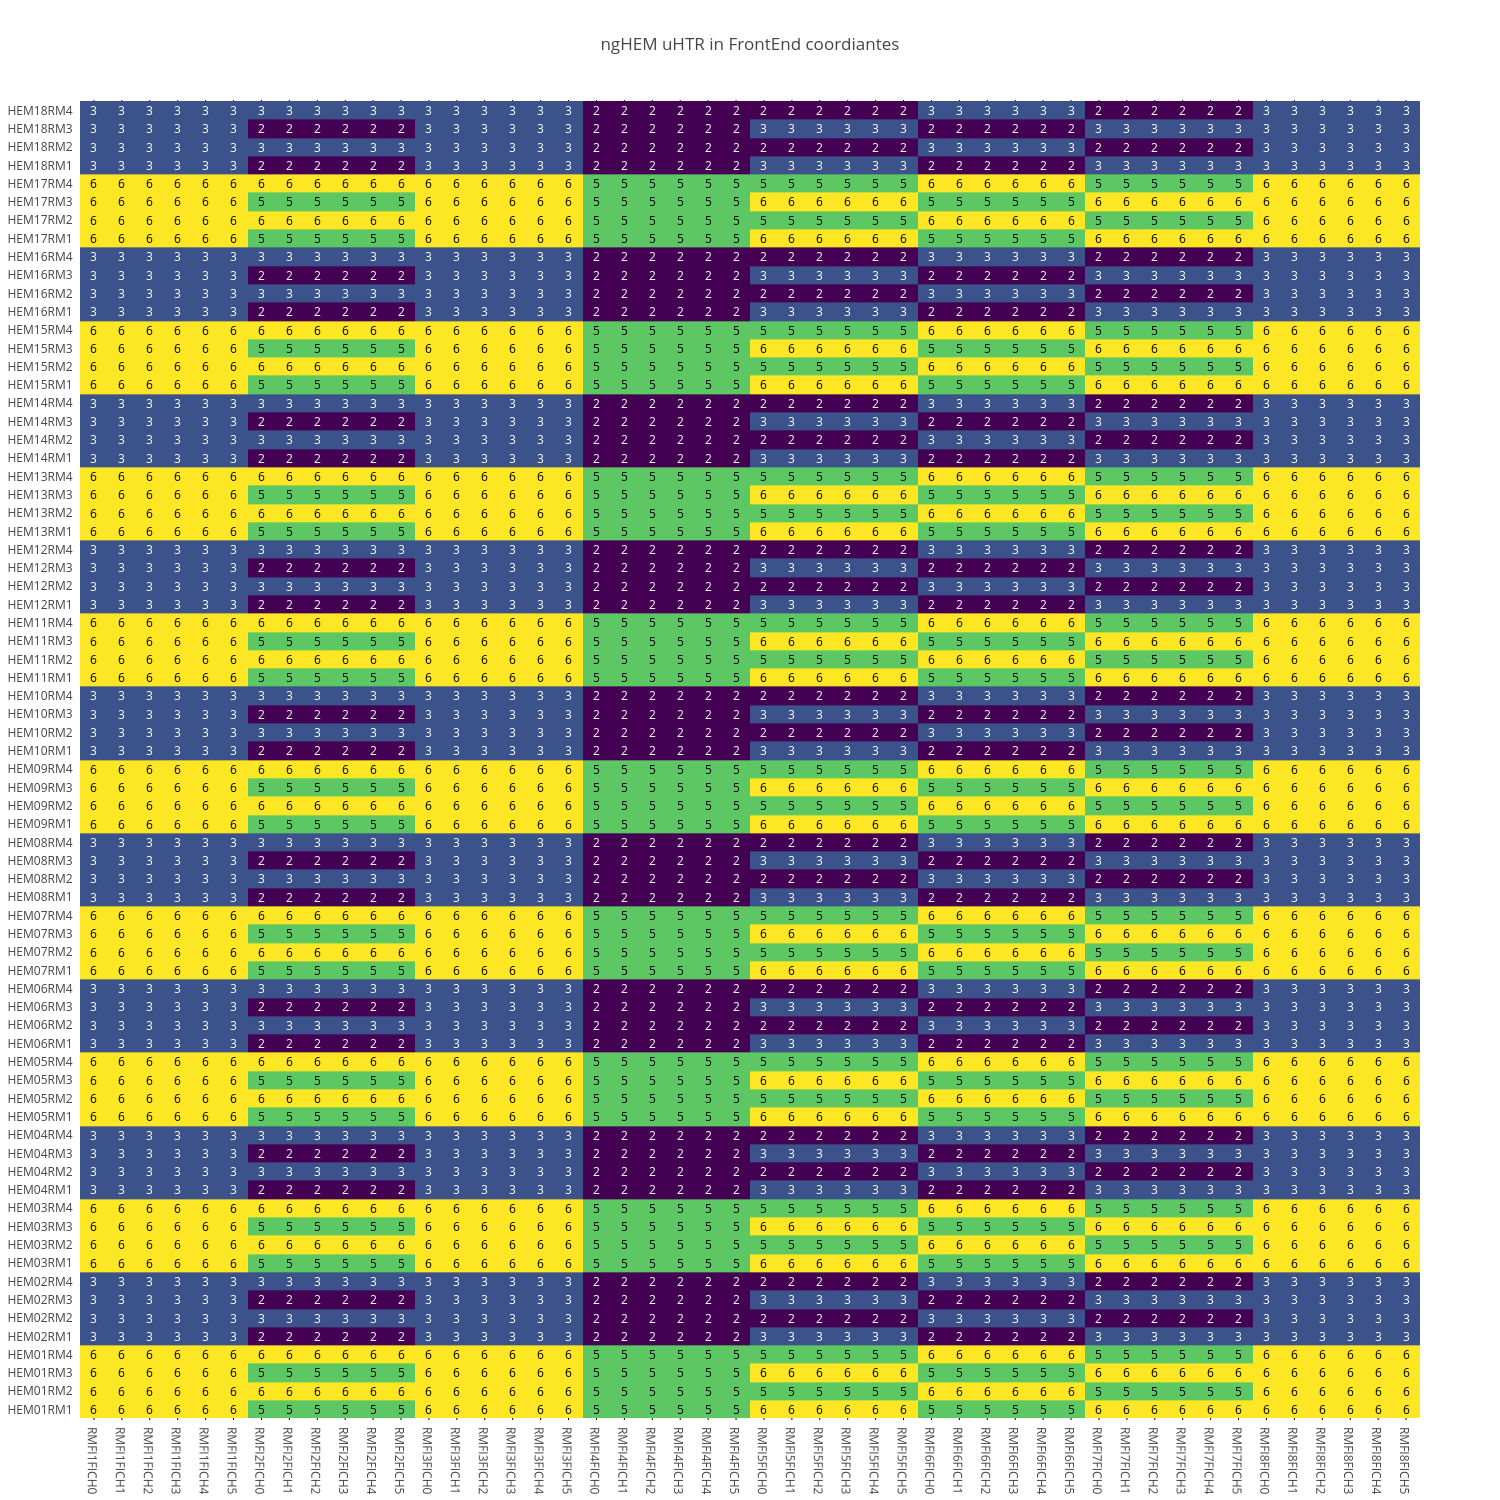
\includegraphics[angle=0,width=0.95\textwidth]{figures/appendix/ngHEM_uHTR_in_FrontEnd.png}
  \end{tabular}
  \caption{HCAL (phase 1 HE, minus side) backend electronic coordinate uHTR slot distribution in the frontend electronic coordinates.}
  \label{fig:lmapngHEMuHTRFEC}
 \end{center}
\end{figure}
\clearpage

\begin{figure}[htb]
 \begin{center}
  \begin{tabular}{cc}
   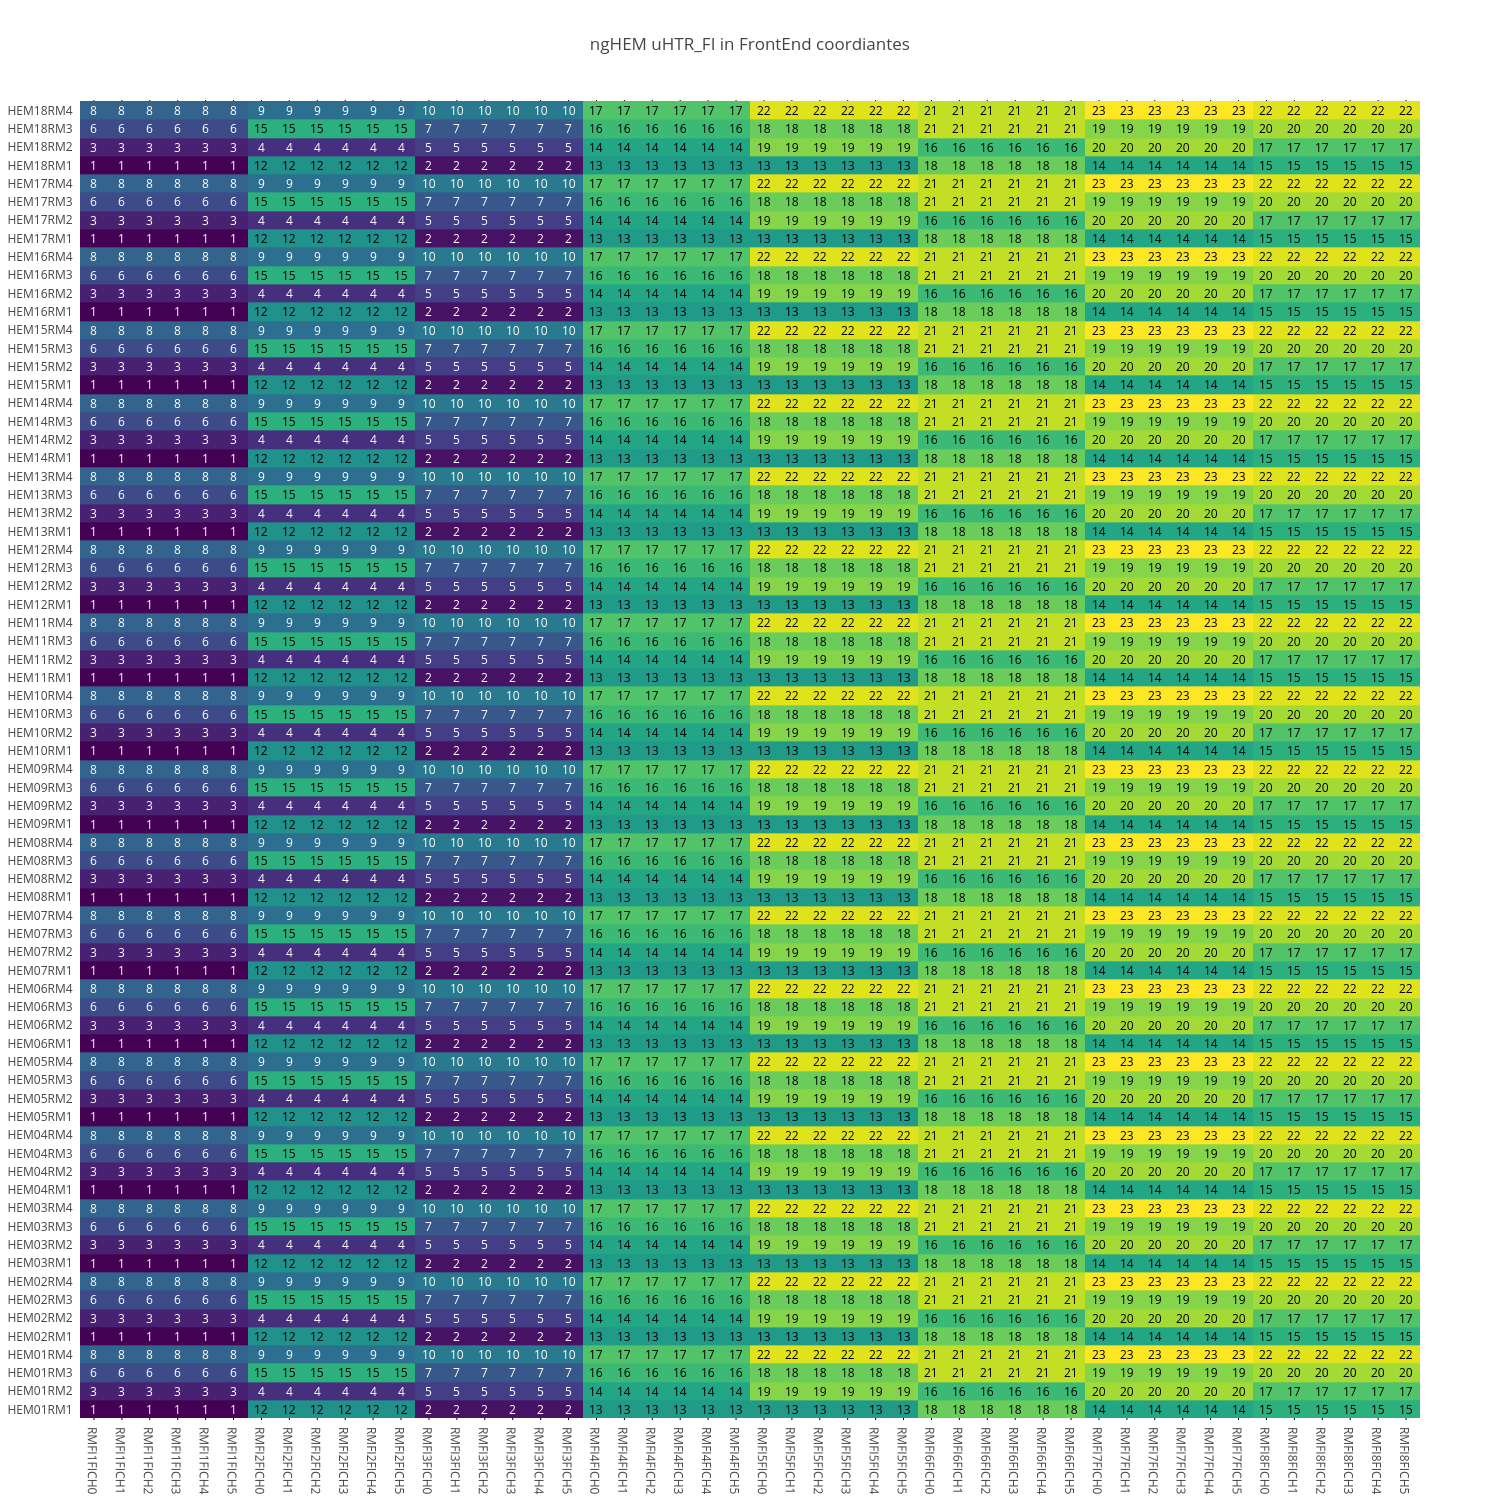
\includegraphics[angle=0,width=0.95\textwidth]{figures/appendix/ngHEM_uHTR_FI_in_FrontEnd.png}
  \end{tabular}
  \caption{HCAL (phase 1 HE, minus side) backend electronic coordinate uHTR fiber distribution in the frontend electronic coordinates.}
  \label{fig:lmapngHEMuHTRFIFEC}
 \end{center}
\end{figure}
\clearpage

\subsection{Phase 1 HF in 2017}
The 2017 HF is in PMT+QIE10 FrontEnd+uTCA BackEnd stage. HF BackEnd electronics are upgraded from VME to uTCA during 2015 YETS. HF is the first sub-detecor to have uTCA based BackEnd electronics installed and operated in CMS. HF The QIE10 FrontEnd electronics are installed on HF during 2017 YETS. 

The phase 1 2017 HF validation plots are shown from Fig~\ref{fig:lmapngHFPEtaFEC} to Fig~\ref{fig:lmapngHFMuHTRFIFEC}. There are 3456 readout channels in phase 1 HF. BackEnd electronics are in standard uTCA way: 12 uHTR and 24 uHTR fibers. The number of fiber channels per fiber is increased from 3 to 4 to accommodate dual readout channels, comparing with legacy HF. 
\clearpage

\begin{figure}[htb]
 \begin{center}
  \begin{tabular}{cc}
   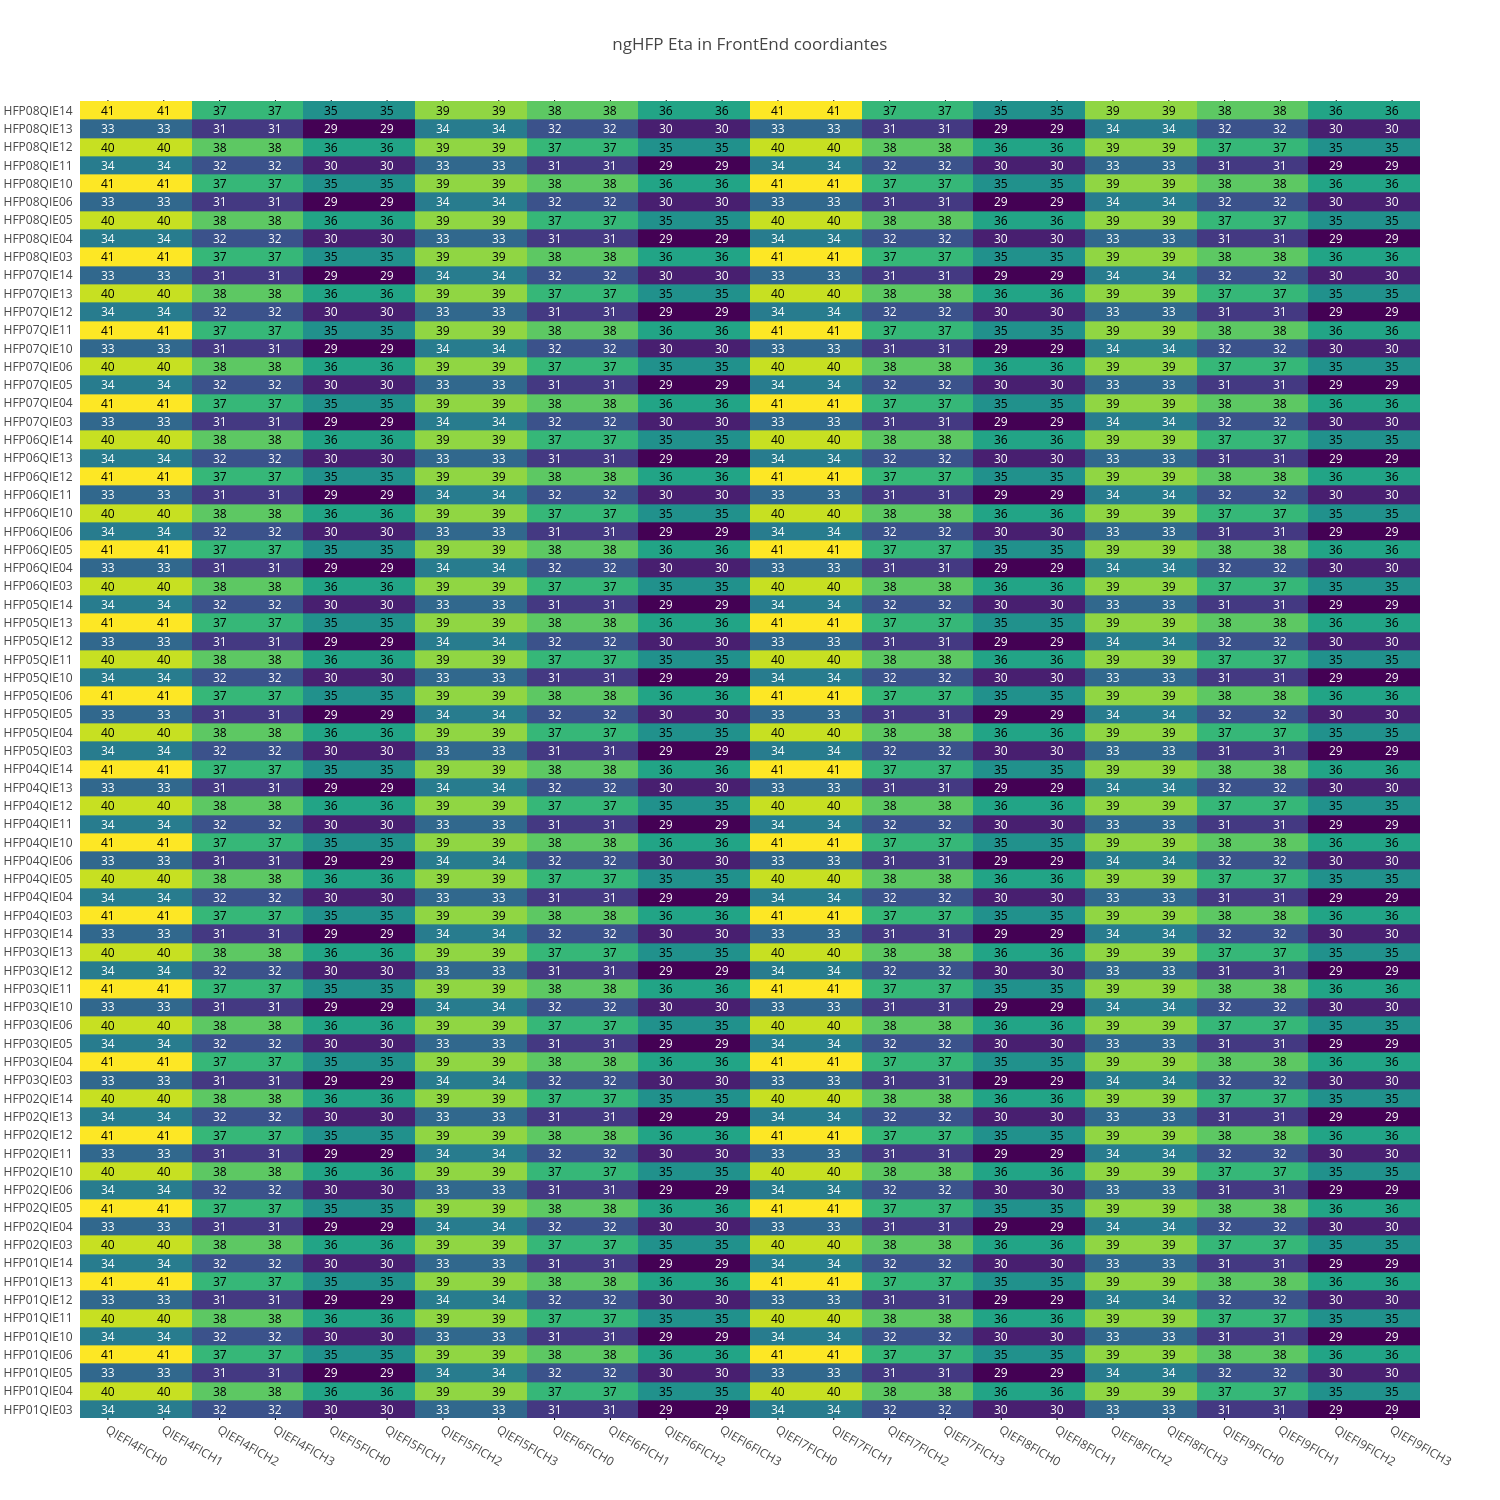
\includegraphics[angle=0,width=0.95\textwidth]{figures/appendix/ngHFP_Eta_in_FrontEnd.png}
  \end{tabular}
	\caption{HCAL (phase 1 HF, plus side) detector $\eta$ distribution in the frontend electronic coordinates.}
  \label{fig:lmapngHFPEtaFEC}
 \end{center}
\end{figure}
\clearpage

\begin{figure}[htb]
 \begin{center}
  \begin{tabular}{cc}
   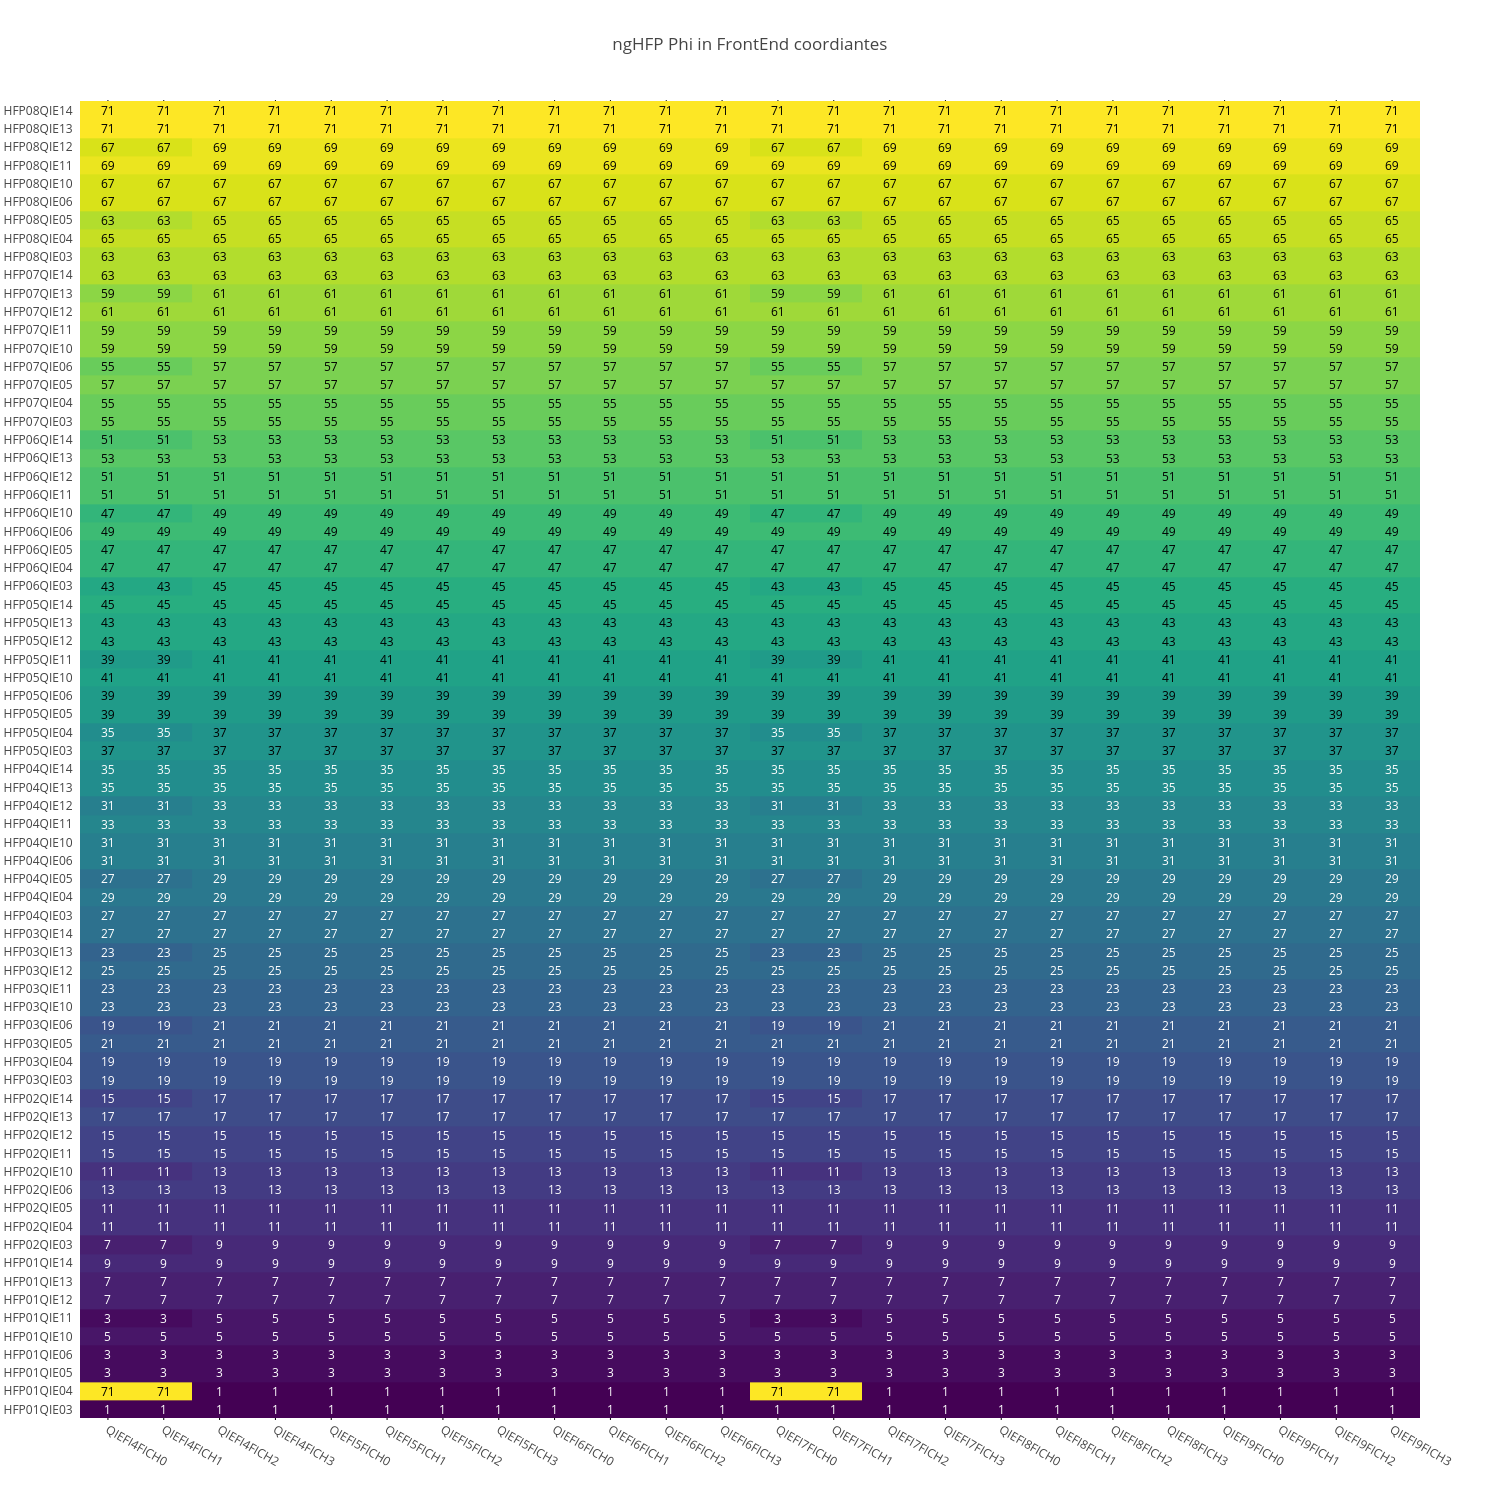
\includegraphics[angle=0,width=0.95\textwidth]{figures/appendix/ngHFP_Phi_in_FrontEnd.png}
  \end{tabular}
	\caption{HCAL (phase 1 HF, plus side) detector $\phi$ distribution in the frontend electronic coordinates.}
  \label{fig:lmapngHFPPhiFEC}
 \end{center}
\end{figure}
\clearpage

\begin{figure}[htb]
 \begin{center}
  \begin{tabular}{cc}
   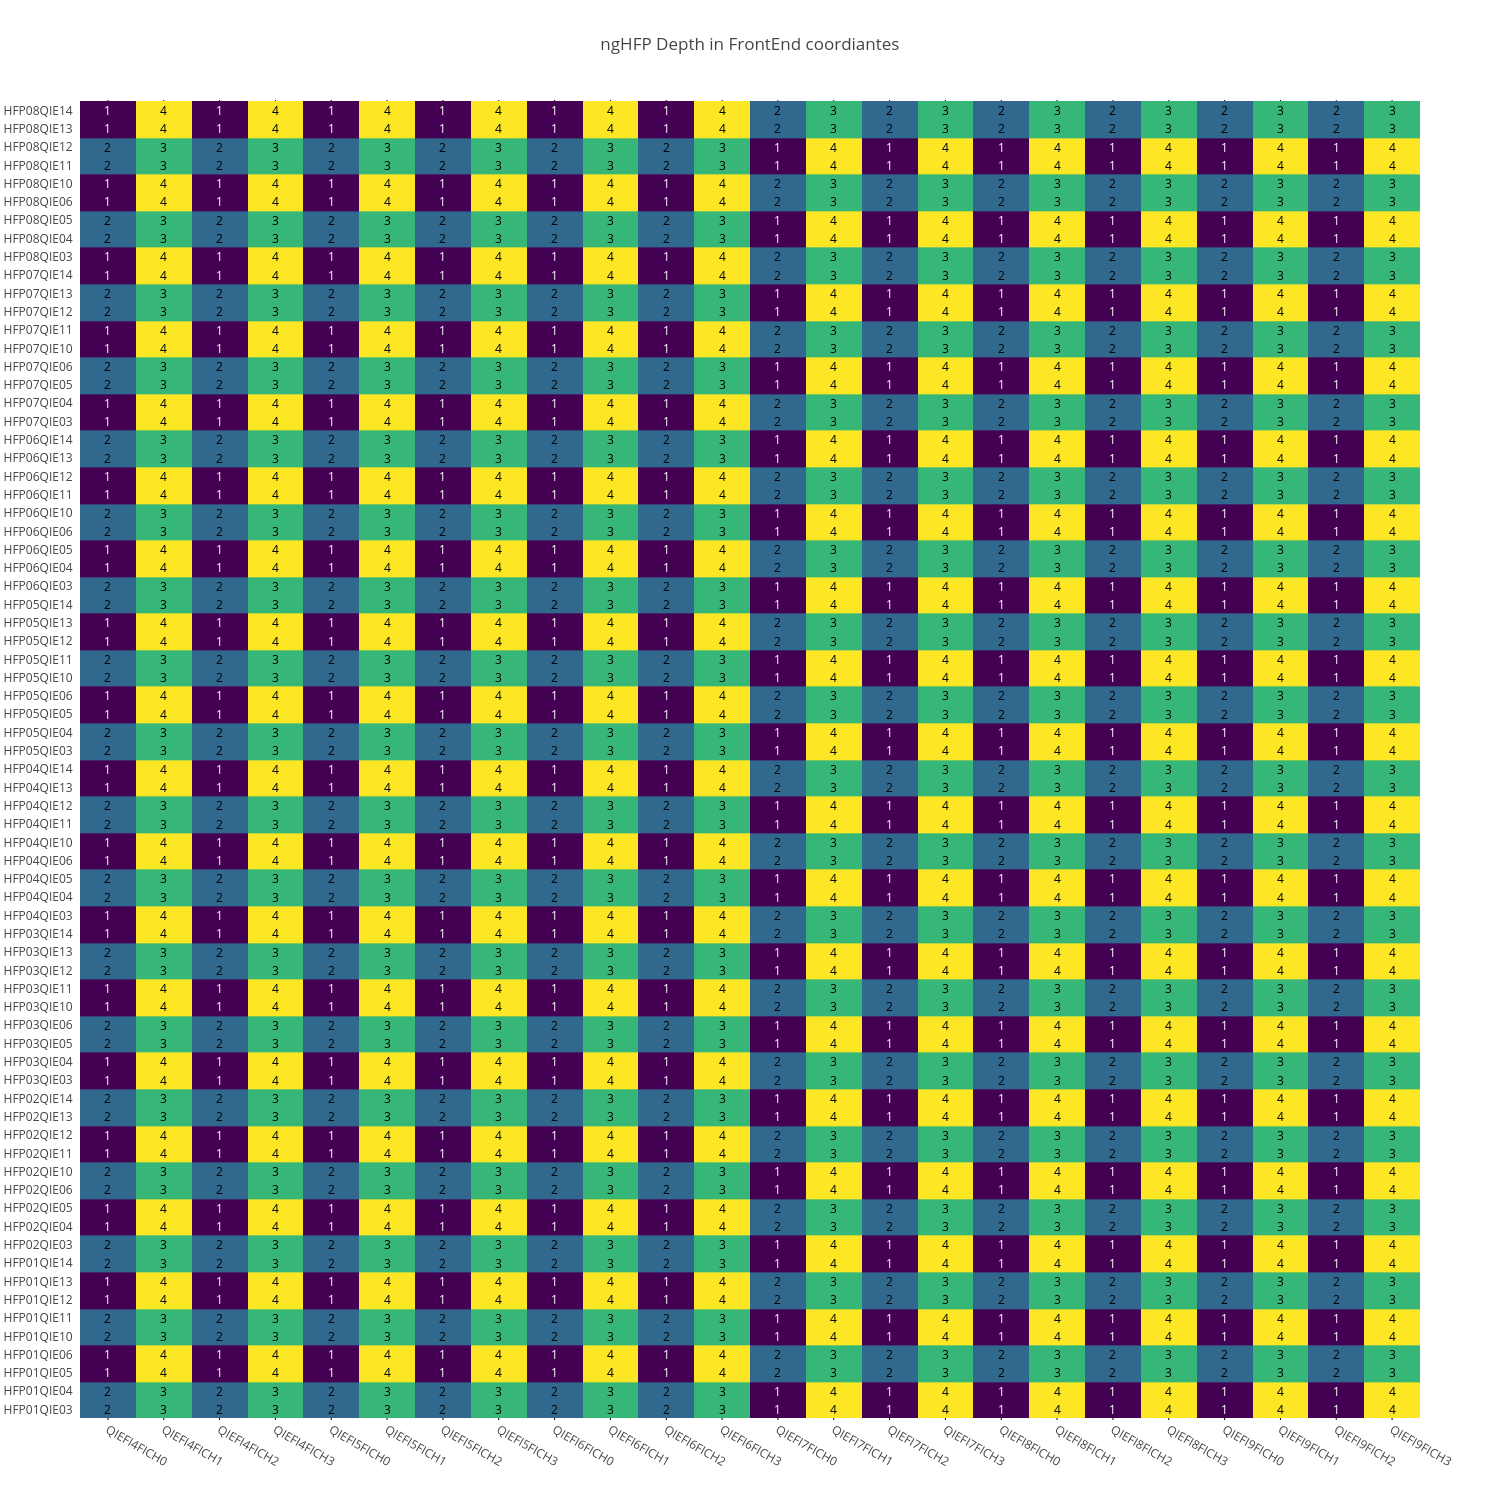
\includegraphics[angle=0,width=0.95\textwidth]{figures/appendix/ngHFP_Depth_in_FrontEnd.png}
  \end{tabular}
	\caption{HCAL (phase 1 HF, plus side) detector depth distribution in the frontend electronic coordinates.}
  \label{fig:lmapngHFPDepthFEC}
 \end{center}
\end{figure}
\clearpage

\begin{figure}[htb]
 \begin{center}
  \begin{tabular}{cc}
   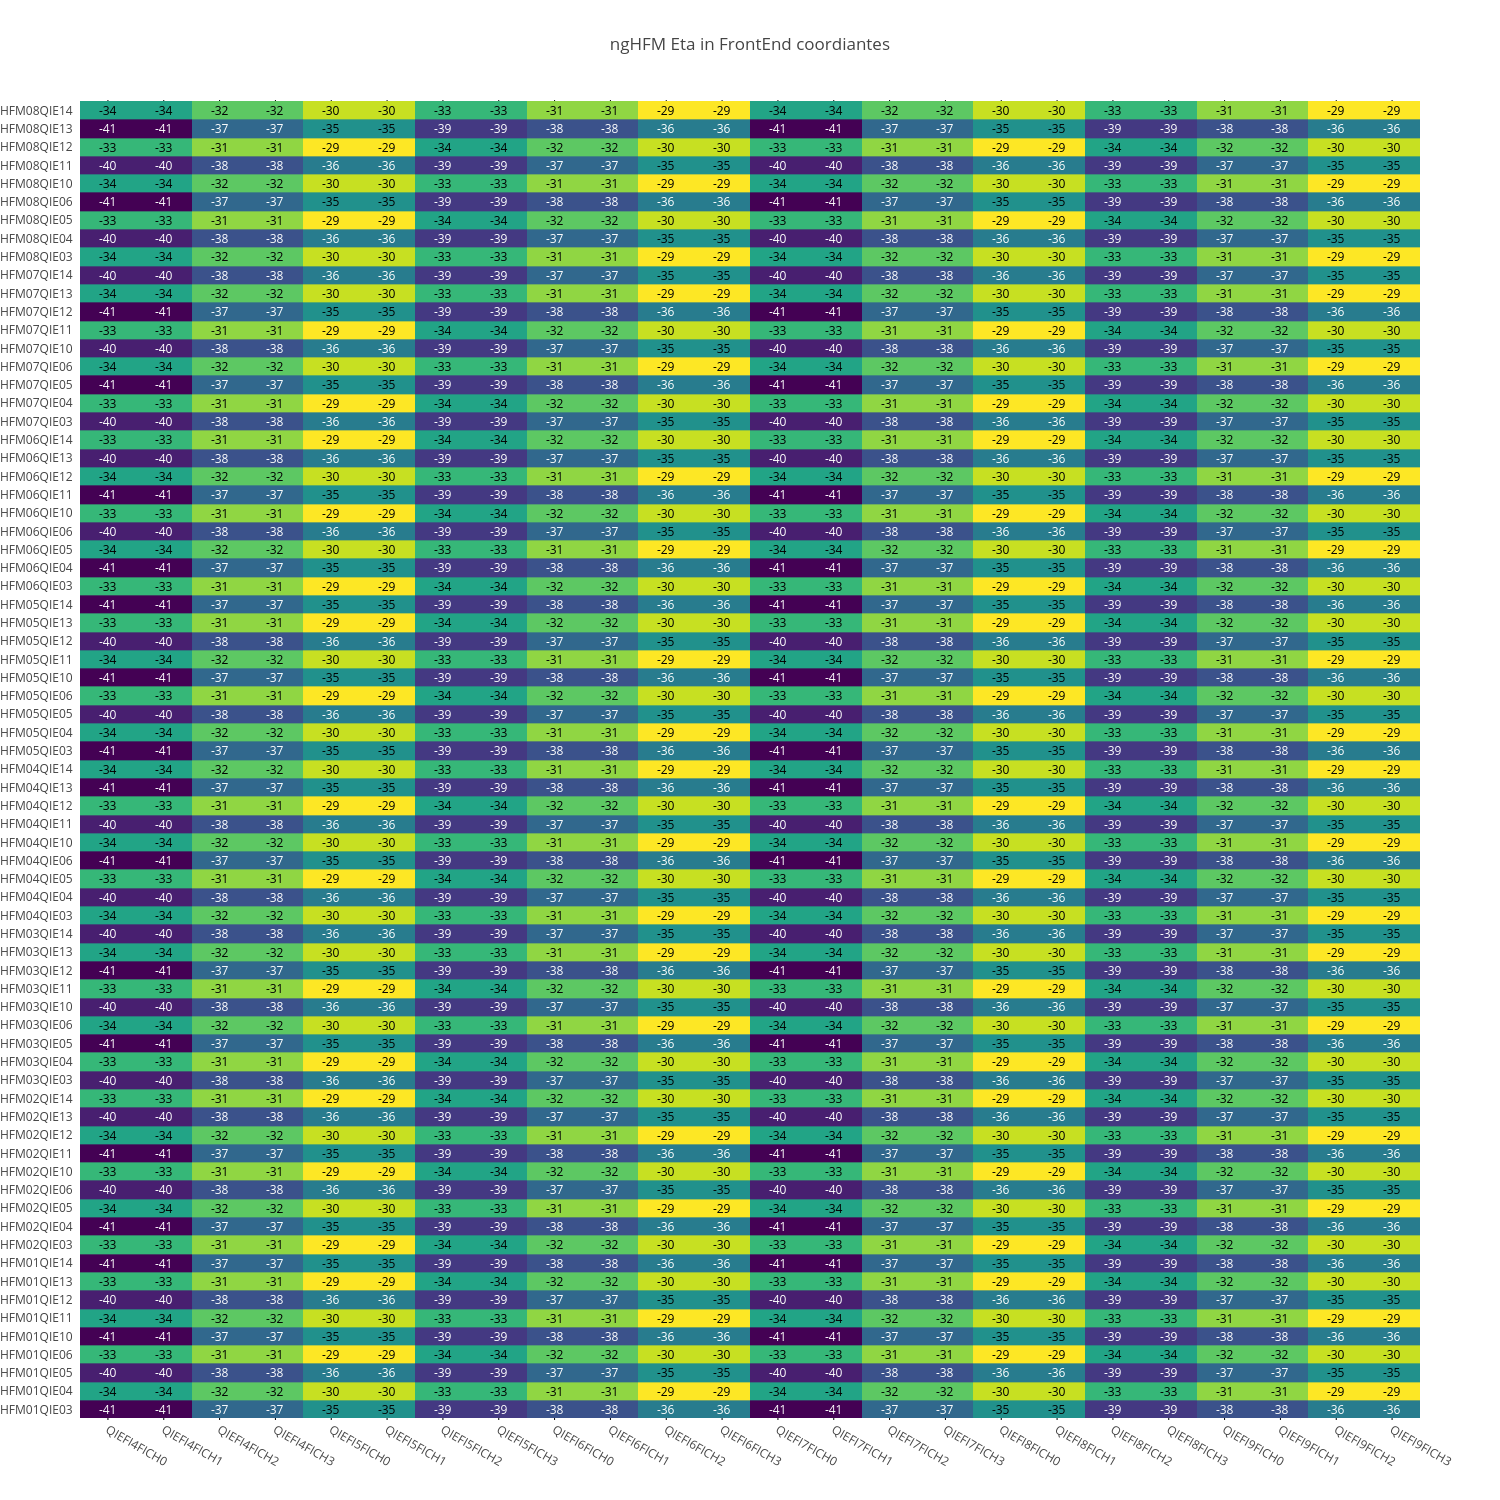
\includegraphics[angle=0,width=0.95\textwidth]{figures/appendix/ngHFM_Eta_in_FrontEnd.png}
  \end{tabular}
  \caption{HCAL (phase 1 HF, minus side) detector $\eta$ distribution in the frontend electronic coordinates.}
  \label{fig:lmapngHFMEtaFEC}
 \end{center}
\end{figure}
\clearpage

\begin{figure}[htb]
 \begin{center}
  \begin{tabular}{cc}
   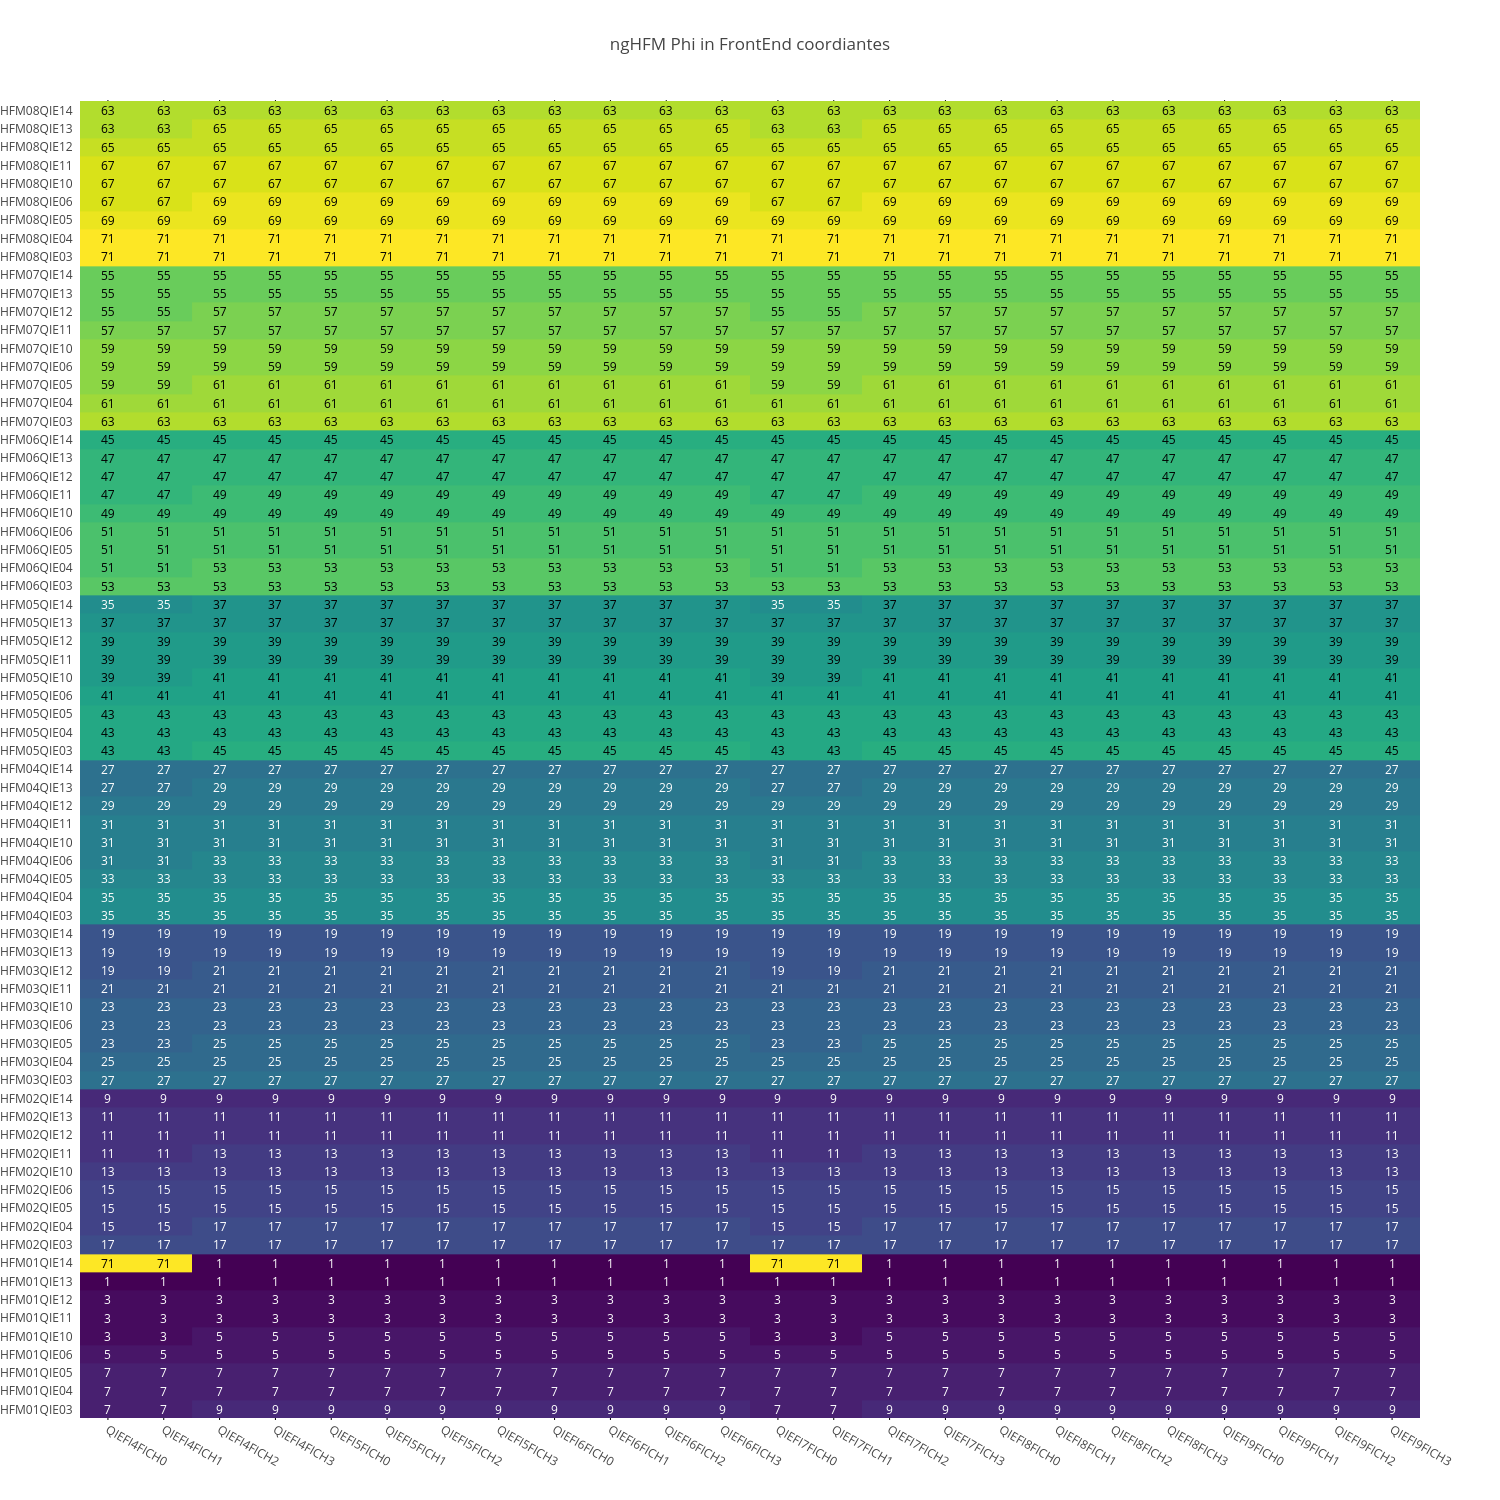
\includegraphics[angle=0,width=0.95\textwidth]{figures/appendix/ngHFM_Phi_in_FrontEnd.png}
  \end{tabular}
  \caption{HCAL (phase 1 HF, minus side) detector $\phi$ distribution in the frontend electronic coordinates.}
  \label{fig:lmapngHFMPhiFEC}
 \end{center}
\end{figure}
\clearpage

\begin{figure}[htb]
 \begin{center}
  \begin{tabular}{cc}
   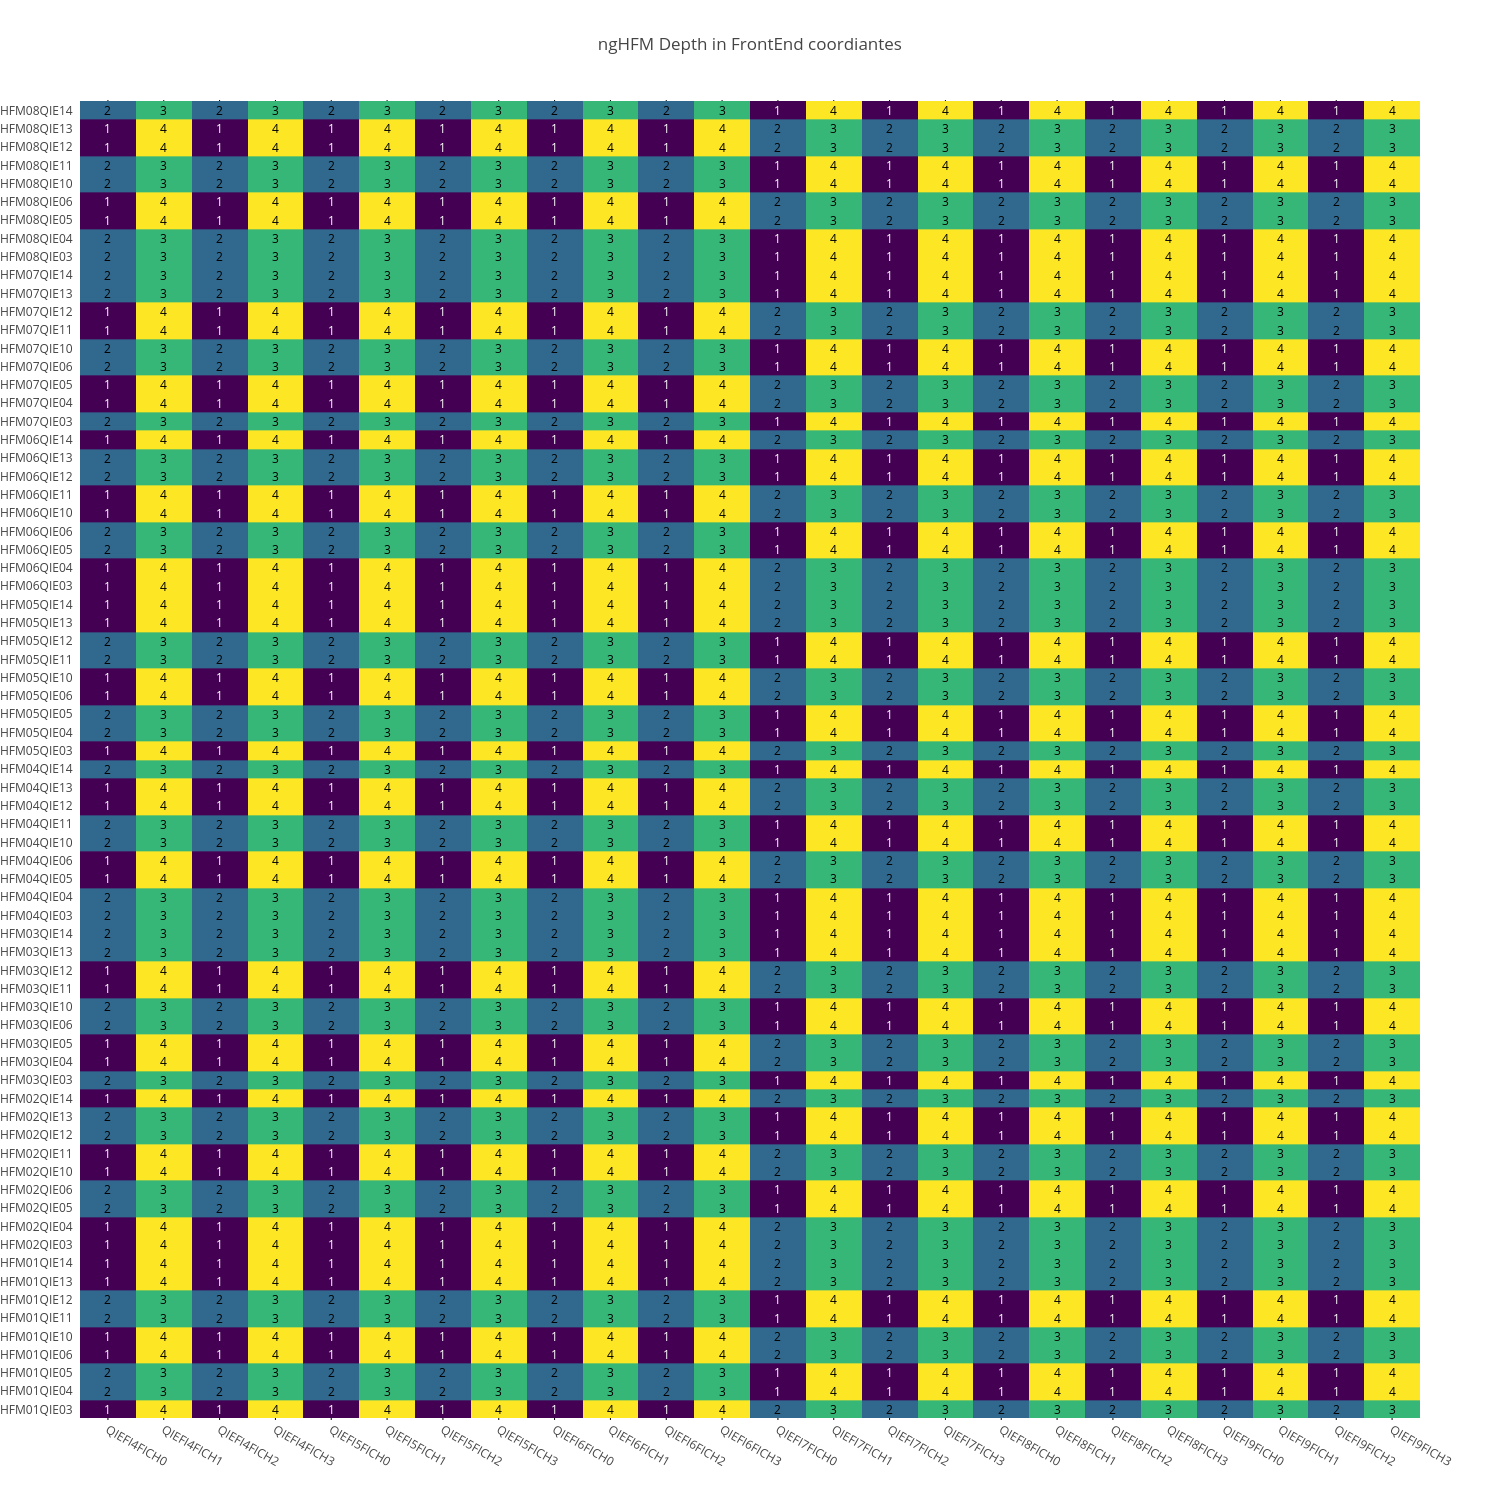
\includegraphics[angle=0,width=0.95\textwidth]{figures/appendix/ngHFM_Depth_in_FrontEnd.png}
  \end{tabular}
  \caption{HCAL (phase 1 HF, minus side) detector depth distribution in the frontend electronic coordinates.}
  \label{fig:lmapngHFMDepthFEC}
 \end{center}
\end{figure}
\clearpage

\begin{figure}[htb]
 \begin{center}
  \begin{tabular}{cc}
   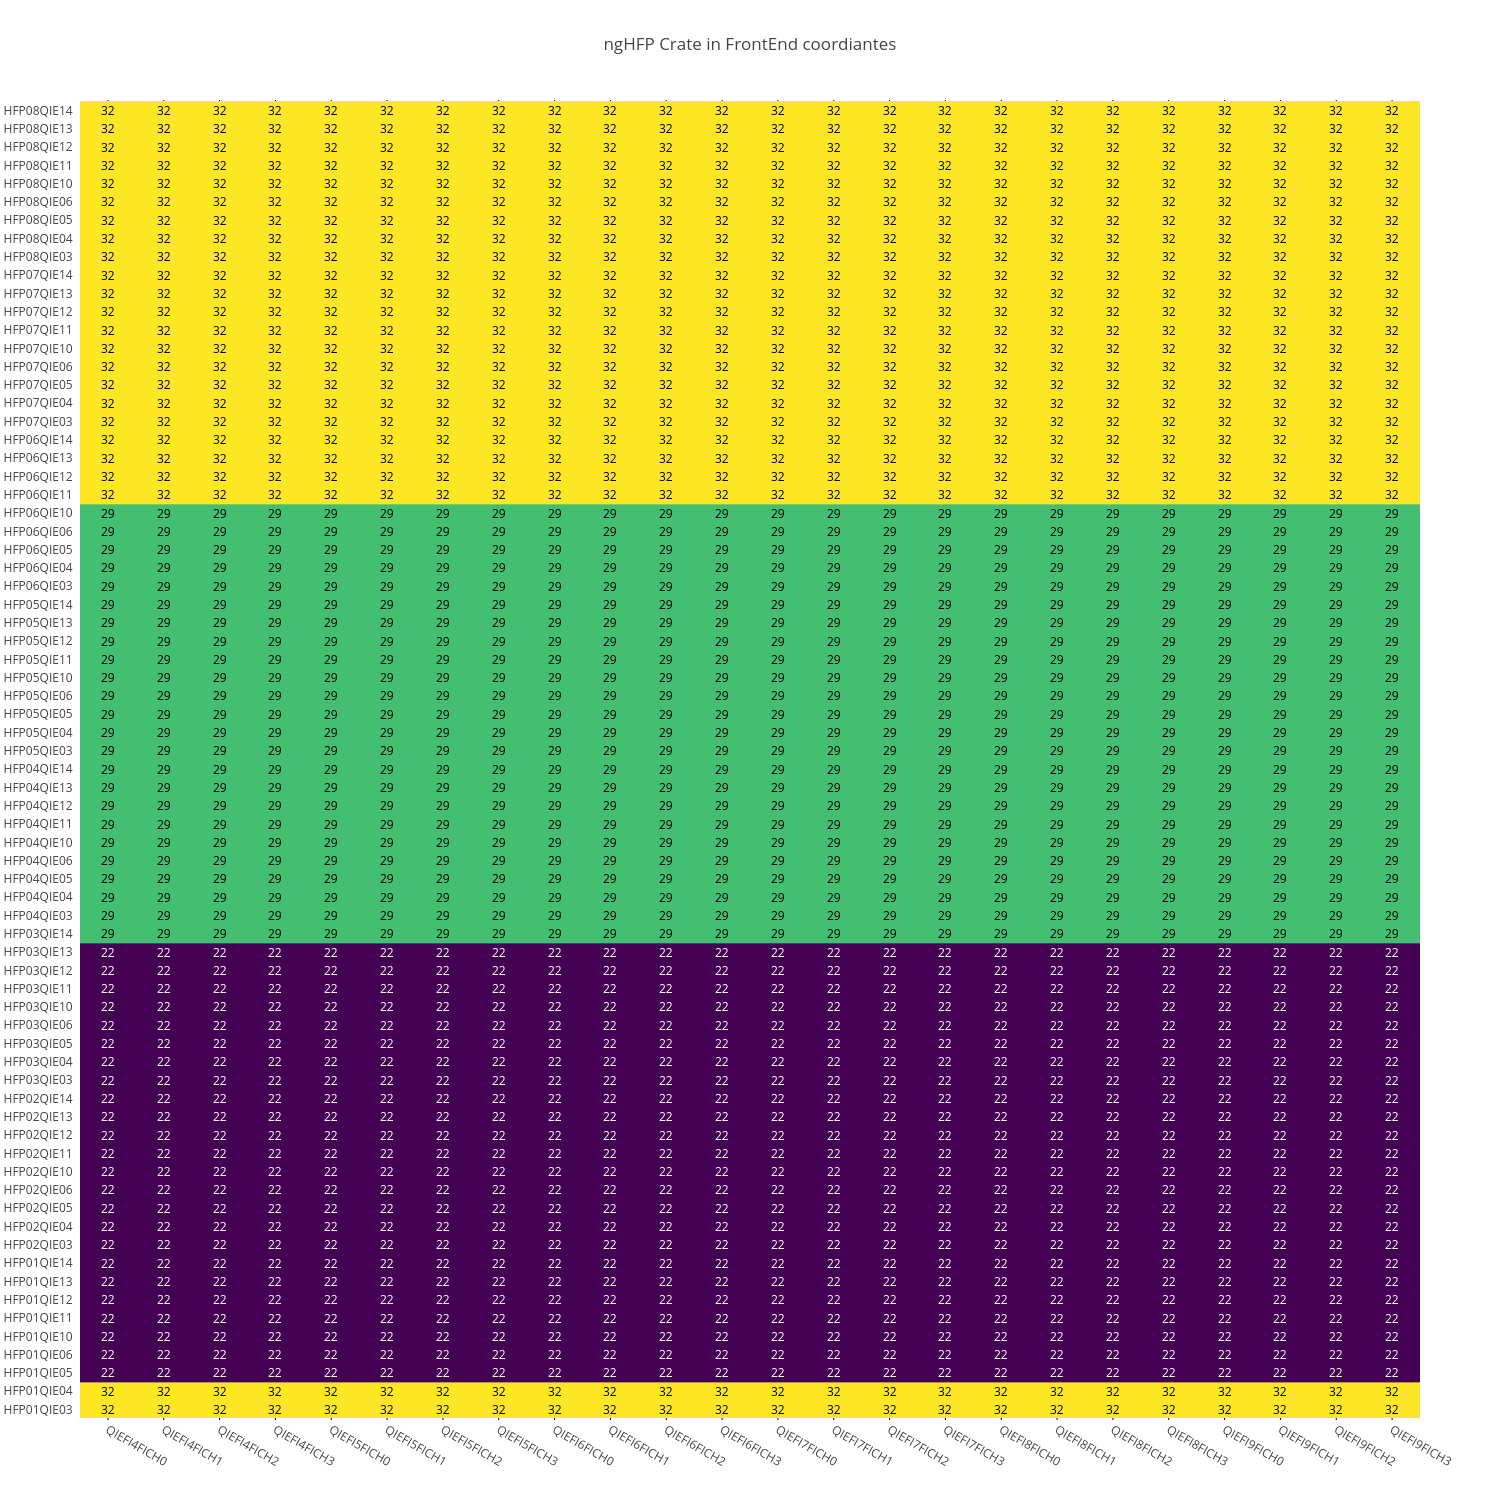
\includegraphics[angle=0,width=0.95\textwidth]{figures/appendix/ngHFP_Crate_in_FrontEnd.png}
  \end{tabular}
  \caption{HCAL (phase 1 HF, plus side) backend electronic coordinate crate distribution in the frontend electronic coordinates.}
  \label{fig:lmapngHFPCrateFEC}
 \end{center}
\end{figure}
\clearpage

\begin{figure}[htb]
 \begin{center}
  \begin{tabular}{cc}
   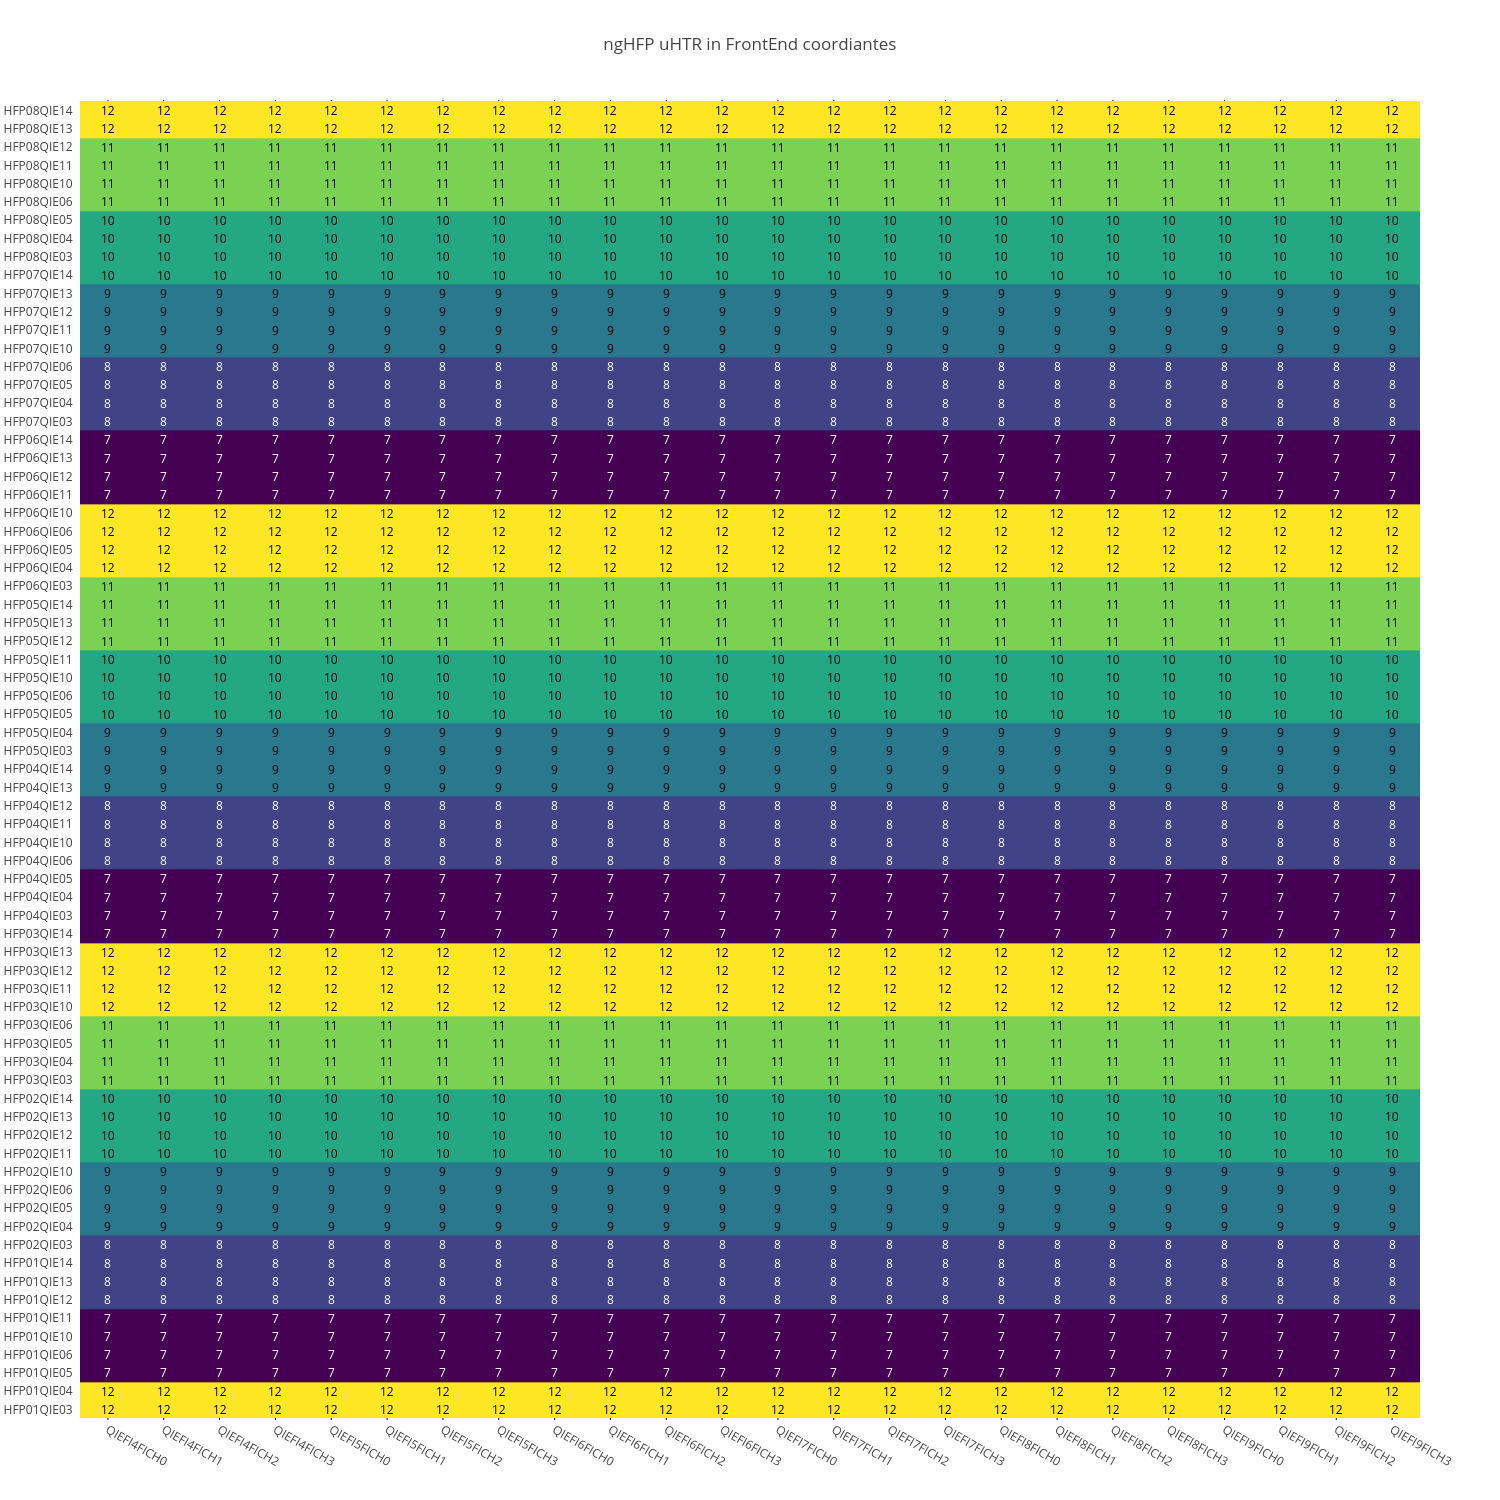
\includegraphics[angle=0,width=0.95\textwidth]{figures/appendix/ngHFP_uHTR_in_FrontEnd.png}
  \end{tabular}
  \caption{HCAL (phase 1 HF, plus side) backend electronic coordinate uHTR slot distribution in the frontend electronic coordinates.}
  \label{fig:lmapngHFPuHTRFEC}
 \end{center}
\end{figure}
\clearpage

\begin{figure}[htb]
 \begin{center}
  \begin{tabular}{cc}
   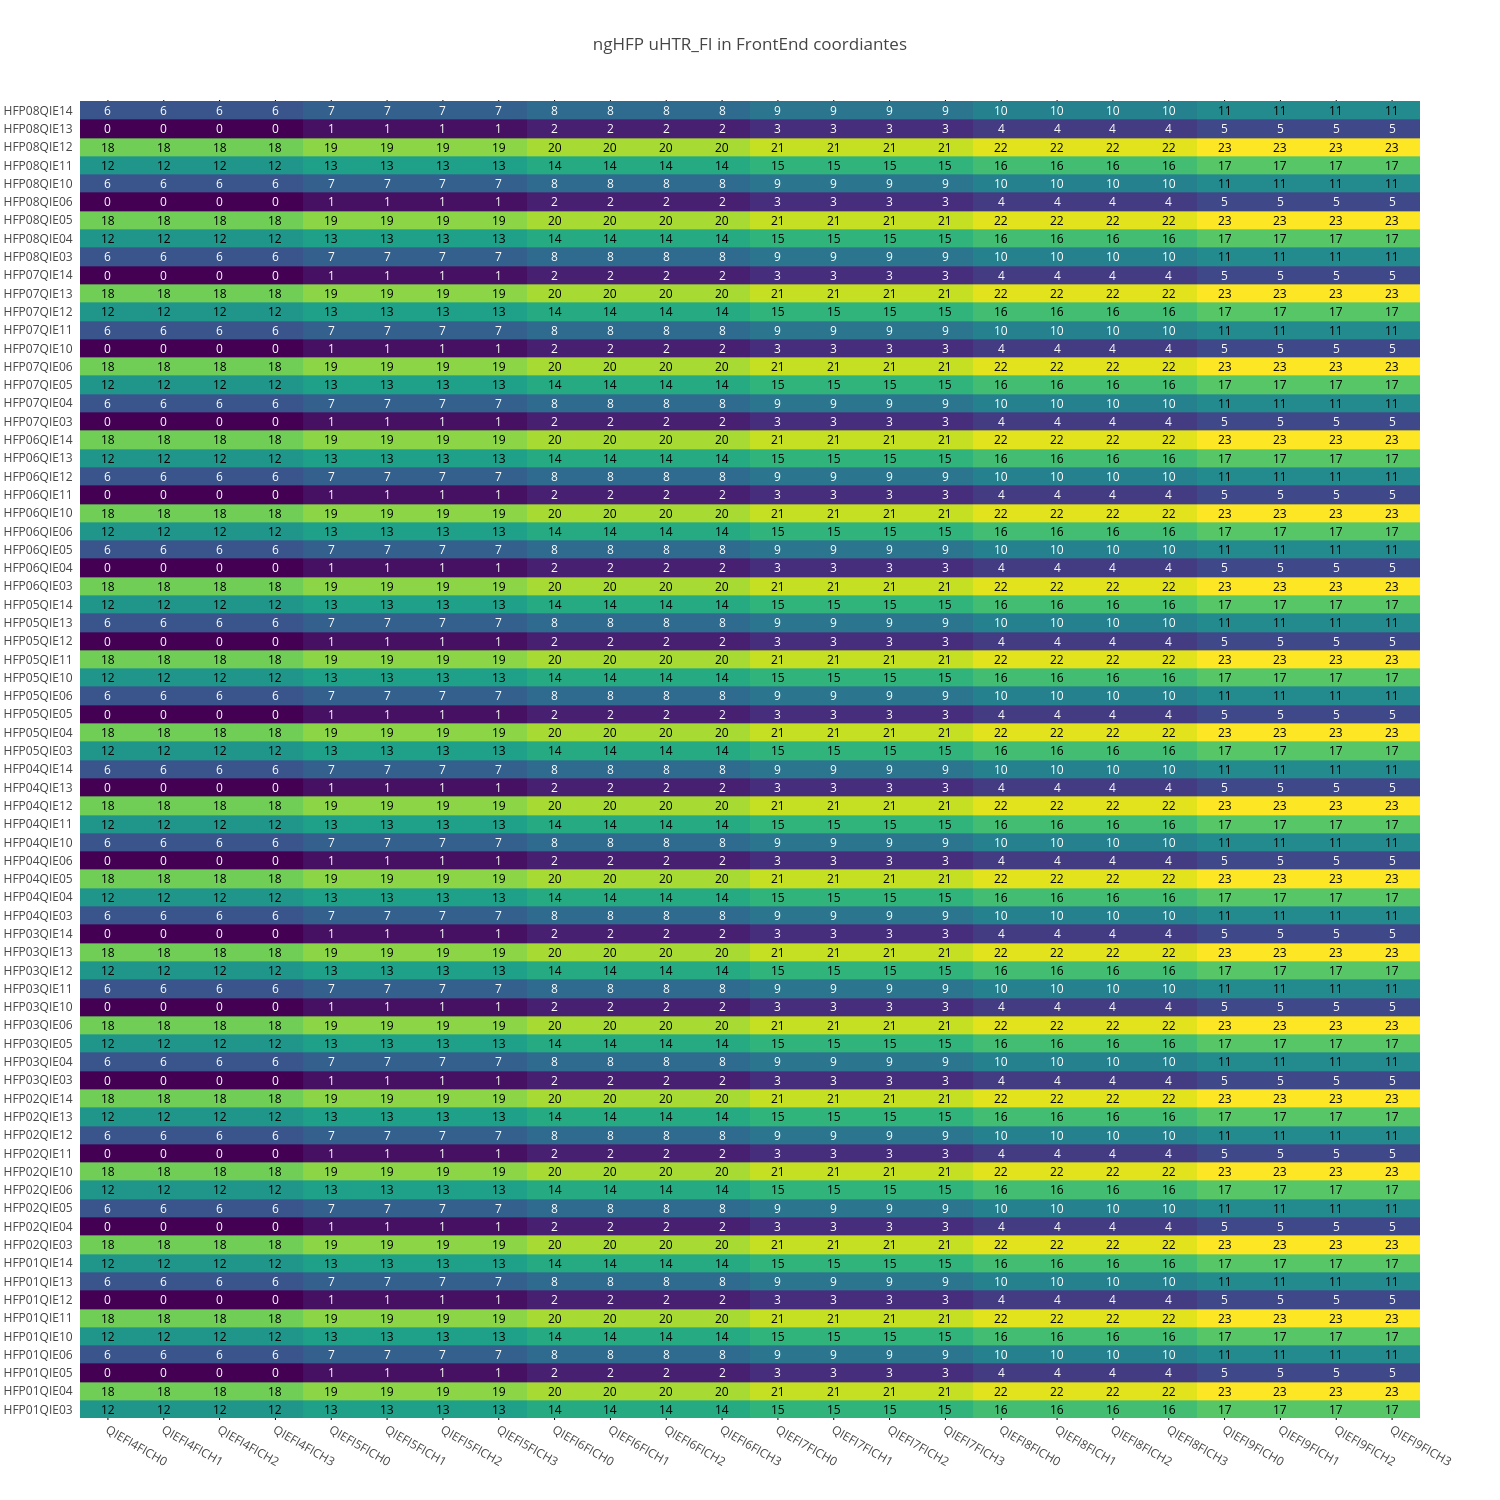
\includegraphics[angle=0,width=0.95\textwidth]{figures/appendix/ngHFP_uHTR_FI_in_FrontEnd.png}
  \end{tabular}
  \caption{HCAL (phase 1 HF, plus side) backend electronic coordinate uHTR fiber distribution in the frontend electronic coordinates.}
  \label{fig:lmapngHFPuHTRFIFEC}
 \end{center}
\end{figure}
\clearpage

\begin{figure}[htb]
 \begin{center}
  \begin{tabular}{cc}
   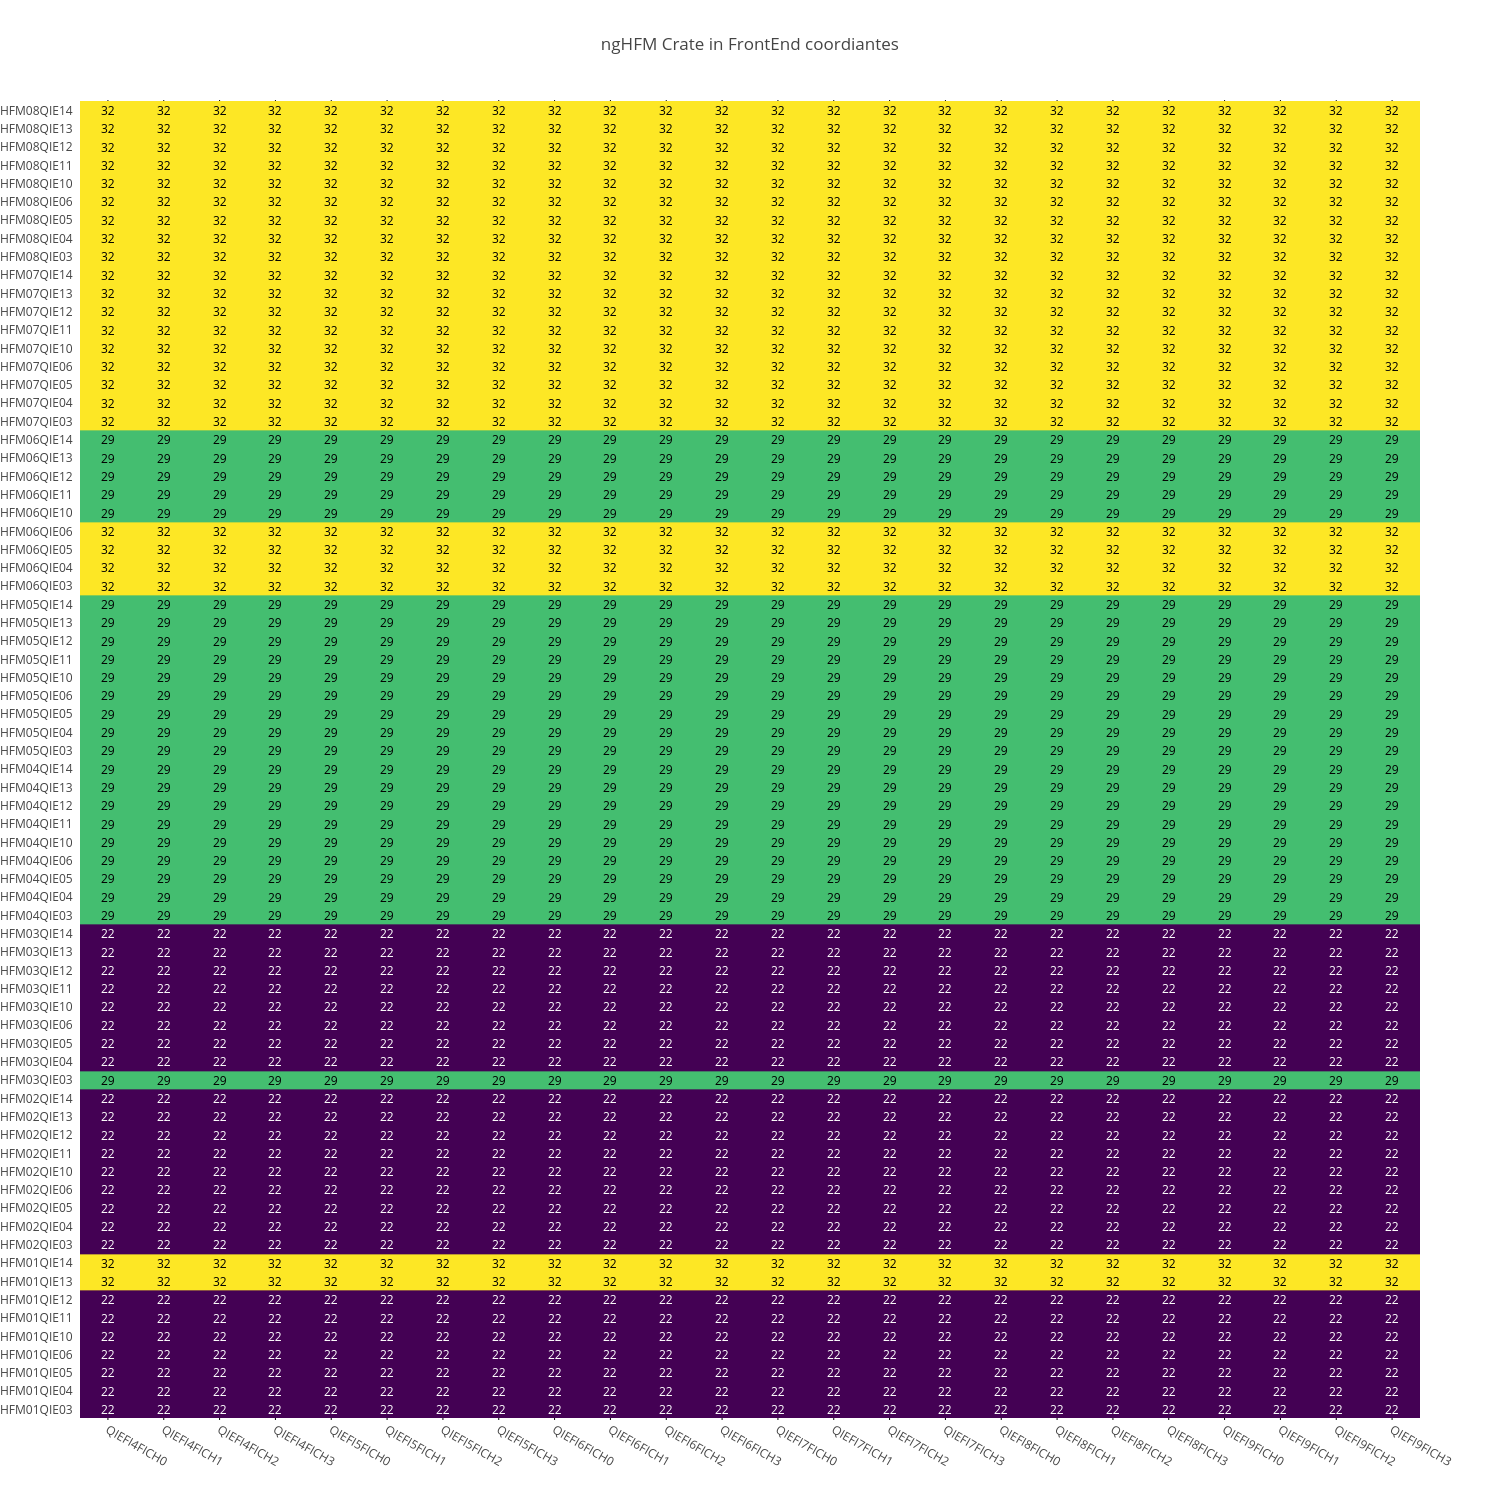
\includegraphics[angle=0,width=0.95\textwidth]{figures/appendix/ngHFM_Crate_in_FrontEnd.png}
  \end{tabular}
  \caption{HCAL (phase 1 HF, minus side) backend electronic coordinate crate distribution in the frontend electronic coordinates.}
  \label{fig:lmapngHFMCrateFEC}
 \end{center}
\end{figure}
\clearpage

\begin{figure}[htb]
 \begin{center}
  \begin{tabular}{cc}
   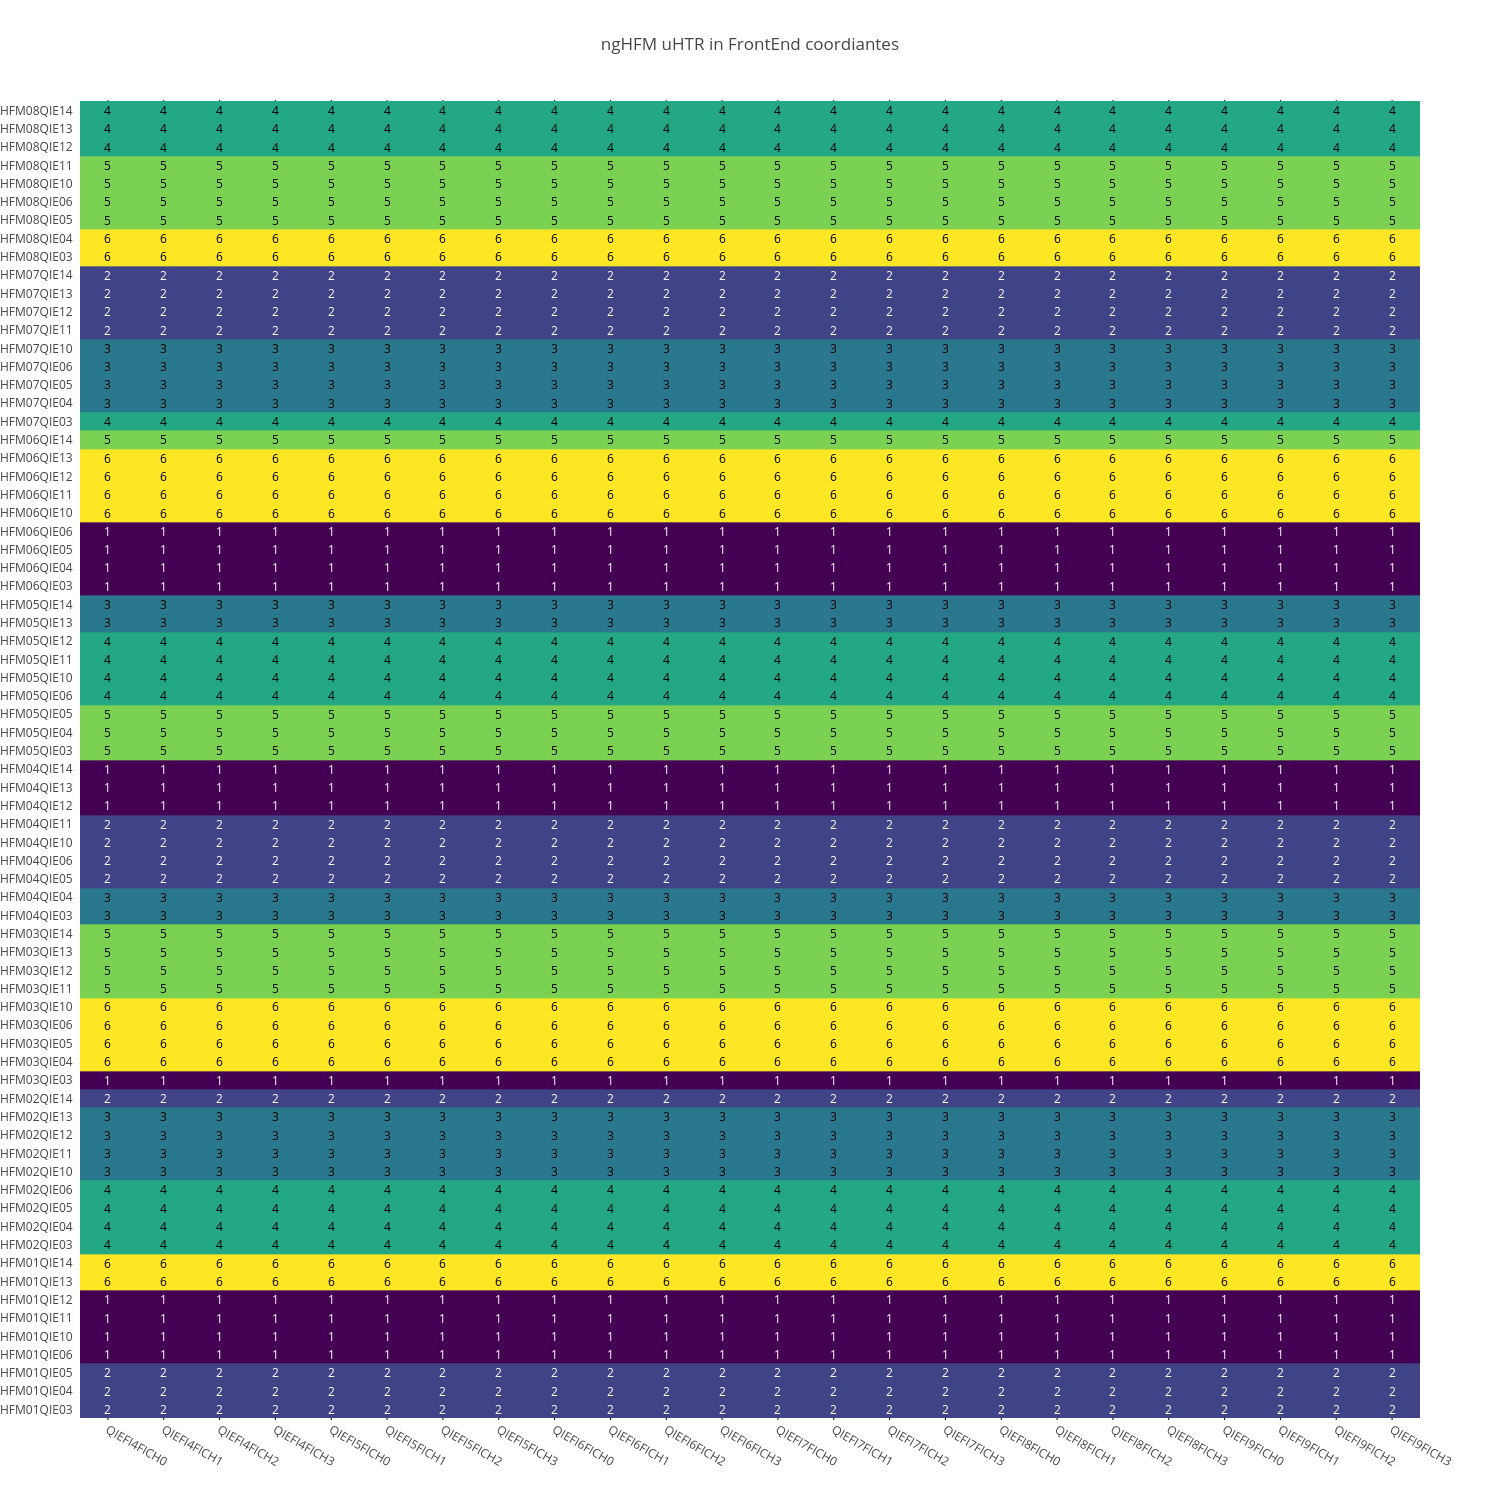
\includegraphics[angle=0,width=0.95\textwidth]{figures/appendix/ngHFM_uHTR_in_FrontEnd.png}
  \end{tabular}
  \caption{HCAL (phase 1 HF, minus side) backend electronic coordinate uHTR slot distribution in the frontend electronic coordinates.}
  \label{fig:lmapngHFMuHTRFEC}
 \end{center}
\end{figure}
\clearpage

\begin{figure}[htb]
 \begin{center}
  \begin{tabular}{cc}
   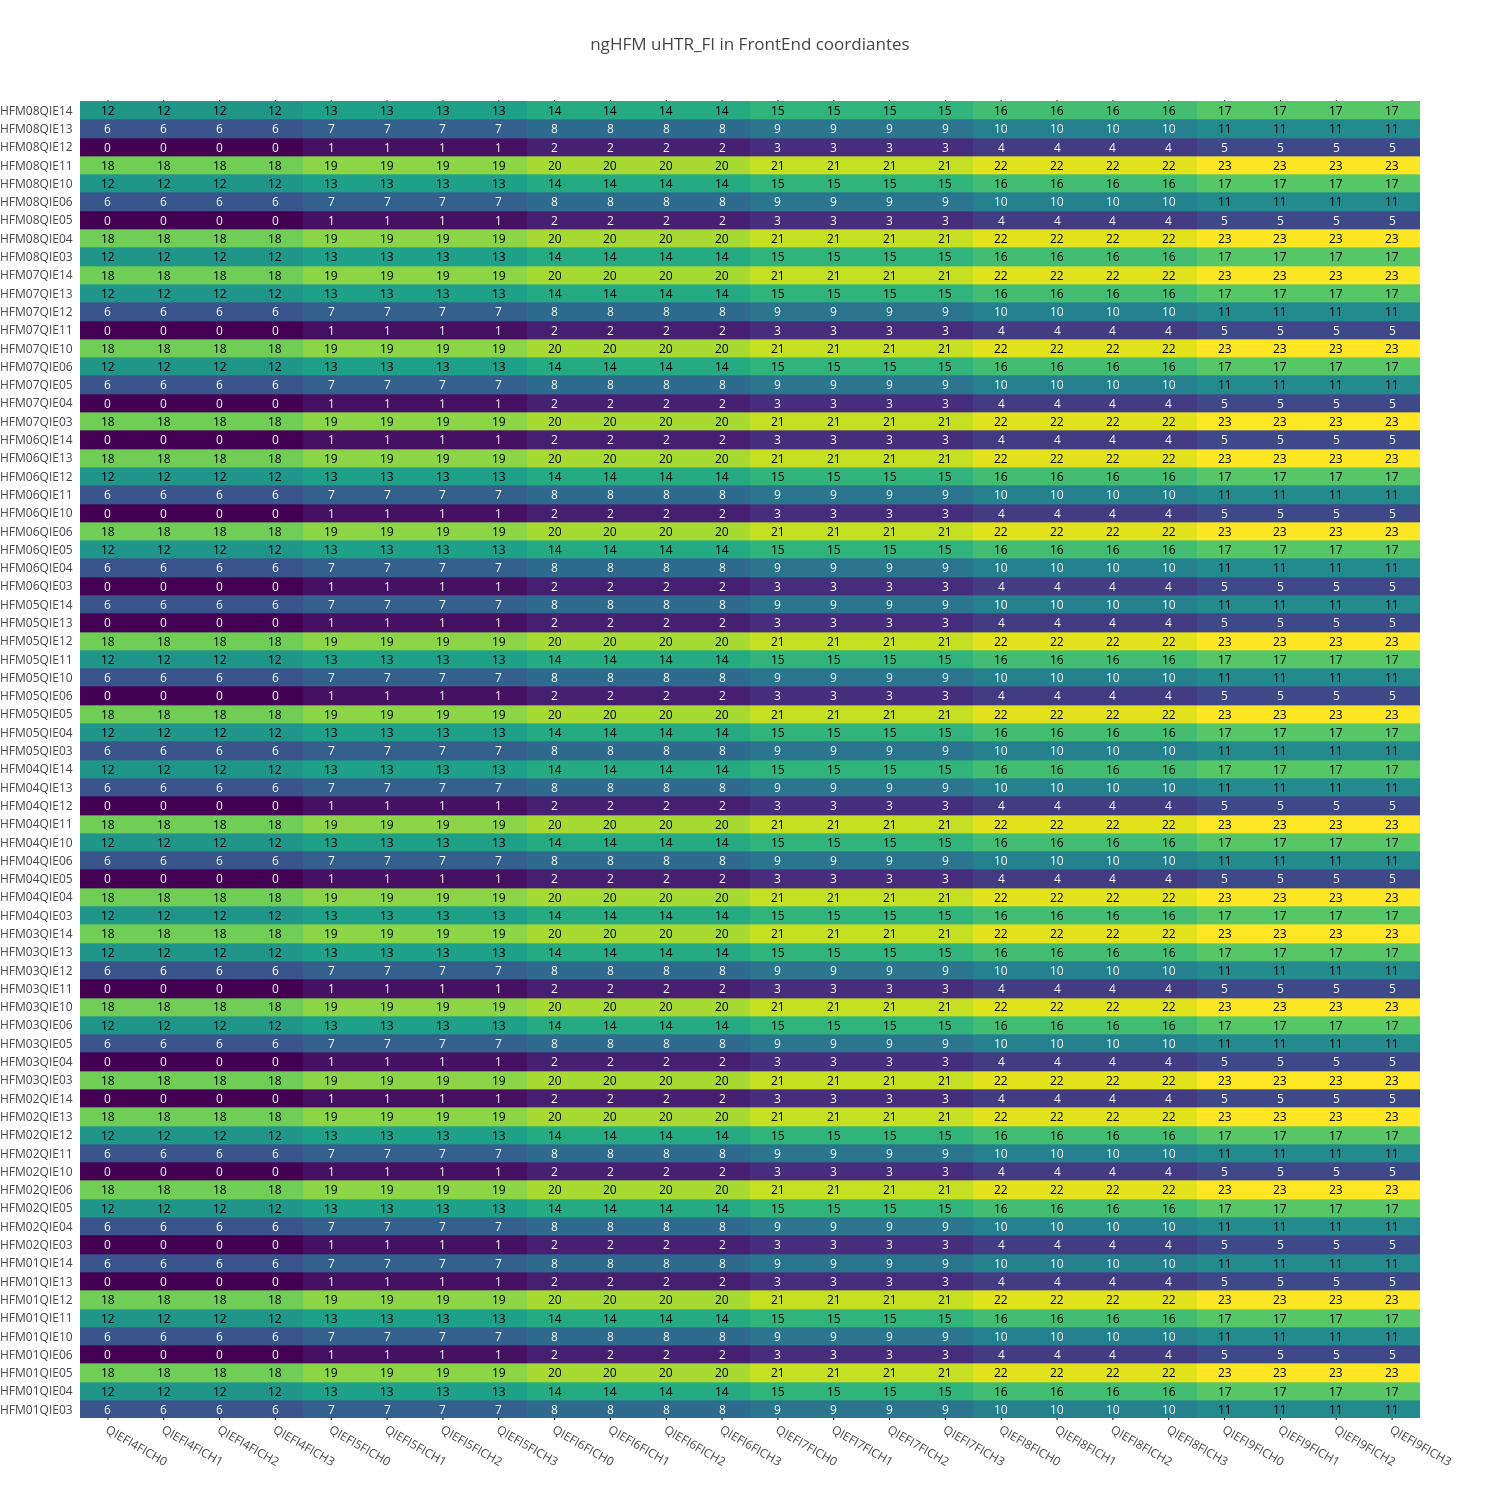
\includegraphics[angle=0,width=0.95\textwidth]{figures/appendix/ngHFM_uHTR_FI_in_FrontEnd.png}
  \end{tabular}
  \caption{HCAL (phase 1 HF, minus side) backend electronic coordinate uHTR fiber distribution in the frontend electronic coordinates.}
  \label{fig:lmapngHFMuHTRFIFEC}
 \end{center}
\end{figure}
\clearpage

\subsection{HO since 2015}
HO has been in SiPM+QIE8 FrontEnd+VME BackEnd stage since long shutdown 1. Unlike HB, HE and HF, HO geometry scheme is more similar to muon system. There are 5 wheels in HO, labeled from -2 to +2. The central wheel (wheel 0) has 12 readout boxes per wheel, 3 readout modules per box. The other wheels have 6 readout boxes per wheel, 4 readout modules per box. HO patch panels are organized in 2015 on requirements of the trigger bits delivered to muon system (TwinMUX). 

The HO validation plots are shown from Fig~\ref{fig:lmapHO0EtaFEC} to Fig~\ref{fig:lmapHO2MHTRFIFEC}. There are 2376 readout channels in HO. 2160 channels are physical readout channel. 216 channels are calibration channels, labeled as ``HOX". 144 of them are normal calibration channels, which connected to the patch panel and BackEnd electronics. The rest 72 HOX channels are even not connected to the patch panel. HO is the only HCAL sub-system that still use VME based BackEnd electronics. There are 4 VME crates for HO, 12 HTR per crate. Each HTR card has two FPGA, labeled as ``Top" or ``Bottom". There are 8 fibers comes out from each HTR card. Each fiber has 3 channels.
\clearpage

\begin{figure}[htb]
 \begin{center}
  \begin{tabular}{cc}
   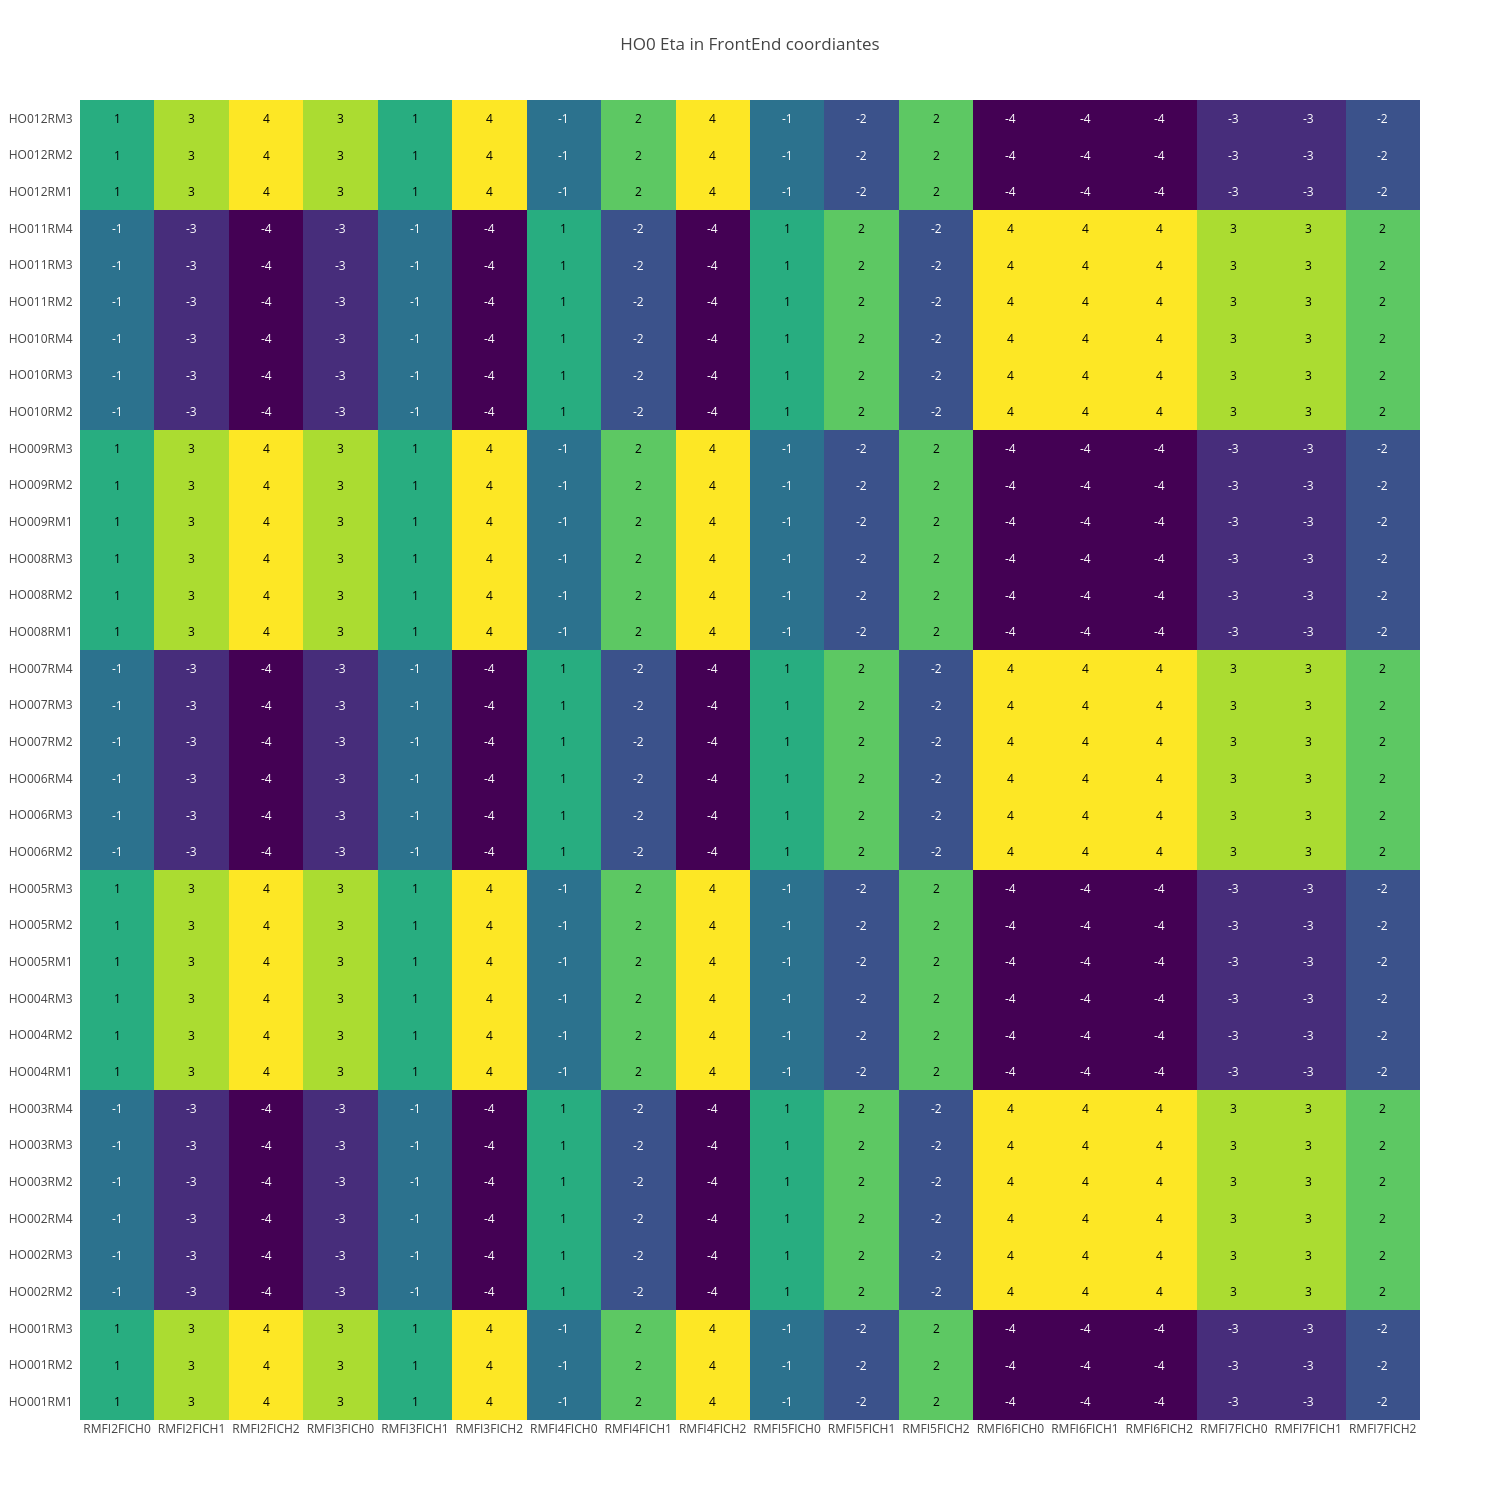
\includegraphics[angle=0,width=0.95\textwidth]{figures/appendix/HO0_Eta_in_FrontEnd.png}
  \end{tabular}
	\caption{HCAL (phase 1 HO, sector 0) detector $\eta$ distribution in the frontend electronic coordinates.}
  \label{fig:lmapHO0EtaFEC}
 \end{center}
\end{figure}
\clearpage

\begin{figure}[htb]
 \begin{center}
  \begin{tabular}{cc}
   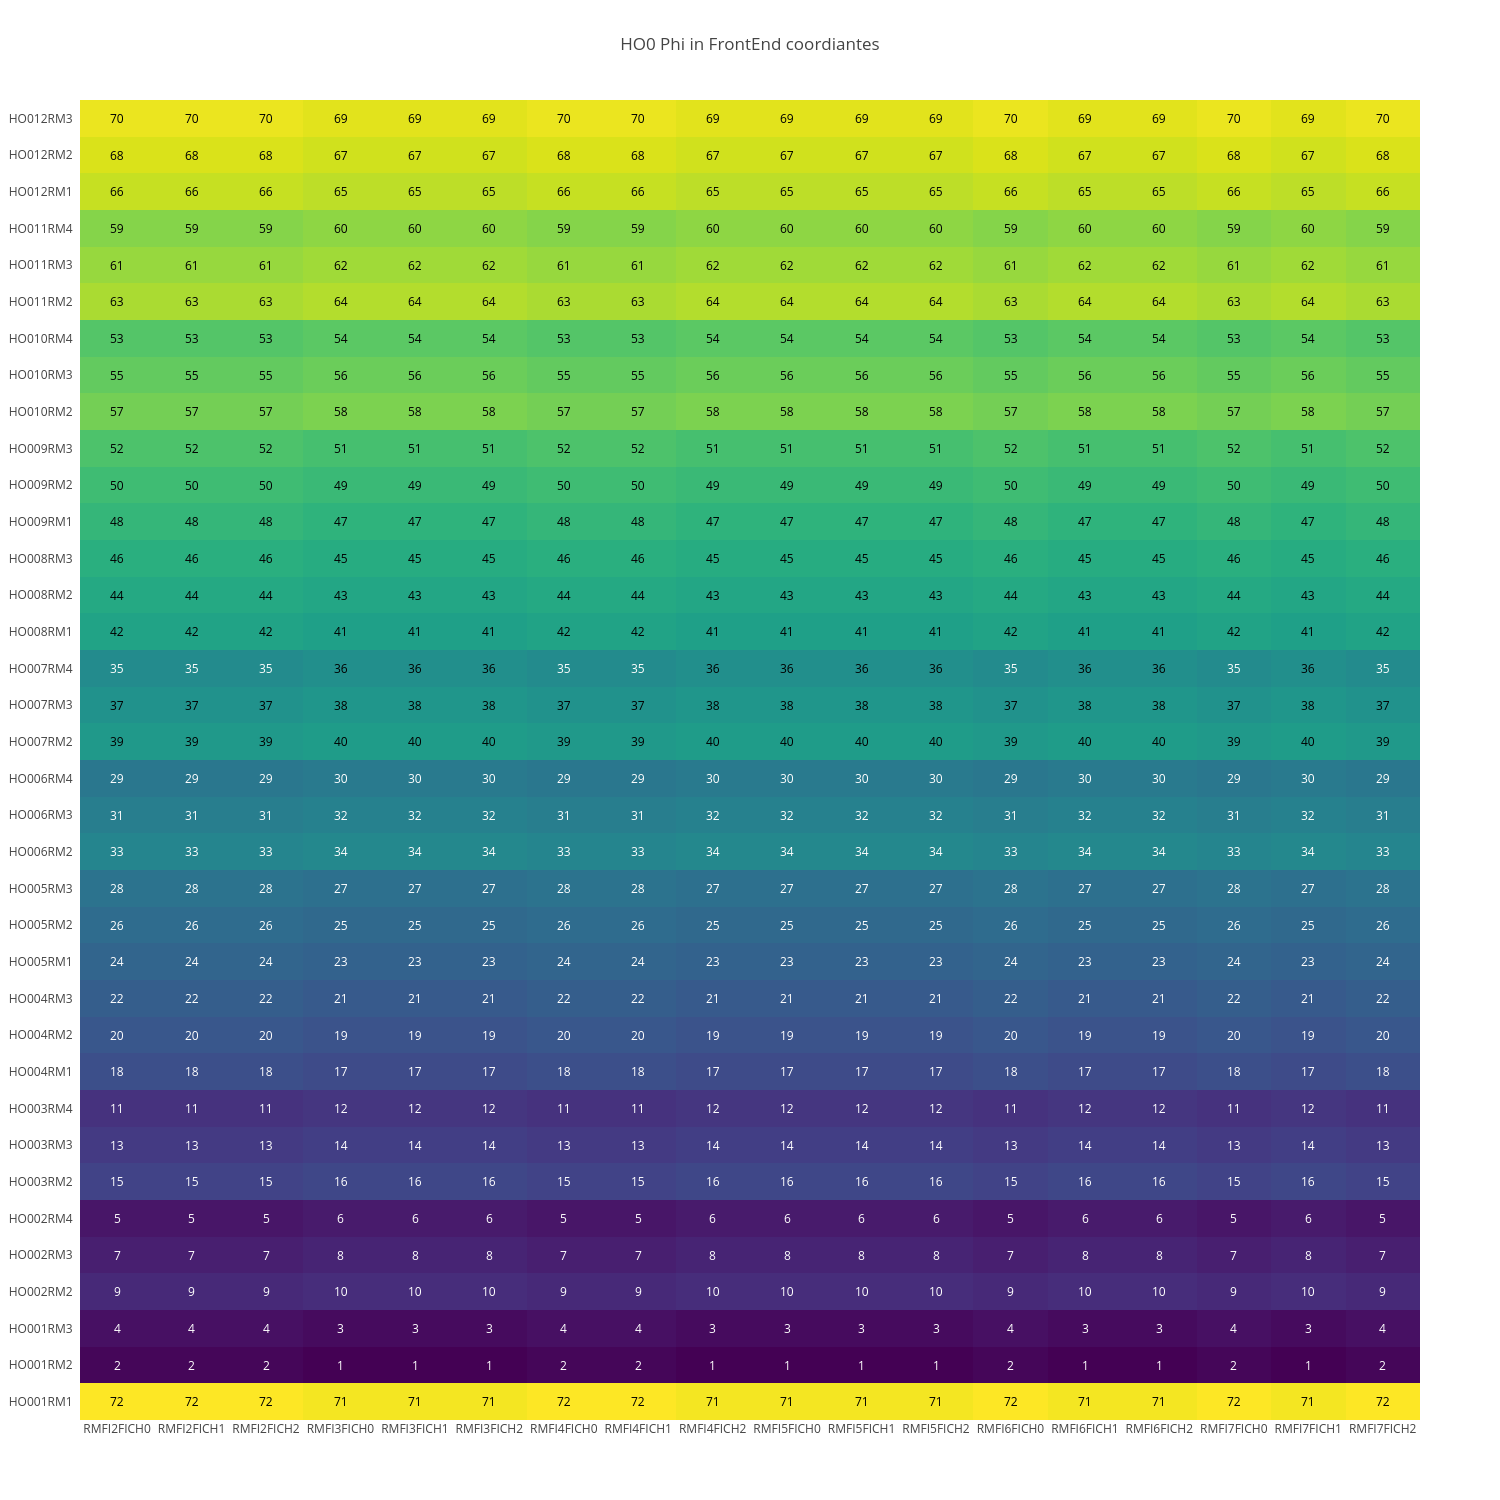
\includegraphics[angle=0,width=0.95\textwidth]{figures/appendix/HO0_Phi_in_FrontEnd.png}
  \end{tabular}
	\caption{HCAL (phase 1 HO, sector 0) detector $\phi$ distribution in the frontend electronic coordinates.}
  \label{fig:lmapHO0PhiFEC}
 \end{center}
\end{figure}
\clearpage

\begin{figure}[htb]
 \begin{center}
  \begin{tabular}{cc}
   \includegraphics[angle=0,width=0.95\textwidth]{figures/appendix/HO1P_Eta_in_FrontEnd.png}
  \end{tabular}
  \caption{HCAL (phase 1 HO, sector 1, plus side) detector $\eta$ distribution in the frontend electronic coordinates.}
  \label{fig:lmapHO1PEtaFEC}
 \end{center}
\end{figure}
\clearpage

\begin{figure}[htb]
 \begin{center}
  \begin{tabular}{cc}
   \includegraphics[angle=0,width=0.95\textwidth]{figures/appendix/HO1P_Phi_in_FrontEnd.png}
  \end{tabular}
  \caption{HCAL (phase 1 HO, sector 1, plus side) detector $\phi$ distribution in the frontend electronic coordinates.}
  \label{fig:lmapHO1PPhiFEC}
 \end{center}
\end{figure}
\clearpage

\begin{figure}[htb]
 \begin{center}
  \begin{tabular}{cc}
   \includegraphics[angle=0,width=0.95\textwidth]{figures/appendix/HO1M_Eta_in_FrontEnd.png}
  \end{tabular}
  \caption{HCAL (phase 1 HO, sector 1, minus side) detector $\eta$ distribution in the frontend electronic coordinates.}
  \label{fig:lmapHO1MEtaFEC}
 \end{center}
\end{figure}
\clearpage

\begin{figure}[htb]
 \begin{center}
  \begin{tabular}{cc}
   \includegraphics[angle=0,width=0.95\textwidth]{figures/appendix/HO1M_Phi_in_FrontEnd.png}
  \end{tabular}
  \caption{HCAL (phase 1 HO, sector 1, minus side) detector $\phi$ distribution in the frontend electronic coordinates.}
  \label{fig:lmapHO1MPhiFEC}
 \end{center}
\end{figure}
\clearpage

\begin{figure}[htb]
 \begin{center}
  \begin{tabular}{cc}
   \includegraphics[angle=0,width=0.95\textwidth]{figures/appendix/HO2P_Eta_in_FrontEnd.png}
  \end{tabular}
  \caption{HCAL (phase 1 HO, sector 2, plus side) detector $\eta$ distribution in the frontend electronic coordinates.}
  \label{fig:lmapHO2PEtaFEC}
 \end{center}
\end{figure}
\clearpage

\begin{figure}[htb]
 \begin{center}
  \begin{tabular}{cc}
   \includegraphics[angle=0,width=0.95\textwidth]{figures/appendix/HO2P_Phi_in_FrontEnd.png}
  \end{tabular}
  \caption{HCAL (phase 1 HO, sector 2, plus side) detector $\phi$ distribution in the frontend electronic coordinates.}
  \label{fig:lmapHO2PPhiFEC}
 \end{center}
\end{figure}
\clearpage

\begin{figure}[htb]
 \begin{center}
  \begin{tabular}{cc}
   \includegraphics[angle=0,width=0.95\textwidth]{figures/appendix/HO2M_Eta_in_FrontEnd.png}
  \end{tabular}
  \caption{HCAL (phase 1 HO, sector 2, minus side) detector $\eta$ distribution in the frontend electronic coordinates.}
  \label{fig:lmapHO2MEtaFEC}
 \end{center}
\end{figure}
\clearpage

\begin{figure}[htb]
 \begin{center}
  \begin{tabular}{cc}
   \includegraphics[angle=0,width=0.95\textwidth]{figures/appendix/HO1M_Phi_in_FrontEnd.png}
  \end{tabular}
  \caption{HCAL (phase 1 HO, sector 2, minus side) detector $\phi$ distribution in the frontend electronic coordinates.}
  \label{fig:lmapHO2MPhiFEC}
 \end{center}
\end{figure}
\clearpage

\begin{figure}[htb]
 \begin{center}
  \begin{tabular}{cc}
   \includegraphics[angle=0,width=0.95\textwidth]{figures/appendix/HO0_Crate_in_FrontEnd.png}
  \end{tabular}
  \caption{HCAL (phase 1 HO, sector 0) backend electronic coordinate crate distribution in the frontend electronic coordinates.}
  \label{fig:lmapHO0CrateFEC}
 \end{center}
\end{figure}
\clearpage

\begin{figure}[htb]
 \begin{center}
  \begin{tabular}{cc}
   \includegraphics[angle=0,width=0.95\textwidth]{figures/appendix/HO0_HTR_in_FrontEnd.png}
  \end{tabular}
  \caption{HCAL (phase 1 HO, sector 0) backend electronic coordinate HTR slot distribution in the frontend electronic coordinates.}
  \label{fig:lmapHO0HTRFEC}
 \end{center}
\end{figure}
\clearpage

\begin{figure}[htb]
 \begin{center}
  \begin{tabular}{cc}
   \includegraphics[angle=0,width=0.95\textwidth]{figures/appendix/HO0_HTR_TB_in_FrontEnd.png}
  \end{tabular}
  \caption{HCAL (phase 1 HO, sector 0) backend electronic coordinate HTR fpga distribution in the frontend electronic coordinates.}
  \label{fig:lmapHO0HTRTBFEC}
 \end{center}
\end{figure}
\clearpage

\begin{figure}[htb]
 \begin{center}
  \begin{tabular}{cc}
   \includegraphics[angle=0,width=0.95\textwidth]{figures/appendix/HO0_HTR_FI_in_FrontEnd.png}
  \end{tabular}
  \caption{HCAL (phase 1 HO, sector 0) backend electronic coordinate HTR fiber distribution in the frontend electronic coordinates.}
  \label{fig:lmapHO0HTRFIFEC}
 \end{center}
\end{figure}
\clearpage

\begin{figure}[htb]
 \begin{center}
  \begin{tabular}{cc}
   \includegraphics[angle=0,width=0.95\textwidth]{figures/appendix/HO1P_Crate_in_FrontEnd.png}
  \end{tabular}
  \caption{HCAL (phase 1 HO, sector 1, plus side) backend electronic coordinate crate distribution in the frontend electronic coordinates.}
  \label{fig:lmapHO1PCrateFEC}
 \end{center}
\end{figure}
\clearpage

\begin{figure}[htb]
 \begin{center}
  \begin{tabular}{cc}
   \includegraphics[angle=0,width=0.95\textwidth]{figures/appendix/HO1P_HTR_in_FrontEnd.png}
  \end{tabular}
  \caption{HCAL (phase 1 HO, sector 1, plus side) backend electronic coordinate HTR slot distribution in the frontend electronic coordinates.}
  \label{fig:lmapHO1PHTRFEC}
 \end{center}
\end{figure}
\clearpage

\begin{figure}[htb]
 \begin{center}
  \begin{tabular}{cc}
   \includegraphics[angle=0,width=0.95\textwidth]{figures/appendix/HO1P_HTR_TB_in_FrontEnd.png}
  \end{tabular}
  \caption{HCAL (phase 1 HO, sector 1, plus side) backend electronic coordinate HTR fpga distribution in the frontend electronic coordinates.}
  \label{fig:lmapHO1PHTRTBFEC}
 \end{center}
\end{figure}
\clearpage

\begin{figure}[htb]
 \begin{center}
  \begin{tabular}{cc}
   \includegraphics[angle=0,width=0.95\textwidth]{figures/appendix/HO1P_HTR_FI_in_FrontEnd.png}
  \end{tabular}
  \caption{HCAL (phase 1 HO, sector 1, plus side) backend electronic coordinate HTR fiber distribution in the frontend electronic coordinates.}
  \label{fig:lmapHO1PHTRFIFEC}
 \end{center}
\end{figure}
\clearpage

\begin{figure}[htb]
 \begin{center}
  \begin{tabular}{cc}
   \includegraphics[angle=0,width=0.95\textwidth]{figures/appendix/HO1M_Crate_in_FrontEnd.png}
  \end{tabular}
  \caption{HCAL (phase 1 HO, sector 1, minus side) backend electronic coordinate crate distribution in the frontend electronic coordinates.}
  \label{fig:lmapHO1MCrateFEC}
 \end{center}
\end{figure}
\clearpage

\begin{figure}[htb]
 \begin{center}
  \begin{tabular}{cc}
   \includegraphics[angle=0,width=0.95\textwidth]{figures/appendix/HO1M_HTR_in_FrontEnd.png}
  \end{tabular}
  \caption{HCAL (phase 1 HO, sector 1, minus side) backend electronic coordinate HTR slot distribution in the frontend electronic coordinates.}
  \label{fig:lmapHO1MHTRFEC}
 \end{center}
\end{figure}
\clearpage

\begin{figure}[htb]
 \begin{center}
  \begin{tabular}{cc}
   \includegraphics[angle=0,width=0.95\textwidth]{figures/appendix/HO1M_HTR_TB_in_FrontEnd.png}
  \end{tabular}
  \caption{HCAL (phase 1 HO, sector 1, minus side) backend electronic coordinate HTR fpga distribution in the frontend electronic coordinates.}
  \label{fig:lmapHO1MHTRTBFEC}
 \end{center}
\end{figure}
\clearpage

\begin{figure}[htb]
 \begin{center}
  \begin{tabular}{cc}
   \includegraphics[angle=0,width=0.95\textwidth]{figures/appendix/HO1M_HTR_FI_in_FrontEnd.png}
  \end{tabular}
  \caption{HCAL (phase 1 HO, sector 1, minus side) backend electronic coordinate HTR fiber distribution in the frontend electronic coordinates.}
  \label{fig:lmapHO1MHTRFIFEC}
 \end{center}
\end{figure}
\clearpage

\begin{figure}[htb]
 \begin{center}
  \begin{tabular}{cc}
   \includegraphics[angle=0,width=0.95\textwidth]{figures/appendix/HO2P_Crate_in_FrontEnd.png}
  \end{tabular}
  \caption{HCAL (phase 1 HO, sector 2, plus side) backend electronic coordinate crate distribution in the frontend electronic coordinates.}
  \label{fig:lmapHO2PCrateFEC}
 \end{center}
\end{figure}
\clearpage

\begin{figure}[htb]
 \begin{center}
  \begin{tabular}{cc}
   \includegraphics[angle=0,width=0.95\textwidth]{figures/appendix/HO2P_HTR_in_FrontEnd.png}
  \end{tabular}
  \caption{HCAL (phase 1 HO, sector 2, plus side) backend electronic coordinate HTR slot distribution in the frontend electronic coordinates.}
  \label{fig:lmapHO2PHTRFEC}
 \end{center}
\end{figure}
\clearpage

\begin{figure}[htb]
 \begin{center}
  \begin{tabular}{cc}
   \includegraphics[angle=0,width=0.95\textwidth]{figures/appendix/HO2P_HTR_TB_in_FrontEnd.png}
  \end{tabular}
  \caption{HCAL (phase 1 HO, sector 2, plus side) backend electronic coordinate HTR fpga distribution in the frontend electronic coordinates.}
  \label{fig:lmapHO2PHTRTBFEC}
 \end{center}
\end{figure}
\clearpage

\begin{figure}[htb]
 \begin{center}
  \begin{tabular}{cc}
   \includegraphics[angle=0,width=0.95\textwidth]{figures/appendix/HO2P_HTR_FI_in_FrontEnd.png}
  \end{tabular}
  \caption{HCAL (phase 1 HO, sector 2, plus side) backend electronic coordinate HTR fiber distribution in the frontend electronic coordinates.}
  \label{fig:lmapHO2PHTRFIFEC}
 \end{center}
\end{figure}
\clearpage

\begin{figure}[htb]
 \begin{center}
  \begin{tabular}{cc}
   \includegraphics[angle=0,width=0.95\textwidth]{figures/appendix/HO2M_Crate_in_FrontEnd.png}
  \end{tabular}
  \caption{HCAL (phase 1 HO, sector 2, minus side) backend electronic coordinate crate distribution in the frontend electronic coordinates.}
  \label{fig:lmapHO2MCrateFEC}
 \end{center}
\end{figure}
\clearpage

\begin{figure}[htb]
 \begin{center}
  \begin{tabular}{cc}
   \includegraphics[angle=0,width=0.95\textwidth]{figures/appendix/HO2M_HTR_in_FrontEnd.png}
  \end{tabular}
  \caption{HCAL (phase 1 HO, sector 2, minus side) backend electronic coordinate HTR slot distribution in the frontend electronic coordinates.}
  \label{fig:lmapHO2MHTRFEC}
 \end{center}
\end{figure}
\clearpage

\begin{figure}[htb]
 \begin{center}
  \begin{tabular}{cc}
   \includegraphics[angle=0,width=0.95\textwidth]{figures/appendix/HO2M_HTR_TB_in_FrontEnd.png}
  \end{tabular}
  \caption{HCAL (phase 1 HO, sector 2, minus side) backend electronic coordinate HTR fpga distribution in the frontend electronic coordinates.}
  \label{fig:lmapHO2MHTRTBFEC}
 \end{center}
\end{figure}
\clearpage

\begin{figure}[htb]
 \begin{center}
  \begin{tabular}{cc}
   \includegraphics[angle=0,width=0.95\textwidth]{figures/appendix/HO2M_HTR_FI_in_FrontEnd.png}
  \end{tabular}
  \caption{HCAL (phase 1 HO, sector 2, minus side) backend electronic coordinate HTR fiber distribution in the frontend electronic coordinates.}
  \label{fig:lmapHO2MHTRFIFEC}
 \end{center}
\end{figure}
\clearpage

\section{HCAL operation}
